\documentclass[12pt]{article}
\usepackage[margin=1in]{geometry}
\usepackage{lmodern}
\usepackage{amsmath,amssymb,amsthm,mathtools}
\usepackage{booktabs,threeparttable,graphicx,setspace,enumitem,longtable,array,tabularx}
\usepackage{xcolor}
\usepackage{etoolbox,needspace}
\AtBeginEnvironment{tabular}{\footnotesize}
\usepackage[authoryear,round]{natbib}
\usepackage{xr-hyper}
\usepackage[colorlinks=true,linkcolor=blue!50!black,citecolor=blue!50!black,urlcolor=blue!50!black]{hyperref}
\usepackage{fancyhdr}
\onehalfspacing
\emergencystretch=2em
\pagestyle{fancy}\fancyhf{}
\fancyhead[L]{\small Niroula, Niroula and Khatiwada}
\fancyhead[R]{\small Observationally Equivalent Algorithms}
\fancyfoot[C]{\thepage}
\renewcommand{\headrulewidth}{0.3pt}
\setlength{\headheight}{14pt}

\newtheorem{theorem}{Theorem}[section]
\newtheorem{proposition}[theorem]{Proposition}
\newtheorem{lemma}[theorem]{Lemma}
\newtheorem{corollary}[theorem]{Corollary}
\theoremstyle{definition}
\newtheorem{definition}[theorem]{Definition}
\newtheorem{assumption}[theorem]{Assumption}
\theoremstyle{remark}
\newtheorem{remark}[theorem]{Remark}
\newcommand{\E}{\mathbb{E}}
\newcommand{\R}{\mathbb{R}}
\newcommand{\KL}{D_{\mathrm{KL}}}
\newcommand{\lab}[1]{}
\title{Observationally Equivalent Algorithms:\\ What Prices Reveal About Trader Populations,\\ and What Supervisors Need}
\author{Pratik Niroula\thanks{Department of Computer Information Science, Minnesota State University, Mankato, MN 56001, USA. \texttt{pratik.niroula@mnsu.edu}.}
\and Prashant Niroula\,\thanks{Faculty of Management, Tribhuvan University, Kirtipur, Nepal. \texttt{prashantniroula20@gmail.com}.}
\and Sujan Khatiwada\thanks{Department of Electrical, Computer and Robotics Engineering, Minnesota State University, Mankato, MN 56001, USA. \texttt{sujan.khatiwada@mnsu.edu}.}}
\date{Working paper, 21 November 2026}

\usepackage{array}
\makeatletter\g@addto@macro\UrlBreaks{\do\_}\makeatother
\graphicspath{{../paper1_core/}}
\externaldocument[][nocite]{paper1b_companion}
\begin{document}
\maketitle
\thispagestyle{empty}\pagestyle{empty}
\begingroup\singlespacing\small

\begin{abstract}
\noindent Algorithmic traders read prices and, by trading, move them. We ask what the public record reveals about the population of such traders, and what supervisors need beyond it. When traders respond to a common public signal, the population affects prices, order flows and dealer inventories only through its aggregate feedback response, also in an inventory equilibrium. Learning anything finer is expensive: in the worst case, telling apart $K$ trader types whose rules lie within $\Delta$ of one another takes on the order of $\Delta^{-(4K-2)}$ observations, an order attained for linear memory rules. Given the market's own persistence and a bound on memory, a uniform cut in feedback can be set from prices, and without class tags it is minimax over the assignments of labels that the record allows; a targeted restriction cannot be set from prices. Class tags restore targeting only if relabeling is costly; an audit trail that links accounts to owners, and cannot be gamed, does not need that. Without tags, more data can leave the supervisor less informed, because an algorithm that fears targeting crowds toward its neighbour. A calibration to Taiwan's tagged exchange flows illustrates the barrier; a registered test there did not establish that the tagged responses are feedback. Core steps are checked in Lean~4.
\end{abstract}

\noindent\textbf{Supplement and companion.} The online supplement states every result in full, with proofs and machine-check details. Results on cascades after a breach, insiders, and nonlinear or learning traders are in a companion note \citep{niroula2026c}; references of the form C1.1 are to it.

\noindent\textbf{Keywords:} algorithmic trading, feedback trading, aggregate response, identification, supervision, disclosure. \textbf{JEL:} C32, D83, G14, G18.

\noindent\textbf{Code and proofs.} Baseline: \url{https://github.com/Pratikn03/Fianince}. Sources, build scripts and validation logs: \nolinkurl{research_extension/paper1_publication_revision/} in that repository.

\endgroup
\newpage
\pagestyle{fancy}
\setcounter{page}{1}

\section{Introduction}\label{n:intro}

\paragraph{The economic question.} A supervisor may know how strongly a market reacts to past prices while knowing little about which traders generate that response. These are different objects of inference. If every group's feedback is scaled by the same factor, the aggregate response is sufficient to evaluate the intervention in our model. If a particular group is halted, its contribution matters. This paper quantifies that distinction and the information supplied by class-tagged reports.

\paragraph{The answer.} Under a common public signal and fixed causal rules, the population enters public market outcomes through its aggregate flow map. For linear rules this map is the feedback kernel. Equal kernels give equal public paths, insider profits and dealer inventories under the same shocks and strategies; the resulting equilibrium correspondence uses the same strategy spaces and public payoff maps. Individual feedback traders' payoffs need not agree. A counterfactual that changes their strategies requires a separate invariance or equilibrium argument.

The same holds in equilibrium. Section~\ref{n:sec_equilibrium} derives price impact and the persistence of pricing errors from competitive dealers who carry inventory risk. The equilibrium price follows the same closed loop with effective parameters and unchanged memory rates, and the population enters only through the merged measure (Theorems~\ref{n:thm_inventory} and~\ref{n:thm_eqreduced}). The cost results below therefore apply when impact is an equilibrium outcome rather than an assumption.

    Four results organize the analysis. First, closely spaced types are weakly identified. A moment-matched pair of $K$-type populations has aggregate-flow differences of order $\Delta^{2K-1}$, leading to a Gaussian information lower bound of order $\Delta^{-(4K-2)}$. The smooth-family result requires common initial information, predictable probes and a derivative-moment bound uniform over the experiments being compared. It is a worst-case lower bound; some smooth families are never identified. Second, aggregate feedback can suffice for a decision even when the underlying population is hard to estimate. Proposition~\ref{n:target} gives the intervention comparison, and Corollary~\ref{n:decisionloss} expresses its consequence as expected decision loss. Third, reports that separately measure class flows change the observation experiment. In the exponential-memory model, tagging all but one memory class removes the spacing penalty for recovering class weights. An additional tag can still improve precision. Fourth, disclosure must survive the traders' response. When restricted traders can route activity through accounts that carry another label, class tags lose their value as relabeling becomes cheap and the best targeted restriction is partial, while an audit trail that links accounts to owners keeps its value (Proposition~\ref{n:relabel}).

\paragraph{What is new, and what is not.} The identification rate $\Delta^{-(4K-2)}$ is the known minimax rate for mixtures with near-colliding components \citep{heinrich2018,wu2020}; we use it and do not claim it. That market-wide policies need only a reduced-form aggregate while targeted ones need structure is Marschak's maxim and the logic of sufficient statistics for policy \citep{marschak1953,chetty2009}; what we add is the price of the structure in a feedback market. Sufficiency survives when price impact is an equilibrium outcome, and dealers' anticipation over-weights slow memories in equilibrium prices (Theorem~\ref{n:thm_eqreduced}). Which linear questions about the population prices answer cheaply is characterized exactly (Theorem~\ref{n:questions}). And the disclosure game has a sharp answer: class tags are worth only what relabeling costs, the share that hides does not depend on that cost, and an audit trail that links accounts to owners keeps its value, because we assume that it cannot be gamed. Without tags, a uniform policy is minimax over the labellings the record allows, for every convex loss, and with partial tags the minimax policy is uniform within each tagged group (Theorems~\ref{n:minimax} and~\ref{n:minimaxtags}). Finally, without tags more data can mean less information: an algorithm that fears targeting, facing a fixed test, crowds toward its neighbour fast enough that the supervisor's information about it falls like $N^{-1}$ as its record grows (Theorem~\ref{n:paradox}).

\paragraph{What a record reveals.} What a record reveals about which of two populations is trading equals the forecast loss from confusing them (Theorem~\ref{n:dual}), and a matching recovery bound holds within separated shrinking clusters (Theorem~\ref{n:shape}). Composition is not needed to forecast the public signal itself (Supplement Theorems~\ref{n:irr} and~\ref{n:uniformlog}). These results concern the observed pricing-error signal, not traded returns with hidden fundamentals.

\paragraph{Plan.} Section~\ref{n:model} sets out the model. Section~\ref{n:suff_sec} proves sufficiency and identification, and Section~\ref{n:sec_equilibrium} carries them to an inventory equilibrium. Section~\ref{n:cost_sec} prices composition, Section~\ref{n:irr_sec} equates what a record reveals with forecast loss, and Section~\ref{n:sup} turns to supervision and disclosure. Section~\ref{n:concl} records the evidence and the limits. Calendar-year conversions are illustrative, not estimates of any venue's identification horizon.

\subsection{Related literature}\label{n:lit}

The motivation is consistent with evidence of difficult parameter estimation in heterogeneous-agent models \citep{lux2018} and weak predictive content of large-trader positions in ten agricultural futures markets \citep{sanders2009}. Those findings neither identify the mechanism here nor test its intervention counterfactuals. The empirical exercises are reported with their registered outcomes and limitations.

\paragraph{What is known.} Exponential memory is the oldest model of expectations: adaptive expectations \citep{cagan1956,nerlove1958}, geometric distributed lags \citep{koyck1954}, and \citet{muth1960}'s proof that exponentially weighted forecasts are optimal for a random walk observed with noise. The idea that an aggregate depends on a distribution of individual coefficients and not on the individuals is also old. \citet{granger1980} showed it for sums of autoregressions, \citet{forni1997} developed the general theory of aggregation and dynamics, \citet{zaffaroni2004} and \citet{pesaran2014} the large-economy and large-panel versions, and recovering the distribution is the disaggregation problem \citep{celov2008}. Results of the form ``two structures give the same data, so data cannot choose'' have a famous precedent in \citet{sargent1976}, whose observational equivalence of natural and unnatural rate theories settled what reduced-form data could say about monetary rules. A large literature models markets with heterogeneous fundamentalist and chartist traders \citep{brock1998,hommes2006} and estimates their shares from prices \citep{boswijk2007,franke2012,lux2018}; our results say which features of a population such estimates can recover from prices, and at what cost, when demand is linear in past prices. \citet{auclert2024} make the corresponding sufficient-statistic argument for household heterogeneity in macroeconomics. That a decision needs only a reduction of the data is the subject of sufficiency and the comparison of experiments \citep{blackwell1953,lecam1964}, and control theory distinguishes identifying a system from having data that are informative enough for a control objective \citep{vanwaarde2020}. The rate $(\Delta\eta)^{-(4K-2)}$ is the known minimax rate for mixtures with near-colliding components \citep{heinrich2018,wu2020}, and the uniqueness step behind the stress result is the uniqueness of networks with one hidden layer \citep{sussmann1992}. The exponent $2K-1$ in the gap between near-colliding populations is also the error amplification for super-resolution of $K$ near-colliding point sources \citep{batenkov2021}, of which Prony's method is the classical instance. That disaggregate information helps forecast an aggregate when the components have different dynamics is known from the literature on forecasting aggregates \citep{lutkepohl1987,hendry2011}; the full working paper \citep{niroula2026full} states that result in this market. Feedback traders are central to models of destabilizing speculation and of return autocorrelation \citep{delong1990,cutler1990,sentana1992}; inventory-based price impact goes back to \citet{ho1981} and \citet{grossman1988}, and \citet{hendershott2014} measure it. Simulation-based estimation of agent-based models \citep{grazzini2015,platt2020} faces the same identification question in nonlinear models. Crowding among algorithmic and quantitative strategies is documented by \citet{chaboud2014} and \citet{khandani2011} and analysed by \citet{stein2009}, and anonymity in limit-order markets, which concerns who quotes rather than who trades on feedback, by \citet{foucault2007}. We do not claim these.

\paragraph{Trader identity in market microstructure.} Identity disclosure already has an established information role. \citet{linnainmaa2012} study investor information inferred from broker identity and order flow. \citet{frino2010} study how the information content of broker identity changes when trading becomes anonymous. Those mechanisms differ from the common-public-signal benchmark here, and show why a general irrelevance claim would be inappropriate. Our intervention comparison concerns estimating response coefficients and assigning restrictions, rather than establishing that identity can have value for price discovery.

\paragraph{Regulating algorithmic trading.} The policy debate turns on what supervisors can see. \citet{budish2015} trace the high-frequency arms race to the design of continuous limit order books and propose frequent batch auctions, a market-wide remedy. \citet{kirilenko2017} reconstruct the Flash Crash from account-level audit-trail data, classifying traders by their observed behaviour, and \citet{menkveld2016} surveys the economics of high-frequency trading. In the United States, SEC Rule~613 created the Consolidated Audit Trail, which links orders to customers across venues \citep{sec2012cat}. Our results give one reason for that architecture: a market-wide remedy can be calibrated from prices, a class restriction needs class records, and when traders can relabel, those records must be tied to owners (Proposition~\ref{n:relabel}).

\paragraph{Contribution relative to existing methods.} The statistical exponent and moment-matching method have close antecedents in finite-mixture estimation and super-resolution. Our contribution is their use in an endogenous feedback market with explicit observation contracts, combined with a comparison of common and class-specific interventions. Sufficiency is pathwise under common causal strategies; the price response identifies memory rates as transmission zeros, both under mechanical impact and in the inventory equilibrium of Section~\ref{n:sec_equilibrium}. Partial disclosure changes the number of untagged classes, pooling uses shared rates with diverse market weights, and hard limits separate calm-path equivalence from stress identification. These are conditional market results. Local numerical rank checks do not establish global identification, and a lower bound alone does not provide an attainable rate for every smooth family.

\section{Model}\label{n:model}

Time is discrete. Let $x_t$ be the pricing error, the gap between the price and the fundamental value. A reduced-form dealer sector absorbs net order flow with price impact $\kappa>0$, and arbitrage pulls the error toward zero with persistence $a\in[0,1)$. There are $K$ groups of feedback traders, with $0<\eta_i<1$ unless a boundary case is explicitly stated. Group $i$ keeps an exponentially weighted average $y_{i,t}$ of past pricing errors and trades $q_iy_{i,t}$:
\begin{equation}\label{n:eq:model}
x_t=ax_{t-1}+\kappa\sum_{i=1}^Kq_iy_{i,t-1}+\kappa v_t+\varepsilon_t,\qquad y_{i,t}=(1-\eta_i)y_{i,t-1}+\eta_ix_t,
\end{equation}
where $v_t$ is a probe, a trade by an observer, and $\varepsilon_t$ is news. A desk that tracks a trend with a steady-state Kalman filter \citep{muth1960}, or that learns by regularized online gradient descent, updates exactly this way (Supplement Lemma~\ref{lem:micro}). Write $r_i=1-\eta_i$ for the memory rate and $w_i=q_i\eta_i$ for the trading weight. The \emph{merged measure} $M=\sum_iw_i\delta_{r_i}$ puts weight $w_i$ at rate $r_i$, merging groups with equal rates, and the \emph{feedback kernel} is its sequence of moments,
\[
k_m=\sum_iw_ir_i^{\,m},\qquad m=0,1,2,\ldots
\]
Total feedback flow is the convolution of past prices with $k$. The \emph{feedback budget} $S=a+\kappa\sum_iq_i=a+\kappa\sum_mk_m$ governs stability: with $q_i\ge0$ the market is stable exactly when $S<1$.

\paragraph{Observed signal.} In the reduced-form results the observer sees $x_t$, or a public signal from which it is reconstructible. If fundamental value is hidden, traded prices alone need not reveal pricing errors. Section~\ref{n:irr_sec} separates these observation regimes. The dynamic sufficiency theorem uses a signal explicitly measurable from public history.

\paragraph{The observer.} The cost results concern a supervisor or exchange that knows $(a,\kappa)$ and the noise law. It can wait and record prices, probe from a reset state and record the response, probe the running market with random signs (which costs the same order of data, \citealp[Theorem~S16.1]{niroula2026full}), or receive class-tagged flow reports. Reset probing is a benchmark for what data can reveal, not a proposed policy. Knowing $(a,\kappa)$ only helps the observer, so the lower bounds below hold a fortiori when $(a,\kappa)$ must be estimated.

\paragraph{When impact is mechanical.} Model \eqref{n:eq:model} lets feedback flow move the price. That describes markets in which prices are set by the mechanics of a limit order book or an automated market maker, or by dealers who price flow by its effect on their inventory (Supplement Theorem~\ref{thm:inventory}). It does not describe a market maker who sets prices as conditional expectations of value and knows the aggregate flow rule. Feedback flow is then predictable from past prices, is netted out and moves no price, so prices are those of a market without feedback traders and reveal nothing about them (Companion Proposition~\ref{prop:insider}(iv)). Sufficiency (Theorem~\ref{n:suff}) holds for any dealer rule. The identification and cost results are stated for mechanical impact; the barrier they describe is not an artefact of it, since with a fully rational market maker prices reveal less, not more.

\section{The kernel is sufficient and is what prices identify}\label{n:suff_sec}

For sufficiency we embed the groups in a general market. A value $v$ is drawn, noise traders submit $z_t$, an insider submits $X_t(v,\mathcal H_{t-1})$, and a dealer sets the price $P_t(\mathcal H_{t-1},y_t)$ from the public history and the total order flow $y_t$. The groups update on a public signal $s_t=S_t(p_0,\ldots,p_t)$ and contribute flow $f_t=\sum_{m<t}k_ms_{t-1-m}$. The maps $X$, $P$ and $S$ are arbitrary causal rules. The strategic players in the equivalence below are the insider and dealer; feedback-group rules are fixed and their individual payoffs are not part of the payoff equivalence.

\begin{theorem}[The kernel is sufficient]\label{n:suff}
If two group configurations have $k_m=k'_m$ for $m<T$, then for every strategy profile and every realization of $(v,z)$ the price and order-flow paths, the insider's trades and realized profit, and the dealer's inventory coincide on dates $t\le T$. The two games have the same strategy sets and payoffs, and hence the same equilibria under any concept defined from payoffs and the public history. The same holds for any finite population whose flows are causal linear functions of the public signal, with $k$ the sum of the individual kernels. Group-level quantities, such as the weight of the largest group, are not invariant.
\end{theorem}

The proof is an induction on dates (Supplement Theorem~\ref{thm:eqinv} and Proposition~\ref{prop:anylinear}). It is short; its content is the object it isolates, a population-level quantity that settles every equilibrium concept at once. The induction uses only that aggregate feedback flow is a fixed causal function of the public signal. So for any population, linear or not, including traders who switch strategies after observing past profits, the aggregate flow map is sufficient (machine-checked in this generality; \citealp[Theorem~S6.1]{niroula2026full}); the kernel is that map when flows are linear. Equal kernels remain observationally equivalent when anonymous aggregate flow is added to the public record. This does not imply that flow reports cannot improve finite-sample precision or reveal more than prices under another dealer rule. For example, a dealer that always quotes zero hides every kernel in prices, while a deterministic public signal equal to one makes the first aggregate feedback flow reveal $k_0$. The converse identification statement below needs the specified mechanical-impact experiment.

\begin{theorem}[What prices identify]\label{n:ident}
In model \eqref{n:eq:model}, fix common known $(a,\kappa)$ and zero initial group states, and compare noiseless probe responses. Two economies produce identical price responses to every probe sequence if and only if their merged measures coincide.
\end{theorem}

This is Supplement Theorem~\ref{thm:merged}(i). The same holds when $\kappa$ and $a$ are derived from competitive dealers who dislike inventory: the equilibrium price follows \eqref{n:eq:model} path by path with effective impact and persistence, and with the memory rates unchanged (Theorems~\ref{n:thm_inventory} and~\ref{n:thm_eqreduced}).

Together, Theorems~\ref{n:suff} and~\ref{n:ident} make the kernel a \emph{minimal identifying functional} of the population for prices: it determines everything prices can show, and prices determine it. (The merged measure has finitely many atoms, so its moments, the kernel, determine it.)


\section{Sufficiency and identification in equilibrium}\label{n:sec_equilibrium}

The identification results of Section~\ref{n:suff_sec} take the price impact $\kappa$ and the persistence $a$ of pricing errors as given. This section derives both endogenously from competitive dealers who carry inventory risk. It shows that the equilibrium price follows the closed loop of Section~\ref{n:model} with effective parameters and unchanged memory rates. Consequently, the kernel remains the minimal identifying functional in equilibrium, and the sample complexity of learning composition retains its $(\Delta\eta)^{-(4K-2)}$ barrier.

\paragraph{An inventory equilibrium.}
\begin{itemize}[itemsep=1pt,topsep=2pt]
\item \emph{Fundamental and price.} The fundamental $F_t$ is a public random walk with innovation variance $\sigma_F^2$, and the transaction price is $p_t=F_t+x_t$, where $x_t$ is the pricing error.
\item \emph{Groups.} Feedback groups trade $u_{i,t+1}=r_i u_{i,t}+w_i x_t$, with exponential memory rates $r_i=1-\eta_i\in(0,1)$ and weights $w_i=q_i\eta_i$.
\item \emph{Exogenous flow.} An exogenous shock $\xi_t\sim N(0,\sigma_\xi^2)$, i.i.d., represents noise trading or supervisory probing. Total customer order flow is $y_t=\sum_i u_{i,t}+\xi_t$.
\item \emph{Dealers.} Competitive risk-averse dealers absorb customer order flow and lay off a fraction $1-\bar a$ of their inventory each period, yielding the inventory evolution $H_t=\bar a H_{t-1}-y_t$. An overlapping generation of dealers with CARA risk aversion $A$ prices the asset so that $H_t=(E_t p_{t+1}-p_t)/(A V)$, with conditional price variance $V=\mathrm{Var}_t(p_{t+1})$.
\end{itemize}
We consider stationary linear equilibria where $x_t$ is linear in dealer inventory and future feedback trades. Let $G(D)=\sum_i w_i/(D-r_i)$ denote the Stieltjes transform of the merged measure.

\begin{theorem}[Price impact and persistence in an inventory equilibrium]\label{n:thm_inventory}
Consider stationary linear equilibria of the inventory model above.
\begin{enumerate}[label=(\roman*),itemsep=1pt]
\item \emph{Characterization.} The pricing error satisfies
\[
 x_t=-\kappa H_t+\kappa\sum_i\frac{u_{i,t+1}}{D-r_i}
\]
with $D\ne0$ and $D\ne r_i$, if and only if the induced dynamics are stable and
\begin{equation}\label{n:eq:inventory_eq}
 D=1-\kappa\,G(D),\qquad \kappa(D-\bar a)=A\,V\,D,\qquad V=\sigma_F^2+\frac{\kappa^2\sigma_\xi^2}{D^2}.
\end{equation}
An unexpected unit of order flow moves the price by $\kappa/D$.
\item \emph{No feedback.} When $w_i=0$, $D=1$ and the pricing error satisfies $x_t=\bar a\,x_{t-1}+\kappa\,y_t$. Persistence is the dealer carry share $a=\bar a$, and impact $\kappa$ solves $\kappa(1-\bar a)=A(\sigma_F^2+\kappa^2\sigma_\xi^2)$. An equilibrium exists if and only if $\Delta=(1-\bar a)^2-4A^2\sigma_F^2\sigma_\xi^2\ge0$. When $\Delta>0$, the low-impact root $\kappa_-\approx A\sigma_F^2/(1-\bar a)$ is the equilibrium price of inventory risk.
\item \emph{Invariance.} The equilibrium coefficients $(\kappa,D,V)$ depend on the groups only through the Stieltjes transform $G$, and therefore only through the merged measure $M$.
\item \emph{Small feedback.} Let $\Delta>0$, fix $\delta>0$ with $\max_ir_i<1-\delta$, and suppose $\epsilon=\sup_{|D-1|\le\delta}(|G(D)|+|G'(D)|)$ is small. Then there exists a unique equilibrium near $(\kappa_-,1)$, and with the feedback intensity $G(1)=\sum_i q_i$,
\[
 D=1-\kappa_-G(1)+o(\epsilon),\qquad \kappa=\kappa_-+\frac{\kappa_-^2(\bar a+2A\kappa_-\sigma_\xi^2)}{\sqrt\Delta}\,G(1)+o(\epsilon).
\]
Positive feedback increases both price impact $\kappa$ and unexpected shock impact $\kappa/D$.
\end{enumerate}
\end{theorem}

\begin{remark}[Observability of pricing errors]\label{n:rem_observability}
While feedback traders and dealers in Theorem~\ref{n:thm_inventory} condition on the pricing error $x_t = p_t - F_t$, an outside market supervisor observing only raw transaction prices $p_t = F_t + x_t$ with an unobserved random-walk fundamental $F_t$ receives strictly less information. Every sample-complexity lower bound established below therefore holds a fortiori under unobserved fundamentals (while Corollary~\ref{cor:unknown_primitives} handles unknown primitives under active reset probes). The positive results, identification and the upper bounds, assume that the pricing error is observed.
\end{remark}

\begin{theorem}[The identification results hold in equilibrium]\label{n:thm_eqreduced}
In the inventory equilibrium of Theorem~\ref{n:thm_inventory}:
\begin{enumerate}[label=(\roman*),itemsep=1pt]
\item \emph{Reduced form.} The pricing error follows the closed loop of Section~\ref{n:model} with effective persistence $a^*=\bar a/D$, effective impact $\kappa^*=\kappa/D$, unchanged memory rates $r_i$, and rescaled weights $\tilde w_i=w_i(D-\bar a)/(D-r_i)$.
\item \emph{Zeros.} The memory rates $r_i$ remain the transmission zeros of the equilibrium price response.
\item \emph{Identification boundary.} The effective merged measure $\tilde M=h\,M$ with $h(r)=(D-\bar a)/(D-r)$, positive when $D$ exceeds every memory rate (as in part (iv)), is in one-to-one correspondence with the primitive merged measure $M$. Hence the merged measure remains the exact identifying functional of equilibrium prices.
\item \emph{Minimax rate preservation.} Two economies with identical primitives $(A,\sigma_F^2,\sigma_\xi^2,\bar a)$ that differ only in their feedback groups require $N\ge c\,\sigma^2(\Delta\eta)^{-(4K-2)}$ reset experiments to be distinguished, each recording the equilibrium price response to a probe with Gaussian noise of variance $\sigma^2$.
\end{enumerate}
\end{theorem}

Part~(iv) uses the reset contract of Section~\ref{n:cost_sec}, a benchmark for what data can reveal rather than a description of a running market.


\paragraph{Any population.} For any population, linear or not, probe responses identify exactly the aggregate flow map, and a group-level quantity is identified if and only if it is a function of that map (\citealp[Theorem~S6.7]{niroula2026full}, machine-checked for an arbitrary flow map). Theorem~\ref{n:ident} is the linear case. The lower bounds of the next section hold over any class of rules that contains the linear ones, so richer rules cannot make composition cheaper to learn.

\begin{proposition}[What an intervention needs]\label{n:interv}
Let observations depend on the population only through its aggregate flow map, as prices and probe responses do.
\begin{enumerate}[label=(\roman*),itemsep=1pt]
\item If the loss from an action depends on the population only through the flow map, the set of safe actions is a function of what prices identify.
\item If two populations have the same flow map and an action is safe in one and unsafe in the other, every rule based on observations takes the action with the same probability in both.
\item If the records of the two populations are within total-variation distance $\delta$, a rule that takes the action with probability $p$ where it is safe takes it with probability at least $p-\delta$ where it is unsafe.
\end{enumerate}
\end{proposition}

Parts (i) and (ii) restate Theorem~\ref{n:suff}, and part~(iii) is the definition of total variation. The proposition is the decision form of sufficiency \citep{blackwell1953,lecam1964}; we state it because it organizes what follows. A uniform cut in feedback is case~(i) and a halt of the largest group is case~(ii) (Proposition~\ref{n:target}). Theorem~\ref{n:cost} bounds $\delta$ in case~(iii) for composition: with $N$ records, $\delta\le C\sqrt N(\Delta\eta)^{2K-1}/\sigma$.

\section{The price of composition}\label{n:cost_sec}

Theorem~\ref{n:ident} says that groups with different memories can be told apart in principle. The question is how much data that takes when memories are close.

\begin{theorem}[The cost of composition]\label{n:cost}
Fix $K\ge2$, a center rate $r_c$, a total weight $W$ and a spacing $\Delta\eta$, with every candidate economy stable. Each reset experiment records the noisy impulse response with Gaussian noise of variance $\sigma^2$.
\begin{enumerate}[label=(\roman*),itemsep=1pt]
\item \emph{Lower bound.} There are two $K$-group economies with rates in $r_c+\Delta\eta[-1,1]$ and positive weights whose merged measures have the same moments of order $0,\ldots,2K-2$ and whose impulse responses differ by order $(\Delta\eta)^{2K-1}$. Telling them apart with error probability below $1/4$ needs $N\ge c\,\sigma^2(\Delta\eta)^{-(4K-2)}$ experiments.
\item \emph{Upper bound.} On any class of separated rescaled rates with weights bounded away from zero, Prony's method applied to the first $2K$ estimated kernel values recovers the weights from $N=C\sigma^2(\Delta\eta)^{-(4K-2)}$ experiments.
\item \emph{Waiting is no cheaper.} If prices are instead observed passively, driven by Gaussian news, the information per observation between the pair in (i) is of order $(\Delta\eta)^{4K-2}$, so at least of order $(\Delta\eta)^{-(4K-2)}$ observations are needed.
\end{enumerate}
\end{theorem}

Parts (i)--(iii) are Supplement Theorems~\ref{thm:kcohort}, \ref{prop:esprit} and~\ref{prop:passive}. Part~(iii) does not weaken as the market approaches instability (Supplement Proposition~\ref{prop:nearcrit}). For two groups, halving the spread of memories multiplies the data needed by $64$; for three groups, by $1{,}024$. The pair in (i) consists of the Gauss and Gauss--Radau quadrature rules, which match moments as far as $K$ nodes allow. Part~(iii) uses that the memory rates are zeros of the closed-loop response, so passive data face the same near-cancellation as probes. Gaussian news is the least favourable case: for any news law whose location divergence is quadratically bounded, the divergence is at most $\sigma^2I^*_f$ times the Gaussian one, so the order in (iii) is unchanged (\citealp[Proposition~S16.2]{niroula2026full}; $\sigma^2I^*_f=2$ for Laplace news).

\paragraph{Extensions.} The full working paper \citep{niroula2026full} carries the cost further. A supervisor that trades random signs into a market running from an unknown state needs the same order of data, whatever the law of the news. If groups may nearly coincide or be tiny, the merged memory distribution is still recovered at the order $N^{-1/(4K-2)}$ in Wasserstein distance. If memory is any mixture of exponentials, accuracy improves only like $1/\log(N/\sigma^2)$, so halving the error squares the data needed. And probing is trading: telling one group from two with memories $\pm\delta$ apart takes a traded quantity of order $\delta^{-2}$ and capital of order $\delta^{-4}$, a lower bound on the money value of class tags.

\paragraph{Which questions are cheap.} Composition is one question among many that a supervisor can ask of the merged measure. Consider a linear question $F_g(M)=\int g\,dM$, with $g$ continuous, observed through the first $L$ kernel taps with noise of standard deviation $\sigma$ in each of $N$ experiments (for example, aggregate feedback flow while a probe holds the price at a unit impulse), over populations with memories at most $\bar r<1$ and total weight at most $\bar W$. Write $\mathcal R(h)=(\sup h)_++(-\inf h)_+$.

\begin{theorem}[Which questions prices answer cheaply]\label{n:questions}
\begin{enumerate}[label=(\roman*),itemsep=1pt]
\item \emph{Exact cost.} The number of experiments needed to answer $F_g$ to accuracy $\epsilon$ is determined, up to a factor of about $1.2$ in accuracy at the $95\%$ level, by the value of a problem of polynomial approximation, $\min_c\{\delta\|c\|_2+\bar W\mathcal R(g-\sum_{t<L}c_tr^t)\}$ at $\delta$ of order $\sigma N^{-1/2}$, in which each coefficient is penalized because it multiplies a noisy tap.
\item \emph{Cheap questions.} The cost is of order $\sigma^2\epsilon^{-2}$, whatever the number of groups and the spacing of their memories, exactly when $g$ is a power series with square-summable coefficients on $[0,\bar r]$.
\item \emph{Impossible questions.} Without a memory bound, a question with $|g(r)|\sqrt{1-r}$ unbounded as $r\uparrow1$ cannot be answered to any accuracy from any number of experiments.
\end{enumerate}
\end{theorem}

This is Supplement Theorem~\ref{thm:questions} and Proposition~\ref{prop:parametric}, proved in full in the supplement; part~(i) specializes the modulus theory of linear functionals \citep{donoho1994} to this market, and the polynomial-approximation form is what the market adds. The theorem sorts the questions of this paper. A single tap and the discounted feedback $\int(1-\beta r)^{-1}dM$, $\beta<1$, are cheap. The total feedback weight $\Phi=\sum_mk_m$, which with $a$ and $\kappa$ fixes the feedback budget and so stability, sits on the boundary and costs $\sigma^2\epsilon^{-2}\log(1/\epsilon)$, with a logarithm that cannot be removed \citep{niroula2026b}. The weight of a group is not a linear functional of $M$ at all, and costs $(\Delta\eta)^{-(4K-2)}$ (Theorem~\ref{n:cost}). Market-wide questions are cheap; questions about who trades are not.

\begin{corollary}[Identification and market-wide questions separate]\label{n:sep}
Fix $K\ge2$, an accuracy $\epsilon$ and a cheap question $F_g$ as in Theorem~\ref{n:questions}(ii). Over $K$-group populations whose memories lie within $\Delta\eta$, the number of experiments needed to learn the weights to within a fixed fraction of total weight, divided by the number needed to answer $F_g$ to accuracy $\epsilon$, is at least $c\,\epsilon^2(\Delta\eta)^{-(4K-2)}$. It tends to infinity as $\Delta\eta\to0$.
\end{corollary}

The corollary combines Theorem~\ref{n:cost}(i), whose two economies have weights that differ by a fixed fraction of the total, with Theorem~\ref{n:questions}(ii), whose cost does not depend on the spacing. The same holds, with a logarithm, for the total feedback weight. In a Monte Carlo with two groups, the error of the discounted feedback does not move with the spacing of memories (fitted slope $-0.02$), while the error of the weights grows like its inverse cube (slope $-3.02$).

The barrier does not lift near instability. Give the pair of Theorem~\ref{n:cost}(i) a common persistence and, by rescaling one economy's weights by a factor $1+O((\Delta\eta)^{2K-1})$, a common feedback budget $S=1-\epsilon$. Their passive information per observation is then at most $C(\Delta\eta)^{4K-2}$, with $C$ independent of $\epsilon$ (Supplement Proposition~\ref{prop:nearcrit} and Figure~\ref{n:fig_barrier}): a market near instability reveals how close it is to instability, not who trades in it.

\begin{figure}[t]
\centering
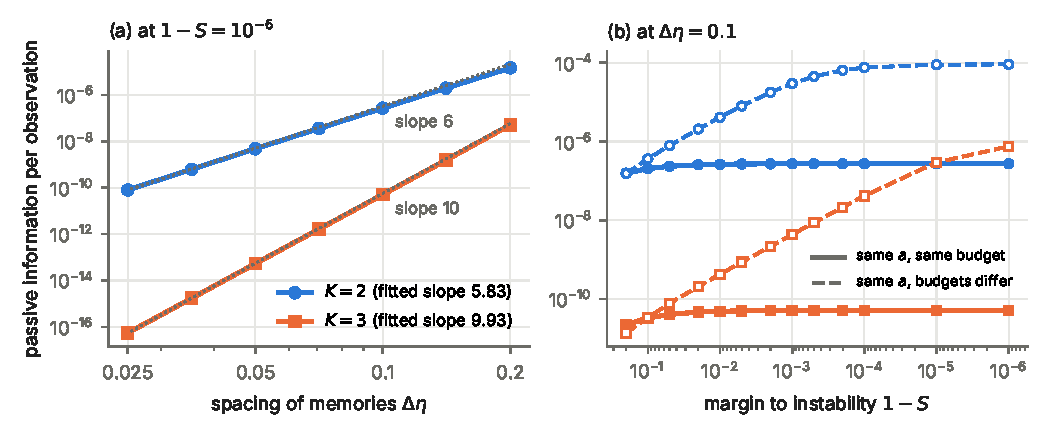
\includegraphics[width=\textwidth]{fig_barrier_admissible.pdf}
\caption{The passive barrier near instability. Both panels show the Gaussian Kullback--Leibler information per observation between the stationary price processes of two populations whose merged measures are the $K$-node Gauss and Gauss--Radau rules on memories spread over $\Delta\eta$ around $0.5$ (total weight $0.3$, impact $\kappa=0.5$). (a)~At a common persistence and a common feedback budget one millionth below instability, the information falls like $(\Delta\eta)^{4K-2}$ (dotted lines). (b)~With a common persistence and a common budget (solid; the Gauss--Radau weights rescaled by a factor $1+O((\Delta\eta)^{2K-1})$), the information stays bounded as the margin $1-S$ shrinks. With a common persistence and no rescaling (dashed), the budgets differ by order $(\Delta\eta)^{2K-1}$; the information then grows roughly like $(1-S)^{-1}$ until the margin reaches that gap, and levels off. Computed from the closed-form spectra.}
\label{n:fig_barrier}
\end{figure}

\paragraph{How large is the barrier?} Table~\ref{n:tab_cal} evaluates the lower bound for particular moment-matched pairs under the listed parameter values and passive Gaussian observation contract. At the illustrative half-lives of 5--9 periods and a daily sampling convention, some pairs require more than $11{,}000$ calendar years to distinguish at the stated error level. This is a worst-case example, not a bound for every population in that range or a fitted market horizon. Smaller lower bounds for more separated pairs do not by themselves establish that the associated sample size is sufficient. Regular non-Gaussian innovation families can retain the exponent under the location-divergence assumptions of \citet[Proposition~S16.2]{niroula2026full}; bounded-support laws are outside that claim. Synthetic groups driven by resampled Bitcoin noise provide an additional numerical check, not a theorem for arbitrary real-market noise.

\begin{table}[t]
\centering
\caption{Years of daily price data below which no test tells the two populations of Theorem~\ref{n:cost}(i) apart with both error probabilities at $5\%$.}
\label{n:tab_cal}
\begin{tabular}{cccrr}
\toprule
& memory rates & half-lives (days) & $1-S=0.1$ & $1-S=10^{-6}$\\
\midrule
$K=2$ & $0.5\pm0.1$ & 0.8--1.4 & 31{,}000 & 23{,}000\\
 & $0.5\pm0.05$ & 0.9--1.2 & $1.8\times10^{6}$ & $1.3\times10^{6}$\\
 & $0.8\pm0.1$ & 1.9--6.6 & 280 & 160\\
 & $0.8\pm0.05$ & 2.4--4.3 & 15{,}000 & 8{,}100\\
 & $0.9\pm0.05$ & 4.3--13.5 & 480 & 230\\
 & $0.9\pm0.025$ & 5.2--8.9 & 25{,}000 & 11{,}000\\
\midrule
$K=3$ & $0.5\pm0.1$ & 0.8--1.4 & $2.0\times10^{8}$ & $1.3\times10^{8}$\\
 & $0.5\pm0.05$ & 0.9--1.2 & $1.9\times10^{11}$ & $1.2\times10^{11}$\\
\bottomrule
\end{tabular}
\par\smallskip
\parbox{\textwidth}{\footnotesize Bound: $n\ge\ln 5/\mathrm{KL}$ observations (Bretagnolle--Huber), with KL the Gaussian information per observation, computed as in Figure~\ref{n:fig_barrier}, at a common persistence and a common feedback budget $S$ (the Gauss--Radau weights rescaled to match the budget), impact $\kappa=0.5$ and feedback share $\kappa\sum_iq_i=0.3$ (total weight $0.6(1-r_c)$ of the Gauss economy at centre rate $r_c$). Memory rates are per day, 252 days a year; for traders whose memories are counted in five-minute periods, with prices recorded every five minutes around the clock, divide by $417$. With non-Gaussian news the bounds can be smaller, by at most the factor $\sigma^2I^*_f$ of Theorem~\ref{n:cost} ($2$ for Laplace news), which can be large for heavy-tailed news. Two significant digits.}
\end{table}

\paragraph{The barrier does not depend on exponential memory.} Exponential memory makes the problem explicit, but the exponent has a more general source. Let each type of trader be indexed by a number $\theta$ in an interval $\Theta$ and trade $f_\theta(h)$ after the public history $h=(x_t,x_{t-1},\ldots)$, where $f_\theta$ is any causal rule: a power-law or hump-shaped memory, a fixed lookback window, a saturating rule, or a learning rule with a fixed tuning parameter. A population is a finite measure $\nu$ on $\Theta$, the weight on each type, and its aggregate flow
\[
F_\nu(h)=\int f_\theta(h)\,\nu(d\theta)
\]
is linear in $\nu$ whatever the rules. Prices follow \eqref{n:eq:model} with $\kappa F_\nu(h_{t-1})$ in place of the feedback term. Theorem~\ref{n:suff} says that $F_\nu$ is all that prices can reveal; the next result says what it costs to read $\nu$ from it.

\begin{theorem}[A lower bound for smooth families]\label{n:univ}
Fix $K\ge2$, a centre type $\theta_c$, a total weight $W>0$ and a spread $\Delta>0$ with $[\theta_c-\Delta,\theta_c+\Delta]\subset\Theta$. Suppose that $\theta\mapsto f_\theta(h)$ has $2K-1$ continuous derivatives at every history, with $|\partial_\theta^{2K-1}f_\theta(h)|\le B(h)$, and that innovations, conditional on the observed past and chosen probe, are independent Gaussian with variance $\sigma^2>0$. Compare records from the same fixed observed initial history (or a common, fully observed initial state law). The observer uses the same predictable policy and independent randomization in both economies.
\begin{enumerate}[label=(\roman*),itemsep=1pt]
\item \emph{Flow gap.} There are two populations $\nu$ and $\nu'$, each with $K$ types in $[\theta_c-\Delta,\theta_c+\Delta]$, positive weights and total weight $W$, at Wasserstein distance $W_1(\nu,\nu')=d_KW\Delta$ for a constant $d_K>0$, whose aggregate flows satisfy, at every history,
\[
|F_\nu(h)-F_{\nu'}(h)|\le\frac{2W}{(2K-1)!}\,B(h)\,\Delta^{2K-1}.
\]
\item \emph{Lower bound.} Suppose $\mathbb E_\nu[B(h_t)^2]\le\bar B^2$ at every date under the specified policy, with $0<\bar B<\infty$. For an asymptotic rate claim, this bound is uniform over the spreads, dates and admissible policies considered. For any probes, none or chosen from the observer's own past and randomization, a record of $T$ periods (for example $N$ reset experiments of length $T/N$) tells $\nu$ from $\nu'$ with both error probabilities below $1/4$ only if
\[
T\ \ge\ \frac{\big((2K-1)!\big)^2}{4\kappa^2W^2\bar B^2}\;\sigma^2\,\Delta^{-(4K-2)}.
\]
\end{enumerate}
\end{theorem}

The proof uses moment cancellation and sequential likelihoods (Supplement Section~\ref{app:univirr}). The two populations are the $K$-node Gauss and Gauss--Radau quadrature rules on the interval, which integrate every polynomial of degree $2K-2$ alike, so a Taylor expansion of $f_\theta$ in $\theta$ leaves only the remainder of order $2K-1$. With Gaussian news, the chain rule for Kullback--Leibler information then charges each period the squared gap between the two populations' predicted flows. Nothing uses exponential memory, linearity in the history, or the structure of the loop, and the same argument covers the observer who only waits. Exponential feedback fits this framework either with $f_r(h)=\sum_jr^jx_{t-j}$ and population measure $M=\sum_iw_i\delta_{r_i}$, or with $f_r(h)=(1-r)\sum_jr^jx_{t-j}$ and activity measure $\sum_iq_i\delta_{r_i}$. The mass $W$ and the Wasserstein loss refer to the chosen parameterization; $w_i=q_i(1-r_i)$. Theorem~\ref{n:cost}(i) supplies explicit constants for its exponential-memory experiment. A shared-leverage saturating family can also fall under the theorem when its derivative-moment condition holds. Distinct leverages lead to a different identification problem (Companion Proposition~\ref{prop:nlcost}).

\citet[Proposition~S29.1]{niroula2026full} gives a conditional matching upper bound in a fixed-history flow experiment under a strong-identifiability condition, which smoothness alone does not deliver. The next theorem proves such a bound for linear memory rules.

\Needspace{6\baselineskip}
\begin{theorem}[Recovery within a shrinking cluster of linear memory rules]\label{n:shape}
Fix known $K\ge2$, $a$, $\kappa>0$, $\theta_c$, $L\ge2K$, and a nonempty compact parameter class
\[
\mathcal Z=\{(s,w):-1\le s_1<\cdots<s_K\le1,\ s_{i+1}-s_i\ge\gamma,
\ \omega_{\min}\le w_i\le\omega_{\max}\},
\]
where $\gamma>0$ and $0<\omega_{\min}\le\omega_{\max}<\infty$ are fixed. Let $g=(g_0,\ldots,g_{L-1})$ be $C^{2K}$ near $\theta_c$, with its derivative vectors of orders $0,\ldots,2K-1$ linearly independent there. The population has kernel $k_m=\sum_iw_i g_m(\theta_c+\Delta s_i)$, with known $\Delta>0$. Observe $N\ge1$ independent copies of its deterministic zero-state unit-impulse response $(h_0,\ldots,h_L)$ plus independent $N(0,\sigma^2 I_{L+1})$ measurement noise, $\sigma>0$.

There are $\Delta_0>0$ and $C<\infty$, depending on this fixed class and response design, such that for $0<\Delta\le\Delta_0$ every exact minimum-distance estimator over $\mathcal Z$ satisfies, with probability at least $1-\delta$, $0<\delta<1$,
\[
\|\hat z-z\|\le C\sigma\big(\sqrt{L+1}+\sqrt{2\log(1/\delta)}\big)
N^{-1/2}\Delta^{-(2K-1)}.
\]
The rank condition holds for $g_m(\theta)=(1-\theta)\theta^m$ at $\theta_c\in(0,1)$ and for $g_m(\theta)=(m+1)^{-\theta}$; taking $\theta_c>1$ in the latter gives summable infinite-memory rules on a sufficiently small neighborhood.
If the class contains the two Gauss--Radau/Gauss configurations with a common positive mass, distinguishing them requires $N\ge c\sigma^2\Delta^{-(4K-2)}$ at errors below $1/4$. Thus, for fixed confidence and sufficiently small fixed accuracy in the weights and rescaled types, the upper and lower orders agree on such a class.
\end{theorem}

The inverse estimate is global over the fixed separated class $\mathcal Z$, within a sufficiently small physical cluster. It does not establish global identification over an unrestricted type interval or over unknown numbers of types. Its constants can deteriorate as $\gamma$ or $\omega_{\min}$ tends to zero. The estimator is an exact global minimizer over $\mathcal Z$, which is not convex, and the theorem gives no algorithm that finds it. The observation law is explicitly a noisy deterministic-response experiment; identifying it with passive process-noise data would require a separate argument. \citet[Proposition~S29.1]{niroula2026full} remains useful for other response families, including nonlinear ones for which this rank argument supplies no upper bound. Supplement Section~\ref{app:incoming} gives the inverse proof. The optimizer simulation in the repository starts at the true parameter and is interpreted only as a local conditioning diagnostic, not as a deployable global recovery algorithm.

\section{What a record reveals}\label{n:irr_sec}

The forecasting target is the pricing error $x_t$ in \eqref{n:eq:model}. We assume it is observed by the forecaster. Observing a traded price $p_t=x_t+f_t$ alone does not generally reveal $x_t$. The forecast benchmarks take $q_i\ge0$, $0<r_i<1$, $\kappa>0$, $S<1$ and no probes, with boundary cases stated explicitly. The pairwise detection comparison separately allows predictable probes. The results use different initialization and decision regimes.


\begin{theorem}[Pairwise detection and forecast mismatch]\label{n:dual}
Consider two specified causal aggregate maps $F,F'$ with the same known $a,\kappa$, common observed initial information, independent $N(0,\sigma^2)$ innovations, and a common predictable probe policy including the same independent randomization. Assume the required squared mean gaps are integrable. For a record of $T$ subsequent innovations, let
\[
V_t=\kappa^2\mathbb E_P[(F(h_t)-F'(h_t))^2],\qquad
\Lambda_T=\sigma^{-2}\sum_{t<T}V_t.
\]
Then $V_t$ is the excess mean squared forecast error of using the alternative conditional mean on the true record, and
\[
\mathrm{KL}(P_T\Vert P'_T)=\Lambda_T/2.
\]
Both testing errors can be below $1/4$ only if $\Lambda_T>1$.
For a countable set of candidate record densities with prior mass $\pi_*>0$ on the truth, the Bayesian mixture also satisfies the one-sided pathwise bound
\[
\log p_*(X_{1:T})-\log q(X_{1:T})\le\log(1/\pi_*).
\]
\end{theorem}

This is the Gaussian chain rule and the standard mixture likelihood bound, applied to the market experiment \citep{dawid1984,vovk2001}. Given three probability facts that enter as explicit hypotheses (the one-step Gaussian divergence, the chain rule over the record and Pinsker's inequality), the algebra of the theorem is machine-checked (\nolinkurl{dual_end_to_end}, \nolinkurl{excess_forecast_error}, \nolinkurl{mixture_bound}). It identifies a pairwise forecast mismatch with a directional information divergence. It does not identify total information about an unrestricted population, prove that every kernel is cheaply estimated, or make a failed detection test evidence of a small KL divergence. The test condition is necessary, not sufficient. The mixture bound is an upper bound on regret, not an absolute difference of log scores; it requires positive prior mass on the true candidate.

\paragraph{Forecasting without composition.} Composition is not needed to forecast the pricing error either. With known parameters, the price record and the class records give the same optimal forecast; for a fixed unknown population, a fitted autoregression of order $\log T$ attains the known-population forecast up to excess risk of order $\sigma^2\log T/T$, and a Bayesian autoregression has a cumulative log-loss bound that is uniform over stable populations (Supplement Theorems~\ref{n:irr} and~\ref{n:uniformlog}). What a supervisor cannot get from prices is therefore not a better forecast but the attribution that a targeted policy needs.

\section{Who needs composition, and what disclosure buys}\label{n:sup}

\begin{proposition}[Market-wide versus targeted action]\label{n:target}
Let $q_i\ge0$, let the market be stable with $(a,\kappa)$ known, and let a supervisor need the feedback budget below a ceiling $\bar s$, with $a<\bar s<1$.
\begin{enumerate}[label=(\roman*),itemsep=1pt]
\item \emph{Market-wide.} Scaling all feedback activity by $\theta$ meets the ceiling exactly when $a+\theta(S-a)\le\bar s$. This depends on the population only through $S$, and so only through the kernel.
\item \emph{Targeted.} Halting the largest group does not. For every $K\ge2$ there are two populations whose merged measures have the same moments of order $0,\ldots,2K-2$, so that their budgets differ only by order $(\Delta\eta)^{2K-1}$, while their largest groups differ by a fixed amount, so that for a range of ceilings the halt meets the ceiling in one and not the other. Making this decision from $N$ reset records with both errors at most $1/4$ needs $N\ge c\,\sigma^2(\Delta\eta)^{-(4K-2)}$.
\end{enumerate}
\end{proposition}

Part~(i) is Supplement Proposition~\ref{prop:target}(i). Part~(ii) is Supplement Proposition~\ref{prop:targetK}; its pair comes from a family of quadrature rules whose weights are the values of one function at their nodes (Supplement Lemma~\ref{lem:everyK}).

\paragraph{What setting a uniform cut from prices requires.} Part~(i) takes the persistence $a$ as known, and that is a restriction on the population: a group with memory zero acts exactly like persistence (Supplement Theorem~\ref{thm:merged}(i)), so knowing $a$ amounts to assuming that every memory exceeds some $\underline r>0$, or to knowing which part of the response at the first lag is feedback. The budget also needs a bound on memory. It is the linear question $g(r)=1/(1-r)$, and by Theorem~\ref{n:questions}(iii) a group with memory close to one and negligible weight can move it at bounded divergence unless memories are bounded by some $\bar r<1$. Under both restrictions the budget is learned at nearly the parametric rate (Theorem~\ref{n:questions} and the paragraph after it); without them, the uniform cut inherits part of the composition problem. The instrument must also scale feedback traders while sparing arbitrageurs and dealers. Real instruments, such as transaction taxes, minimum resting times and order-to-trade limits, act with an incidence $\theta(r)$ that varies with the trader's horizon, so their effect on the budget is governed by $\int\theta(r)(1-r)^{-1}\,dM(r)$. Theorem~\ref{n:questions} sorts them: an incidence that is smooth in memory is cheap to evaluate from prices, and one that singles out a narrow band of memories is not.

\begin{corollary}[Expected loss from a weakly identified intervention]\label{n:decisionloss}
Consider the pair in Proposition~\ref{n:target}. In economy 0 a halt of the largest verified class misses the prudential ceiling, while a common reduction meets it; in economy 1 both meet it. Let the loss of the unsuccessful halt in economy 0 be $b>0$, and the loss of an unnecessarily common restriction in economy 1 be $c>0$, with the other two losses zero. For equally likely economies and public-record laws $P_0,P_1$, every choice rule has average loss
\[
R\ \ge\ \frac{\min(b,c)}{2}\{1-\operatorname{TV}(P_0,P_1)\}
\ \ge\ \frac{\min(b,c)}{2}\big[1-\sqrt{\mathrm{KL}(P_0\Vert P_1)/2}\big]_+.
\]
If the specified price experiment has $\mathrm{KL}(P_0\Vert P_1)\le C T\Delta^{4K-2}$, achieving $R\le\epsilon\min(b,c)$, $0<\epsilon<1/2$, requires
$T\ge 2(1-2\epsilon)^2/(C\Delta^{4K-2})$.
For independent Gaussian tagged measurements with common covariance $\tau^2I$, mean difference $d\ne0$ and $N$ repetitions, the likelihood-ratio rule instead has
\[
R_{\rm tag}\le \tfrac12\max(b,c)\exp\{-N\|d\|^2/(8\tau^2)\}.
\]
\end{corollary}

This is a decision-theoretic consequence of the hard pair, not a new statistical lower-bound method. The losses are specified primitives, not estimated welfare effects. The tagged statement assumes a verified executable class identity and means known under the two hypotheses. It does not establish optimal disclosure in an unrestricted market. The proof and a stable two-class example are in Supplement Section~\ref{app:revisiondecision}.

\begin{theorem}[Without tags, uniform policies are minimax]\label{n:minimax}
Let class $d$ contribute $H_d$ to the feedback budget, $U=\sum_dH_d$, and let a policy scale the feedback of the class carrying label $c$ by $\theta_c$, at cost $C(\theta)$. The resulting budget is $S'_\pi=a+\sum_c\theta_cH_{\pi(c)}$, where $\pi$ is the unknown assignment of labels to classes, and its loss is $\ell(S'_\pi)$. If $\ell$ is convex and $C$ is convex and unchanged when labels are permuted, the uniform policy that scales every class by $\bar\theta=K^{-1}\sum_c\theta_c$ has a budget $a+\bar\theta U$ that does not depend on $\pi$, and
\[
\ell(a+\bar\theta U)+C(\bar\theta\mathbf 1)\ \le\ \frac1{K!}\sum_\pi\ell(S'_\pi)+C(\theta)\ \le\ \max_\pi\ell(S'_\pi)+C(\theta).
\]
Labels do not enter prices, so no record distinguishes labellings; the uniform policy does at least as well as $\theta$ against the worst labelling (it is minimax) and on average over labellings (it is Bayes under an exchangeable prior).
\end{theorem}

The proof averages over labellings. Every label is carried by every class equally often, so the average budget is $a+\bar\theta U$ and the average relabeled policy is $\bar\theta\mathbf 1$; Jensen's inequality for $\ell$ and for $C$ gives the first inequality, and an average is at most a maximum. The theorem is machine-checked in full (\nolinkurl{PublicationRevision10.lean}). The argument is the finite-group case of the Hunt--Stein theorem \citep[Chapter~8]{lehmann2005}. Because the law of the record does not depend on the labelling, it applies record by record, so it also covers policies that depend on the record. The comparison with the worst labelling, $\ell(a+\bar\theta U)+C(\bar\theta\mathbf 1)\le\max_\pi\ell(S'_\pi)+C(\theta)$, also holds when $\ell$ and $C$ are only quasi-convex, as is the loss of missing a ceiling: replace Jensen's inequality by $\ell(\sum_\pi\lambda_\pi x_\pi)\le\max_\pi\ell(x_\pi)$. The comparison with the average does not extend, and the quasi-convex case is not machine-checked. Tags break the symmetry the proof uses: with verified labels the supervisor can tailor the policy to each class, and the gain from doing so is the value of tags studied in Theorem~\ref{n:disc} and Proposition~\ref{n:relabel}. A single halt shows the size of the gap.

\begin{corollary}[What a halt guarantees]\label{cor:robustuniform}
In the setting of Theorem~\ref{n:minimax}:
\begin{enumerate}[label=(\roman*),itemsep=1pt]
\item For every label $F$, halting the class labelled $F$ is guaranteed to lower the budget only by $\min_cH_c$, and some labelling consistent with the record attains this.
\item A uniform cut to the fraction $\theta=(\bar s-a)/(S-a)$ brings the budget exactly to the ceiling $\bar s$ in every population with budget $S$, and no policy that meets the ceiling removes less feedback than $S-\bar s$.
\end{enumerate}
So a halt of one class meets the ceiling with certainty only if $\min_cH_c\ge S-\bar s$, while the uniform cut always meets it with the least removal. Without tags, the guarantee of a targeted halt is set by the weakest class, not the one targeted.
\end{corollary}

Tags change the answer group by group.

\begin{theorem}[What tags buy, in minimax terms]\label{n:minimaxtags}
Let verified tags split the classes into groups $g=1,\ldots,G$, so that the record identifies each class's group but cannot rule out relabelings within a group. Let $\ell$ be convex and $C$ convex and unchanged by relabelings within groups. The policy that scales every class of group $g$ by the group's average intensity $\bar\theta_g$ has the budget $a+\sum_g\bar\theta_gU_g$, with $U_g=\sum_{d\in g}H_d$, under every labelling consistent with the record, and it does at least as well as $\theta$ against the worst such labelling. The minimax supervisor therefore chooses one intensity per tagged group, and the value of tags is
\[
V=\min_{\bar\theta}\,\max_\pi\{\ell(S'_\pi)+C\}-\min_{(\bar\theta_g)_g}\max_\pi\{\ell(S'_\pi)+C\}\ \ge\ 0,
\]
the gain from tailoring intensities across verified groups. With a single group, $V=0$ and Theorem~\ref{n:minimax} is recovered; with every class its own group, $V$ is the full value of targeting.
\end{theorem}

The proof restricts the averaging of Theorem~\ref{n:minimax} to relabelings within groups: within a group, every label is carried by every class of the group equally often, so averaging replaces each intensity by its group mean and the budget by $a+\sum_g\bar\theta_gU_g$. It is machine-checked in full (\nolinkurl{PublicationRevision11.lean}). This is the decision-theoretic counterpart of Theorem~\ref{n:disc}: tags are worth what they let a supervisor tailor, and Proposition~\ref{n:relabel} prices how far relabeling erodes that.

\begin{figure}[tb]
\centering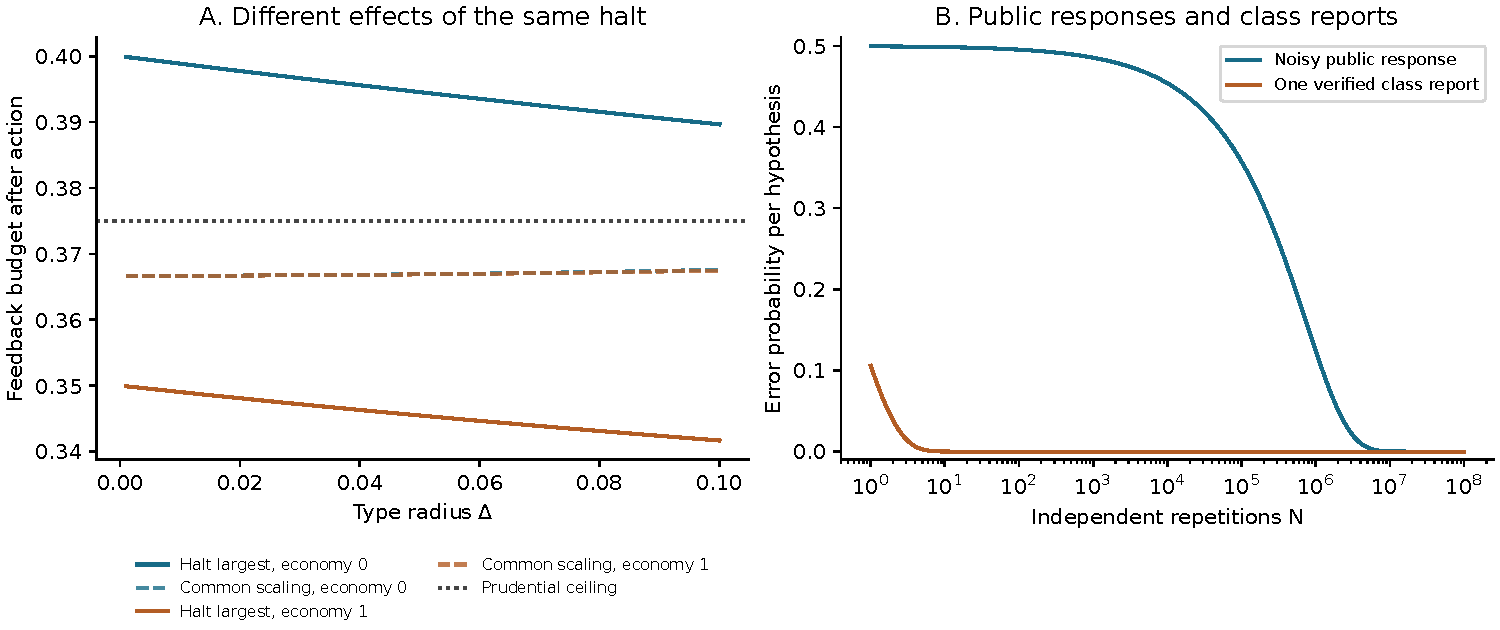
\includegraphics[width=\textwidth]{fig_intervention_revision.pdf}
\caption{\textbf{Intervention choice and an illustrative information comparison.} Panel A uses the two-class construction in Supplement Section~\ref{app:revisiondecision}, with $a=0.3$, $\kappa=0.5$, $W=0.2$ and $r_c=0.5$. A ceiling of $0.375$ separates the post-halt budgets while common scaling meets it in both economies. Panel B fixes $\Delta=0.05$ and compares exact likelihood-ratio errors for two known hypotheses. Each repetition measures 30 deterministic impulse-response coordinates with independent Gaussian measurement standard deviation $0.01$; the class report measures $\kappa w_1$ with the same standard deviation. The calculated requirements for 5\% error are about $2.03\times10^6$ public-response repetitions and two class reports. These are assumptions of an illustrative measurement experiment, not a passive-innovation model, feasible live reset policy or market calibration.}
\label{fig:revisiondecision}
\end{figure}

\begin{theorem}[Value of class-tagged disclosure]\label{n:disc}
Suppose that, in addition to prices, the observer receives each class's flow with Gaussian measurement noise. On the rich class of Theorem~\ref{n:cost}(ii), the number of experiments needed to recover the weights falls from order $(\Delta\eta)^{-(4K-2)}$ to a bound that does not depend on $\Delta\eta$. For the rates it falls to order $(\Delta\eta)^{-2}$.
\end{theorem}

This is Supplement Theorem~\ref{thm:discvalue}; Supplement Proposition~\ref{prop:tagged} gives the regression that achieves it, one class at a time, with a variance that depends only on that class. Supplement Proposition~\ref{prop:choice} says when a supervisor should pay for such an audit trail: when the algorithms to be told apart are close enough that prices take too long, but not so close that even tagged data cannot help, and when the trail covers enough markets to recover its fixed cost.

Three further results are in the supplement. Tagging $m$ of the $K$ groups lowers the exponent of the composition cost by four per tag, and tagging all but one memory class removes the spacing penalty for weight recovery (Supplement Theorem~\ref{thm:partial}). Pooling price records from $D$ markets in which the same algorithms trade in different proportions lowers the exponent to $2(K-1+\lceil K/D\rceil)$ near generic configurations, so cross-market surveillance is a partial substitute for tagging (\citealp[Theorem~S5.5]{niroula2026full}). Monitors built on eigenvalues and second moments of prices are not uniformly safe (\citealp[Theorem~S26.1]{niroula2026full}).

The results so far take the groups' rules as given. A group that expects to be targeted can change its rule toward a population that is targeted less often: whatever the probes and record length, it is then targeted with probability at most $\alpha+C_0/P$, where $\alpha$ is that population's targeting probability, $C_0$ the cost of the change and $P$ the cost of being targeted (Supplement Proposition~\ref{prop:hiding}). A class tag is attached to the account, so changing the trading rule does not remove it. Activity can, however, be routed through accounts that carry another label. The next result solves the disclosure game when it can.

\begin{proposition}[Disclosure when labels can be gamed]\label{n:relabel}
Fix one supervisory cycle. A share $\chi\in(0,1)$ of feedback activity belongs to a class $H$ and the rest to a class $S$. Each retained unit of activity has net social value $n_H<0<n_S$, and $H$ traders gain $b_H>0$ per retained unit. Without disclosure the only restriction is a uniform retention $x\in[0,1]$ of all activity. With class tags the supervisor sets a retention $y$ for the $H$ label and $x\ge y$ for the $S$ label, and $H$ traders may route a share $z\in[0,1]$ of their activity through $S$ labels at resource cost $\gamma z^2/2$ per unit of $H$ activity, $\gamma>0$. An audit trail that links accounts to owners prevents relabeling. Write $a=-n_H$, $m=\chi n_H+(1-\chi)n_S$, $s=(1-\chi)n_S$ and $g=\gamma/\{b_H(2a+b_H)\}$.
\begin{enumerate}[label=(\roman*),itemsep=1pt]
\item $H$ traders route $z^*=\min\{1,\,b_H(x-y)/\gamma\}$ through $S$ labels.
\item Without disclosure the welfare is $\max\{0,m\}$; with an audit trail it is $s$, before its cost. With class tags the optimal policy, and its gain $V_C$ over the uniform cut, are as follows. If $m\ge0$: $x=1$, the label gap is $x-y=\min\{1,ag\}$, and $V_C=\chi a^2g/2$ when $ag\le1$, $V_C=\chi a-\chi/(2g)$ otherwise. If $m<0$: $y=0$, $x=\min\{1,sg/\chi\}$, and $V_C=s^2g/(2\chi)$ when $sg\le\chi$, $V_C=s-\chi/(2g)$ otherwise. In every case the equilibrium hiding share lies strictly between $0$ and $1$.
\item $V_C$ is continuous and strictly increasing in $\gamma$, tends to $0$ as $\gamma\to0$ and to the audit trail's gain $V_A=s-\max\{0,m\}$ as $\gamma\to\infty$, and $V_C<V_A$ for every $\gamma$. With fixed costs $F_C\le F_A$ of class tags and of the audit trail, the audit trail is preferred to class tags exactly when $F_A-F_C<V_A-V_C(\gamma)$, that is, when $\gamma$ lies below a threshold.
\end{enumerate}
\end{proposition}

Three consequences follow. First, cheap relabeling restores observational equivalence in equilibrium: as $\gamma\to0$ the optimal tag policy converges to the uniform cut and class tags are worth nothing, so the identification problem of Section~\ref{n:cost_sec} reappears as an incentive problem. Second, the optimal targeted restriction is partial. When uniform retention is worthwhile ($m\ge0$), the supervisor leaves the harmful label partly open, with a label gap proportional to the relabeling cost and decreasing in the restricted traders' private gain; when it is not ($m<0$), it also restricts the benign label, because that label is the hiding channel. Third, an audit trail that links accounts to owners keeps its full gain at every $\gamma$, so its advantage over class tags is largest where relabeling is cheapest. This ranking is built in, because the audit trail is assumed not to be gameable. What it needs is a stable link from accounts to an owner, which can be pseudonymous: the Consolidated Audit Trail, for example, keeps consistent anonymized customer identifiers after the 2025 exemption from reporting names, addresses and years of birth \citep{sec2025cat}. Labels that firms assign to their own algorithms are the gameable kind. That a principal should rely less on a signal that agents can manipulate is close to \citet{frankel2022} and \citet{perezrichet2022}. Proposition~\ref{prop:choice} holds behaviour fixed across regimes; here it responds to them. The closed forms use linear values and a quadratic concealment cost, as in the costly-state-falsification literature \citep{lackerweinberg1989,crockermorgan1998}. The limits do not: with concave private payoffs, any convex concealment cost and any Lipschitz welfare of effective retentions, including an externality that depends on aggregate feedback, class tags are worth only the value of the coarse partition when relabeling is cheap, approach the audit trail's value when it is expensive, and are worth nothing if every class can reach every label (Supplement Theorem~\ref{thm:relabelgeneral}). The model has one cycle and enforced retentions. The proof is in Supplement Section~\ref{app:relabel}. Its steps, including the case analysis and the dominance of complete pooling, are checked in Lean~4, and its closed forms also by brute force. With many classes the same logic holds channel by channel: as relabeling becomes cheap, class tags are worth only what a coarser partition is worth, in which each class receives the best retention among the labels it can reach (Supplement Proposition~\ref{prop:relabelK}). If labels are assigned from measured memory and shifting it costs the square of the shift, behaviour-based tags lose their value as memories approach each other, the same limit in which Theorem~\ref{n:cost} makes prices uninformative about composition (Supplement Corollary~\ref{cor:relabelspacing}). At the optimum the share of restricted activity that hides does not depend on the cost of hiding, and the more profitable the restricted activity, the milder the optimal restriction and the less class tags are worth (Supplement Corollary~\ref{cor:relabelstatics}).

\paragraph{Surveillance when algorithms can hide.} The results so far take memories as given. An algorithm that expects to be targeted once identified can trade more like its neighbour, at a cost to its own strategy. The next result gives what the supervisor learns when the algorithm best-responds to a fixed test.

\begin{theorem}[The surveillance paradox]\label{n:paradox}
An untagged group chooses the distance $\delta\in[0,\delta_0]$ between its memory and its neighbour's; the neighbour and all other groups stay where they are. The supervisor tests the null that the group trades like its neighbour (one group in place of the two, with unknown memory and weight) at level $\alpha$ under every economy in the null. Detection triggers an inquiry that costs the group $L$, and moving costs it $k(\delta_0-\delta)^2$, with $\delta_0,k,L>0$. With $N$ observations, let $J$ be the divergence from the record with the group at distance $\delta$ to the closest record in the null. We take its leading order, $J=cN\delta^n$ with $n>2$; for a group and its neighbour, $n=4$. The test is unbiased, and its detection probability depends on $\delta$ only through $J$: it is $P_{\rm d}(J)\ge\alpha$. Let $\delta^*$ be an optimal distance and $J^*=cN\delta^{*n}$.
\begin{enumerate}[label=(\roman*),itemsep=1pt]
\item \emph{Hiding is never complete.} Against every such test, $\delta^*>0$, and $\delta^{*\,n-2}\ge2k^2\delta_0^2/(2^nL^2cN)$ whenever $\delta^*\le\delta_0/3$.
\item \emph{A good test forces crowding.} Suppose the test's power satisfies $P_{\rm d}(J)-\alpha\ge\beta\min\{\sqrt J,\sqrt{\bar J}\}$ and the stakes are high, $L\beta\sqrt{\bar J}>k\delta_0^2$. Then, for every $N$,
\[
\delta^{*\,n-2}\le\frac{4k^2\delta_0^2}{L^2\beta^2cN}.
\]
\item \emph{More data, less information.} Against such a test, for all large $N$, $\delta^*$ is of exact order $N^{-1/(n-2)}$ and the supervisor's information $J^*$ is of exact order $N^{-2/(n-2)}$: like $N^{-1}$ for a group and its neighbour. The detection probability tends to $\alpha$, and the group's distortion cost $k(\delta_0-\delta^*)^2$ tends to $k\delta_0^2$.
\item \emph{Tags reverse it.} With a class tag, detection does not depend on $\delta$, so $\delta^*=\delta_0$, and the supervisor learns the group's rule from its tagged flow (Theorem~\ref{n:disc}).
\end{enumerate}
\end{theorem}

The exponent depends on what the supervisor knows. The record does not say which nearby memory is the neighbour's, so the null is composite. A single group with the pair's total weight and mean memory matches the kernel up to the spread of the two memories, which is of order $\delta^2$ in the kernel and $\delta^4$ in the divergence (Supplement Theorem~\ref{prop:passive}(i); computed from the spectra, the slope is $4.1$, Supplement Section~\ref{app:paradox}). A supervisor that knew the neighbour's memory and both weights would face a simple null with $n=2$; then, against the Gaussian test with high stakes, hiding is complete once $N$ is large, and the record carries no information about the group. In the limiting Gaussian experiment, the one-sided test in the direction orthogonal to the null satisfies (ii) with $\beta=\sqrt2\,\phi(z_\alpha)$ and $\bar J=z_\alpha^2/2$.

Without tags, each new observation is more than offset by the crowding it provokes: doubling the data shrinks the optimal distance by the factor $2^{-1/(n-2)}$, and the information falls. Against a group that best-responds, supervision does not converge to knowledge of composition however long the record. The group pays for its invisibility with a distorted strategy, at a cost approaching $k\delta_0^2$. Whether this is a failure depends on what the supervisor wants. If the conduct at $\delta_0$ is what it fears, the crowding is deterrence; what fails is learning, not necessarily welfare. This is the tension between acting on market information and preserving it \citep{bond2010,bond2015}, here for information about who trades rather than about fundamentals; \citet{frankel2019} study how manipulation muddles a signal. The loss $L$ stands for the inquiry that detection triggers, for example a request to brokers for account records; without such an inquiry, detection would have no consequence (Theorem~\ref{n:minimax}). Supplement Proposition~\ref{prop:hidegame} bounds detection for any power function and lets several groups move at once; Theorem~\ref{n:paradox} gives the rate for one group. The proof is in Supplement Section~\ref{app:paradox}; its deterministic steps are checked in Lean~4 and its rates numerically.

\begin{table}[t]\centering\footnotesize\setlength{\tabcolsep}{4pt}
\caption{Tagged rules in Taiwan, 2013--2016 (stock fixed effects; 95\% date-block bootstrap intervals). $r_c$: persistence; $w_c$: response to the previous day's price deviation; $H_c=\kappa w_c/(1-r_c)$: the fall in the feedback budget if class $c$'s feedback is halted.}\label{tab:barrier}
\begin{tabular}{lccc}\toprule
Class & $r_c$ & $w_c$ & $H_c$\\\midrule
Foreign investors & $0.35$ [$0.31$, $0.38$] & $0.24$ [$0.21$, $0.27$] & $0.0014$ [$0.0012$, $0.0016$]\\
Investment trusts & $0.41$ [$0.39$, $0.43$] & $0.066$ [$0.057$, $0.076$] & $4.2\times10^{-4}$ [$3.3\times10^{-4}$, $5.3\times10^{-4}$]\\
Dealers & $0.33$ [$0.22$, $0.42$] & $-0.022$ [$-0.028$, $-0.017$] & $-1.3\times10^{-4}$ [$-1.8\times10^{-4}$, $-8.2\times10^{-5}$]\\
\midrule
\multicolumn{4}{l}{Impact of lagged flow $\kappa$: $0.0038$ [$0.0032$, $0.0044$]; price persistence $\sum_ja_j$: $0.97$.}\\
\bottomrule\end{tabular}\end{table}
\paragraph{The barrier in a real market.} Taiwan's exchange reports each day's net buying in every listed stock by three classes: foreign investors, investment trusts and dealers. Over 2013--2016 (300 stocks, 270{,}060 stock-days) we estimate each class's rule from its own flow and the market's response to flow from prices (Table~\ref{tab:barrier}). We then ask what a supervisor who sees only prices could learn, granting that supervisor the market's impact function and the law of non-feedback order flow, so that only the composition is unknown. \emph{First, prices separate the classes slowly.} Against the closest single-memory population, in which the three classes share one decay, a stock-day of prices carries $1.7\times10^{-12}$ nats and a stock-day of tagged flows $8\times10^{-7}$, $4.7\times10^{5}$ times more. Before any 5\% test could reach 80\% power, prices alone need at least $2.7\times10^{9}$ years of one stock, or $9.1\times10^{6}$ years of all 300 stocks treated as independent; the tagged record needs at least $5{,}738$ years of one stock. \emph{Second, prices cannot fix a targeted halt.} With tags, foreign feedback contributes $0.0014$ to the feedback budget (95\% interval [$0.0012$, $0.0016$]), so halting it changes the budget by minus that amount. The compositions that the whole panel record cannot tell apart, in the sense that no test exceeds its size by more than 0.10, imply contributions from $-0.028$ to $0.028$; even with each class's contribution capped at twice the largest estimated one, from $-0.0027$ to $0.0027$. However long the record, relabeling alone leaves $0.0014$, $4.2\times10^{-4}$ and $-1.3\times10^{-4}$ all possible. \emph{Third, the uniform cut is fixed by prices.} Over the same compositions, the effect of cutting all feedback lies between $0.0014$ and $0.0019$. These are calibrations of Theorems~\ref{n:cost} and~\ref{n:dual} at the tagged responses, not tests. The registered Taiwan test (Supplement Section~\ref{sec:scope}) did not establish that those responses are feedback rather than prices revealing past flow. The protocol was fixed before the run (\nolinkurl{P1M_measurement_protocol.md}); its deterministic steps are checked in Lean~4 (\nolinkurl{PublicationRevision7.lean}) and the pre-specified sensitivity runs are in Supplement Section~\ref{app:barrier}. Both record lengths compare feedback rules with each class's non-feedback flow held at its estimated law; with tags, each class's contribution is estimated directly, with the intervals of Table~\ref{tab:barrier}. The barrier is this large partly because lagged institutional flow moves prices little ($\kappa=0.0038$): the three classes together contribute $0.0017$ to a feedback budget of $0.97$.

\paragraph{What the calibration shows and what it does not.} Four qualifications apply. First, the targeted range fills the box by construction. Two classes can share one memory with large weights of opposite sign, which leaves the aggregate kernel unchanged, so the range is set by the cap on each class's contribution, not by the data. Weights restricted to one sign would exclude these compositions; we have not computed the range under that restriction. The exact barrier, the relabeling set, does not depend on the cap. Second, the tagged intervals assume that each class's feedback decays at the persistence of its own flow, while the price-only comparisons let feedback memory vary with non-feedback flow held fixed; under the second model, tagged flows carry little information about feedback memory (the $5{,}738$ years above). Third, the uniform cut is fixed by prices only because the supervisor is granted the price persistences $a_j$, the impact $\kappa$ and the non-feedback law, all estimated with the tagged flows. With feedback contributing $0.0017$ to a budget of $0.97$ and memories near $0.35$, separating the two from prices alone is the problem that Proposition~\ref{n:target} assumes away (see the paragraph after it). Fourth, the record lengths treat the 300 stocks as independent, which is generous to prices; the bootstrap resamples dates because they are not independent. Positive feedback in foreign investors' daily flows, and the difficulty of separating it from prices responding to flows, are documented for Taiwan and other markets \citep{froot2001,griffin2004,richards2005}. The dealers' estimated weight is negative, so the calibrated economy lies outside the positive class of Sections~\ref{n:cost_sec}--\ref{n:sup}; the computations here (Whittle rates, Pinsker's inequality, relabeling) do not need positivity.

\section{Scope and conclusion}\label{n:concl}

\paragraph{Drift and position limits.} A group that expects to be targeted can crowd its memory toward its neighbour's, which tags tied to accounts prevent (Supplement Proposition~\ref{prop:hidegame} and Theorem~\ref{n:paradox}). The full working paper \citep{niroula2026full} adds two extensions. If the population drifts by at most $v$ per period, its weights can be tracked with error of order $\min\{1,(\sigma^2v(\Delta\eta)^{-(4K-2)}/n)^{1/3}\}$ and no better, while market-wide quantities are tracked at the cube-root rate whatever the spacing. With hard position limits, populations with the same kernel give identical paths until a limit is reached, while probes that push traders to their limits identify the signed capacity measure. How close traders are to their limits, which decides whether a breach cascades, leaves no trace in calm prices.


\paragraph{Evidence.} The contribution is theoretical. Supplement Section~\ref{sec:scope} reports the registered Taiwan and Binance tests with their readouts and proxy limitations. The registered forecast test on Binance perpetual futures (P1F) was void in its first window, because the archive lacked the trader-class fields its universe rule requires; its replacement window runs from 16 November 2026 to 14 January 2027 and cannot be analysed before 16 January 2027. A second amendment, registered on 20 November 2026 before any window file was read, removes label leakage at the boundary between the training and evaluation halves. A registered account-level test on Hyperliquid, where every trade carries account addresses (H1), is collecting data; it opens no earlier than 10 December 2026, and only if at least 20 coins reach 30 valid days by 31 January 2027. Neither supplies a result here. The local validation report separates recomputed synthetic checks, formal proof checks, inherited empirical readouts and pending studies.

The sufficiency results hold whenever aggregate feedback flow is a causal function of public signals; the kernel is the sufficient object when that function is linear, and $\nu$ when it saturates as in \citet[Section~S6]{niroula2026full}. The explicit identification results and the matching upper bounds need linear rules with exponential memory; the lower bound on the cost of composition holds for smooth families under the common-initialization and uniform derivative-moment conditions (Theorem~\ref{n:univ}), and its attainment needs a strong-identifiability condition (\citealp[Proposition~S29.1]{niroula2026full}). For general rules, prices identify the aggregate flow map and the lower bounds still hold (\citealp[Theorem~S6.7]{niroula2026full}), and for rules within a bounded distance of linear, such as dead bands, large probes identify composition (Companion Proposition~\ref{prop:deadband}); for saturating families, probes that push traders toward their limits identify the signed capacity measure at the parametric rate, and composition costs the linear amount when groups share a leverage but an amount independent of their memory separation when leverages differ (Companion Proposition~\ref{prop:nlcost}); for some nonlinear families composition is not identified at all. For linear rules with general completely monotone memory the minimax accuracy is of order $1/\log(N/\sigma^2)$ (\citealp[Theorem~S18.2]{niroula2026full}). Simulations of saturating, adaptive and neural trading rules show where the linear theory holds and where it fails (Companion Section~\ref{sec:learners}). The passive bounds are stated for Gaussian news, the least favourable case (\citealp[Proposition~S16.2]{niroula2026full}); news with bounded support is not covered. Traders who learn from public data, their own trades and private randomness are covered for what prices reveal: prices identify their aggregate flow kernel and nothing finer, and linear learners whose parameters drift are tracked below the speed limit of \citet[Theorem~S15.1]{niroula2026full} (Companion Proposition~\ref{prop:learners}). A group that chooses its rule against an insider becomes a momentum trader that rides on her information, and its choice is still summarized by the kernel (Companion Proposition~\ref{prop:insidergame}).

\paragraph{Implications and limits.} A uniform scaling of fixed positive feedback activity can be evaluated from the aggregate budget. A restriction on one class can require information that an otherwise informative public record does not supply precisely. This is a statement about the specified interventions and losses; it does not make every market-wide policy identifiable or every targeted policy infeasible. Class identifiers must correspond to executable accounts, reports have noise and costs, and strategic responses can alter the counterfactual. Proposition~\ref{n:relabel} quantifies one such response: class tags are worth only as much as relabeling costs, while owner-linked audit trails are not exposed to it. The companion work studies related safety decisions. A direct empirical test would measure an externally documented class-specific intervention and evaluate predictions fixed before it occurs. The present public-data forecast comparisons do not supply that causal test.

\subsection*{Declarations}

\paragraph{Author contributions.} Pratik Niroula: conceptualization, methodology, formal analysis, software, investigation, data curation, writing (original draft). Prashant Niroula: validation (verification of the proofs, the Lean~4 formalizations and the empirical calculations), writing (review and editing). Sujan Khatiwada: validation (verification of the proofs, the Lean~4 formalizations and the empirical calculations), writing (review and editing). All authors approved the final manuscript.

\paragraph{Funding.} This research received no external funding.

\paragraph{Competing interests.} The authors declare no competing interests.

\paragraph{Data availability.} All data are public. The Taiwan test uses the Taiwan Stock Exchange's daily reports of trading by the three major institutional investors (T86), closing quotes (MI\_INDEX), ex-rights and ex-dividend adjustments (TWT49U) and market totals (FMTQIK), from \url{https://www.twse.com.tw}. The Binance test uses daily files of five-minute candles and trading metrics (including open interest) for USD-margined perpetual futures from the Binance public data archive (\url{https://data.binance.vision}). The registered specifications, amendments, executors, notebooks, result files and test-unlock counters are in the public repository.

\paragraph{Code availability.} The baseline code, Lean~4 proofs and result files are available at \url{https://github.com/Pratikn03/Fianince}.

\paragraph{Ethics approval.} Not applicable. The study uses only public market data and involves no human participants or personal data.

\paragraph{Related manuscripts.} This article grows out of \citet{niroula2026a}, an earlier working paper of the same authors on the same model. It cites that paper only for results not reproduced here: simulations, test reports, the account-level cost of probing, an upper bound for the memory distribution and the rate for completely monotone memory. \citet{niroula2026c} collects companion results on breaches and nonlinear rules. \citet{niroula2026full} is the full working paper of this article, with every supplementary result.

\paragraph{Declaration of generative AI and AI-assisted technologies.} During the preparation of this work the authors used large language model systems (Claude, ChatGPT/Codex and Gemini) for literature search, code development, numerical checks, Lean~4 formalization and drafting. The authors reviewed and edited all material and take full responsibility for the content. The proofs of Theorems~\ref{n:univ}, \ref{n:shape}, \ref{n:dual}, \ref{n:irr} and~\ref{n:uniformlog} were written in November 2026: their deterministic steps are checked in Lean~4 (Table~\ref{tab:newlean}), the remaining steps were re-derived and checked numerically with AI assistance (repository script \texttt{verify\_new\_results\_20261121.py}), and the proofs were verified by the authors. Proposition~\ref{n:relabel}, Supplement Proposition~\ref{prop:relabelK}, Supplement Corollaries~\ref{cor:relabelspacing} and~\ref{cor:relabelstatics}, Supplement Theorem~\ref{thm:relabelgeneral}, Theorems~\ref{n:minimax}, \ref{n:minimaxtags} and~\ref{n:paradox} and Corollary~\ref{cor:robustuniform} were developed on 21 November 2026 with AI assistance. Their deterministic steps are checked in Lean~4 (Theorems~\ref{n:minimax} and~\ref{n:minimaxtags} and Corollary~\ref{cor:robustuniform} in full); their closed forms, bounds and rates are also checked by computation (\texttt{t6\_check.py}, \texttt{paradox\_check.py}, \texttt{exponent\_check.py}, \texttt{minimax\_check.py}, \texttt{minimax\_tags\_check.py}); and the first author read and checked their proofs. Theorem~\ref{n:paradox} and Supplement Propositions~\ref{prop:nearcrit} and~\ref{prop:hidegame} in their present form, also developed with AI assistance, have not yet been checked by the authors. Lean~4 certifies the stated formal declarations only; it does not certify empirical validity, novelty or full manuscript coverage.

\begin{thebibliography}{99}\setlength{\itemsep}{2pt}\small
\bibitem[Abramowitz and Stegun(1964)]{abramowitz1964} Abramowitz, M., and I. A. Stegun (1964). \emph{Handbook of Mathematical Functions}. National Bureau of Standards, Washington, DC.

\bibitem[Auclert et~al.(2024)]{auclert2024} Auclert, A., M. Rognlie, and L. Straub (2024). The intertemporal Keynesian cross. \emph{Journal of Political Economy} 132, 4068--4121.

\bibitem[Barberis et~al.(2015)]{barberis2015} Barberis, N., R. Greenwood, L. Jin, and A. Shleifer (2015). X-CAPM: An extrapolative capital asset pricing model. \emph{Journal of Financial Economics} 115, 1--24.

\bibitem[Barberis et~al.(2018)]{barberis2018} Barberis, N., R. Greenwood, L. Jin, and A. Shleifer (2018). Extrapolation and bubbles. \emph{Journal of Financial Economics} 129, 203--227.

\bibitem[Batenkov et~al.(2021)]{batenkov2021} Batenkov, D., G. Goldman, and Y. Yomdin (2021). Super-resolution of near-colliding point sources. \emph{Information and Inference: A Journal of the IMA} 10(2), 515--572.

\bibitem[Blackwell(1953)]{blackwell1953} Blackwell, D. (1953). Equivalent comparisons of experiments. \emph{Annals of Mathematical Statistics} 24(2), 265--272.

\bibitem[Bond and Goldstein(2015)]{bond2015} Bond, P., and I. Goldstein (2015). Government intervention and information aggregation by prices. \emph{Journal of Finance} 70(6), 2777--2812.

\bibitem[Bond et~al.(2010)]{bond2010} Bond, P., I. Goldstein, and E.~S. Prescott (2010). Market-based corrective actions. \emph{Review of Financial Studies} 23(2), 781--820.

\bibitem[Boswijk et~al.(2007)]{boswijk2007} Boswijk, H.~P., C.~H. Hommes, and S. Manzan (2007). Behavioral heterogeneity in stock prices. \emph{Journal of Economic Dynamics and Control} 31, 1938--1970.

\bibitem[Brock and Hommes(1998)]{brock1998} Brock, W.~A., and C.~H. Hommes (1998). Heterogeneous beliefs and routes to chaos in a simple asset pricing model. \emph{Journal of Economic Dynamics and Control} 22, 1235--1274.

\bibitem[Budish et~al.(2015)]{budish2015} Budish, E., P. Cramton, and J. Shim (2015). The high-frequency trading arms race: Frequent batch auctions as a market design response. \emph{Quarterly Journal of Economics} 130(4), 1547--1621.

\bibitem[Cagan(1956)]{cagan1956} Cagan, P. (1956). The monetary dynamics of hyperinflation. In M. Friedman (Ed.), \emph{Studies in the Quantity Theory of Money}, 25--117. University of Chicago Press.

\bibitem[Celov et~al.(2010)]{celov2008} Celov, D., R. Leipus, and A. Philippe (2010). Asymptotic normality of the mixture density estimator in a disaggregation scheme. \emph{Journal of Nonparametric Statistics} 22, 425--442.

\bibitem[Chaboud et~al.(2014)]{chaboud2014} Chaboud, A.~P., B. Chiquoine, E. Hjalmarsson, and C. Vega (2014). Rise of the machines: Algorithmic trading in the foreign exchange market. \emph{Journal of Finance} 69(5), 2045--2084.

\bibitem[Chetty(2009)]{chetty2009} Chetty, R. (2009). Sufficient statistics for welfare analysis: A bridge between structural and reduced-form methods. \emph{Annual Review of Economics} 1, 451--488.

\bibitem[Crocker and Morgan(1998)]{crockermorgan1998} Crocker, K. J., and J. Morgan (1998). Is honesty the best policy? Curtailing insurance fraud through optimal incentive contracts. \emph{Journal of Political Economy} 106(2), 355--375.

\bibitem[Cutler et~al.(1990)]{cutler1990} Cutler, D.~M., J.~M. Poterba, and L.~H. Summers (1990). Speculative dynamics and the role of feedback traders. \emph{American Economic Review} 80(2), 63--68.

\bibitem[Dawid(1984)]{dawid1984} Dawid, A.~P. (1984). Statistical theory: The prequential approach. \emph{Journal of the Royal Statistical Society, Series A} 147(2), 278--292.

\bibitem[De~Long et~al.(1990)]{delong1990} De~Long, J.~B., A. Shleifer, L.~H. Summers, and R.~J. Waldmann (1990). Positive feedback investment strategies and destabilizing rational speculation. \emph{Journal of Finance} 45(2), 379--395.

\bibitem[Donoho(1994)]{donoho1994} Donoho, D.~L. (1994). Statistical estimation and optimal recovery. \emph{Annals of Statistics} 22, 238--270.

\bibitem[Epstein and Schotland(2008)]{epstein2008} Epstein, C.~L., and J. Schotland (2008). The bad truth about Laplace's transform. \emph{SIAM Review} 50(3), 504--520.

\bibitem[Forni and Lippi(1997)]{forni1997} Forni, M., and M. Lippi (1997). \emph{Aggregation and the Microfoundations of Dynamic Macroeconomics}. Oxford University Press.

\bibitem[Foucault et~al.(2007)]{foucault2007} Foucault, T., S. Moinas, and E. Theissen (2007). Does anonymity matter in electronic limit order markets? \emph{Review of Financial Studies} 20(5), 1707--1747.

\bibitem[Franke and Westerhoff(2012)]{franke2012} Franke, R., and F. Westerhoff (2012). Structural stochastic volatility in asset pricing dynamics: Estimation and model contest. \emph{Journal of Economic Dynamics and Control} 36, 1193--1211.

\bibitem[Frankel and Kartik(2019)]{frankel2019} Frankel, A., and N. Kartik (2019). Muddled information. \emph{Journal of Political Economy} 127(4), 1739--1776.

\bibitem[Frankel and Kartik(2022)]{frankel2022} Frankel, A., and N. Kartik (2022). Improving information from manipulable data. \emph{Journal of the European Economic Association} 20(1), 79--115.

\bibitem[Frino et~al.(2010)]{frino2010} Frino, A., D. Johnstone, and H. Zheng (2010). Anonymity, stealth trading, and the information content of broker identity. \emph{Financial Review} 45(3), 501--522.

\bibitem[Froot et~al.(2001)]{froot2001} Froot, K.~A., P.~G.~J. O'Connell, and M.~S. Seasholes (2001). The portfolio flows of international investors. \emph{Journal of Financial Economics} 59(2), 151--193.

\bibitem[Gautschi(2004)]{gautschi2004} Gautschi, W. (2004). \emph{Orthogonal Polynomials: Computation and Approximation}. Oxford University Press, Oxford.

\bibitem[Granger(1980)]{granger1980} Granger, C. W. J. (1980). Long memory relationships and the aggregation of dynamic models. \emph{Journal of Econometrics} 14, 227--238.

\bibitem[Grazzini and Richiardi(2015)]{grazzini2015} Grazzini, J., and M. Richiardi (2015). Estimation of ergodic agent-based models by simulated minimum distance. \emph{Journal of Economic Dynamics and Control} 51, 148--165.

\bibitem[Griffin et~al.(2004)]{griffin2004} Griffin, J.~M., F. Nardari, and R.~M. Stulz (2004). Are daily cross-border equity flows pushed or pulled? \emph{Review of Economics and Statistics} 86(3), 641--657.

\bibitem[Grossman and Miller(1988)]{grossman1988} Grossman, S.~J., and M.~H. Miller (1988). Liquidity and market structure. \emph{Journal of Finance} 43(3), 617--633.

\bibitem[Hale and Townsend(2013)]{hale2013} Hale, N., and A. Townsend (2013). Fast and accurate computation of Gauss--Legendre and Gauss--Jacobi quadrature nodes and weights. \emph{SIAM Journal on Scientific Computing} 35, A652--A674.

\bibitem[Heinrich and Kahn(2018)]{heinrich2018} Heinrich, P., and J. Kahn (2018). Strong identifiability and optimal minimax rates for finite mixture estimation. \emph{Annals of Statistics} 46, 2844--2870.

\bibitem[Hendershott and Menkveld(2014)]{hendershott2014} Hendershott, T., and A.~J. Menkveld (2014). Price pressures. \emph{Journal of Financial Economics} 114(3), 405--423.

\bibitem[Hendry and Hubrich(2011)]{hendry2011} Hendry, D.~F., and K. Hubrich (2011). Combining disaggregate forecasts or combining disaggregate information to forecast an aggregate. \emph{Journal of Business \& Economic Statistics} 29(2), 216--227.

\bibitem[Ho and Stoll(1981)]{ho1981} Ho, T., and H.~R. Stoll (1981). Optimal dealer pricing under transactions and return uncertainty. \emph{Journal of Financial Economics} 9(1), 47--73.

\bibitem[Hommes(2006)]{hommes2006} Hommes, C.~H. (2006). Heterogeneous agent models in economics and finance. In L. Tesfatsion and K.~L. Judd (eds.), \emph{Handbook of Computational Economics}, Vol.~2, 1109--1186. Elsevier.

\bibitem[Ing and Wei(2005)]{ingwei2005} Ing, C.-K., and C.-Z. Wei (2005). Order selection for same-realization predictions in autoregressive processes. \emph{Annals of Statistics} 33(5), 2423--2474. \href{https://doi.org/10.1214/009053605000000525}{doi:10.1214/009053605000000525}.

\bibitem[Katz et~al.(2023)]{katz2023} Katz, R., N. Diab, and D. Batenkov (2023). On the accuracy of Prony's method for recovery of exponential sums with closely spaced exponents. arXiv preprint arXiv:2302.05883.

\bibitem[Khandani and Lo(2011)]{khandani2011} Khandani, A.~E., and A.~W. Lo (2011). What happened to the quants in August 2007? Evidence from factors and transactions data. \emph{Journal of Financial Markets} 14(1), 1--46.

\bibitem[Kirilenko et~al.(2017)]{kirilenko2017} Kirilenko, A., A. S. Kyle, M. Samadi, and T. Tuzun (2017). The Flash Crash: High-frequency trading in an electronic market. \emph{Journal of Finance} 72(3), 967--998.

\bibitem[Koyck(1954)]{koyck1954} Koyck, L.~M. (1954). \emph{Distributed Lags and Investment Analysis}. North-Holland.

\bibitem[Kyle(1985)]{kyle1985} Kyle, A. S. (1985). Continuous auctions and insider trading. \emph{Econometrica} 53, 1315--1335.

\bibitem[Lacker and Weinberg(1989)]{lackerweinberg1989} Lacker, J. M., and J. A. Weinberg (1989). Optimal contracts under costly state falsification. \emph{Journal of Political Economy} 97(6), 1345--1363.

\bibitem[Le~Cam(1964)]{lecam1964} Le~Cam, L. (1964). Sufficiency and approximate sufficiency. \emph{Annals of Mathematical Statistics} 35(4), 1419--1455.

\bibitem[Lehmann and Romano(2005)]{lehmann2005} Lehmann, E.~L., and J.~P. Romano (2005). \emph{Testing Statistical Hypotheses}, 3rd ed. Springer, New York.

\bibitem[Linnainmaa and Saar(2012)]{linnainmaa2012} Linnainmaa, J.~T., and G. Saar (2012). Lack of anonymity and the inference from order flow. \emph{Review of Financial Studies} 25(5), 1414--1456. \href{https://doi.org/10.1093/rfs/hhs002}{doi:10.1093/rfs/hhs002}.

\bibitem[L\"utkepohl(1987)]{lutkepohl1987} L\"utkepohl, H. (1987). \emph{Forecasting Aggregated Vector ARMA Processes}. Lecture Notes in Economics and Mathematical Systems 284. Springer, Berlin.

\bibitem[Lux and Zwinkels(2018)]{lux2018} Lux, T., and R.~C.~J. Zwinkels (2018). Empirical validation of agent-based models. In C. Hommes and B. LeBaron (eds.), \emph{Handbook of Computational Economics}, Vol.~4, 437--488. Elsevier.

\bibitem[Marschak(1953)]{marschak1953} Marschak, J. (1953). Economic measurements for policy and prediction. In W.~C. Hood and T.~C. Koopmans (Eds.), \emph{Studies in Econometric Method}, Cowles Commission Monograph 14, 1--26. Wiley, New York.

\bibitem[Menkveld(2016)]{menkveld2016} Menkveld, A. J. (2016). The economics of high-frequency trading: Taking stock. \emph{Annual Review of Financial Economics} 8, 1--24.

\bibitem[Muth(1960)]{muth1960} Muth, J.~F. (1960). Optimal properties of exponentially weighted forecasts. \emph{Journal of the American Statistical Association} 55, 299--306.

\bibitem[Nerlove(1958)]{nerlove1958} Nerlove, M. (1958). Adaptive expectations and cobweb phenomena. \emph{Quarterly Journal of Economics} 72, 227--240.

\bibitem[Niroula et~al.(2026a)]{niroula2026a} Niroula, P., P. Niroula, and S. Khatiwada (2026a). What prices cannot tell a market supervisor: The cost of identifying trader groups and the value of class disclosure. Working paper, 5 November 2026, \url{https://github.com/Pratikn03/Fianince}.

\bibitem[Niroula et~al.(2026b)]{niroula2026b} Niroula, P., S. Alkhushayni, Y. Chen, M. Bhavsar, and P. Niroula (2026b). From human markets to machine markets: Transient amplification, an exact depth condition, and a maximal pre-trade guard. Working paper, Minnesota State University, Mankato.

\bibitem[Niroula et~al.(2026c)]{niroula2026c} Niroula, P., P. Niroula, and S. Khatiwada (2026c). After a breach, and beyond linear rules: Companion results to ``Observationally equivalent algorithms''. Working paper, 13 November 2026, \url{https://github.com/Pratikn03/Fianince}.

\bibitem[Niroula et~al.(2026d)]{niroula2026full} Niroula, P., P. Niroula, and S. Khatiwada (2026d). Observationally equivalent algorithms: Full working paper with all supplementary results. Working paper, 21 November 2026, \url{https://github.com/Pratikn03/Fianince}.

\bibitem[Perez-Richet and Skreta(2022)]{perezrichet2022} Perez-Richet, E., and V. Skreta (2022). Test design under falsification. \emph{Econometrica} 90(3), 1109--1142.

\bibitem[Pesaran and Chudik(2014)]{pesaran2014} Pesaran, M.~H., and A. Chudik (2014). Aggregation in large dynamic panels. \emph{Journal of Econometrics} 178, 273--285.

\bibitem[Platt(2020)]{platt2020} Platt, D. (2020). A comparison of economic agent-based model calibration methods. \emph{Journal of Economic Dynamics and Control} 113, 103859.

\bibitem[Richards(2005)]{richards2005} Richards, A. (2005). Big fish in small ponds: The trading behavior and price impact of foreign investors in Asian emerging equity markets. \emph{Journal of Financial and Quantitative Analysis} 40(1), 1--27.

\bibitem[Sanders et~al.(2009)]{sanders2009} Sanders, D.~R., S.~H. Irwin, and R.~P. Merrin (2009). Smart money: The forecasting ability of CFTC large traders in agricultural futures markets. \emph{Journal of Agricultural and Resource Economics} 34(2), 276--296.

\bibitem[Sargent(1976)]{sargent1976} Sargent, T.~J. (1976). The observational equivalence of natural and unnatural rate theories of macroeconomics. \emph{Journal of Political Economy} 84, 631--640.

\bibitem[Securities and Exchange Commission(2012)]{sec2012cat} Securities and Exchange Commission (2012). Consolidated Audit Trail. Final rule, Release No.~34-67457, 18 July 2012.

\bibitem[Securities and Exchange Commission(2025)]{sec2025cat} Securities and Exchange Commission (2025). Press release 2025-38, 10 February 2025: exemption from reporting the names, addresses and years of birth of natural persons to the Consolidated Audit Trail. \url{https://www.sec.gov/newsroom/press-releases/2025-38}.

\bibitem[Sentana and Wadhwani(1992)]{sentana1992} Sentana, E., and S. Wadhwani (1992). Feedback traders and stock return autocorrelations: Evidence from a century of daily data. \emph{Economic Journal} 102(411), 415--425.

\bibitem[Stein(2009)]{stein2009} Stein, J.~C. (2009). Presidential address: Sophisticated investors and market efficiency. \emph{Journal of Finance} 64(4), 1517--1548.

\bibitem[Sussmann(1992)]{sussmann1992} Sussmann, H.~J. (1992). Uniqueness of the weights for minimal feedforward nets with a given input-output map. \emph{Neural Networks} 5, 589--593.

\bibitem[Szeg\H{o}(1975)]{szego1975} Szeg\H{o}, G. (1975). \emph{Orthogonal Polynomials}, 4th ed. American Mathematical Society Colloquium Publications 23, Providence, RI.

\bibitem[Tsybakov(2009)]{tsybakov2009} Tsybakov, A. B. (2009). \emph{Introduction to Nonparametric Estimation}. Springer.

\bibitem[van Waarde et~al.(2020)]{vanwaarde2020} van Waarde, H.~J., J. Eising, H.~L. Trentelman, and M.~K. Camlibel (2020). Data informativity: A new perspective on data-driven analysis and control. \emph{IEEE Transactions on Automatic Control} 65(11), 4753--4768.

\bibitem[Vovk(2001)]{vovk2001} Vovk, V. (2001). Competitive on-line statistics. \emph{International Statistical Review} 69(2), 213--248.

\bibitem[Wu and Yang(2020)]{wu2020} Wu, Y., and P. Yang (2020). Optimal estimation of Gaussian mixtures via denoised method of moments. \emph{Annals of Statistics} 48, 1981--2007.

\bibitem[Zaffaroni(2004)]{zaffaroni2004} Zaffaroni, P. (2004). Contemporaneous aggregation of linear dynamic models in large economies. \emph{Journal of Econometrics} 120, 75--102.
\end{thebibliography}
\appendix
\clearpage
\singlespacing\small\sloppy
\renewcommand{\topfraction}{0.9}\renewcommand{\bottomfraction}{0.8}\renewcommand{\textfraction}{0.07}\renewcommand{\floatpagefraction}{0.75}
\setcounter{page}{1}\renewcommand{\thepage}{S-\arabic{page}}\renewcommand{\thesection}{S\arabic{section}}\setcounter{table}{0}\renewcommand{\thetable}{S\arabic{table}}\setcounter{figure}{0}\renewcommand{\thefigure}{S\arabic{figure}}
\begin{center}{\Large Online Supplement}\\[4pt]{\large Observationally Equivalent Algorithms}\\[2pt]{\normalsize Niroula, Niroula and Khatiwada, 21 November 2026}\end{center}

\noindent Sections~S1--S7 state every result in full, with the remarks, machine-check notes and the results that the main text omits. The remaining sections give the proofs, further results, machine checks and notation. Theorem numbers in the supplement are those of these sections, not of the main text. The main text's results correspond to them as follows: Theorems~\ref{n:thm_inventory} and~\ref{n:thm_eqreduced} to Theorems~\ref{thm:inventory} and~\ref{thm:eqreduced}; Theorem~\ref{n:suff} to Theorem~\ref{thm:eqinv} and Proposition~\ref{prop:anylinear}; Theorem~\ref{n:ident} to Theorem~\ref{thm:merged}(i); Theorem~\ref{n:cost} to Theorems~\ref{thm:kcohort}, \ref{prop:esprit} and~\ref{prop:passive}; Proposition~\ref{n:target} to Propositions~\ref{prop:target}(i) and~\ref{prop:targetK}; Theorem~\ref{n:disc} to Theorem~\ref{thm:discvalue}; Proposition~\ref{n:relabel} to Section~\ref{app:relabel}; Theorem~\ref{n:paradox} to Section~\ref{app:paradox}. 

\section{Model and motivating examples}\label{sec:model}

Time is discrete. Let $p_t$ be the price, $p^*$ the fundamental value and $x_t=p_t-p^*$ the pricing error. A reduced-form dealer sector absorbs net order flow with price impact $\kappa>0$, an imposed primitive rather than an equilibrium quote, and arbitrage pulls the error toward zero with persistence $a\in[0,1)$:
\begin{equation}\label{eq:price}
x_t = a x_{t-1} + \kappa \sum_{i=1}^K q_i y_{i,t-1} + \kappa v_t + \varepsilon_t,
\end{equation}
where $v_t$ is an executed probe quantity and $\varepsilon_t$ a price innovation (news). Group $i$ holds a state $y_{i,t}$ with exponential memory and trades $q_i y_{i,t}$:
\begin{equation}\label{eq:cohort}
y_{i,t} = (1-\eta_i)\,y_{i,t-1} + \eta_i x_t,\qquad \eta_i\in(0,1).
\end{equation}
The ordering is \emph{price first}: the price responds to the probe, then groups update. Write $r_i=1-\eta_i$ for the memory rate and $w_i=q_i\eta_i$ for the merged weight. The feedback kernel and its transform are
\begin{equation}\label{eq:kernel}
k_m=\sum_i w_i r_i^{\,m},\qquad G(z)=\sum_i \frac{w_i z}{z-r_i},
\end{equation}
and the transfer function from probes to prices, $H(z)=\sum_{j\ge0}h_jz^{-j}$, is
\begin{equation}\label{eq:H}
H(z)=\frac{\kappa z}{z-a-\kappa G(z)}=\frac{\kappa zD(z)}{(z-a)D(z)-\kappa N(z)},\qquad G=\frac ND,\quad D(z)=\prod_{i}(z-r_i),
\end{equation}
with impulse response $h_0=H(\infty)=\kappa,h_1,h_2,\ldots$; in particular $H(1)=\sum_jh_j=\kappa/(1-S)$, where $S=a+\kappa\sum_iq_i$ is the feedback budget. Stacking $z_t=(x_t,y_{1,t},\ldots,y_{K,t})^\top$ gives $z_t=Jz_{t-1}+bv_t$, where, because groups update on the same period's price, the probe enters every state on impact through
\begin{equation}\label{eq:b}
b=\kappa\,(1,\eta_1,\ldots,\eta_K)^\top ,
\end{equation}
and
\begin{equation}\label{eq:J}
J=\begin{pmatrix} a & \kappa q_1 & \cdots & \kappa q_K\\ \eta_1 a & 1-\eta_1+\eta_1\kappa q_1 & \cdots & \eta_1\kappa q_K\\ \vdots & & \ddots & \vdots\\ \eta_K a & \eta_K\kappa q_1 & \cdots & 1-\eta_K+\eta_K\kappa q_K\end{pmatrix},\qquad S\equiv a+\kappa\sum_i q_i .
\end{equation}
In the \emph{positive economy} ($q_i\ge0$), $J$ is entrywise nonnegative, its price row sums to $S$, and the economy is Schur stable iff $S<1$.

\begin{lemma}[Two motivating examples: filtering and learning]\label{lem:micro}
\begin{enumerate}[label=(\roman*)]
\item \emph{Kalman memory.} A desk that tracks a latent random-walk trend $v_{t+1}=v_t+\zeta_{t+1}$, $\zeta\sim N(0,\sigma_\zeta^2)$, from signals $r_t=v_t+\nu_t$, $\nu\sim N(0,\sigma_\nu^2)$, using the steady-state Kalman filter, updates as $\hat v_{t+1}=(1-\eta)\hat v_t+\eta r_t$ with
\begin{equation}\label{eq:kgain}
\eta=\frac{-\sigma_\zeta^2+\sqrt{\sigma_\zeta^4+4\sigma_\zeta^2\sigma_\nu^2}}{2\sigma_\nu^2}\in(0,1).
\end{equation}
\item \emph{Gradient memory.} Online gradient descent with $L_2$ regularization $\gamma\in(0,1)$, step size $\alpha>0$ and loss $\tfrac12H(x_t-\theta_t)^2$ gives $\theta_{t+1}=(1-\eta)\theta_t+\eta q x_t$ with $\eta=\gamma+\alpha H\in(0,1)$ and $q=\alpha H/\eta$. A tabular value update with learning rate $\eta$ at a fixed state has the same form; general reinforcement-learning policies need not.
\end{enumerate}
\end{lemma}

\paragraph{Why exponential memory, and what is assumed.} Exponential memory is the oldest model of expectations in economics: adaptive expectations \citep{cagan1956,nerlove1958} and geometric distributed lags \citep{koyck1954}, and \citet{muth1960} showed that exponentially weighted forecasts are optimal for a random walk observed with noise, which is Lemma~\ref{lem:micro}(i). Lemma~\ref{lem:micro} shows that two different design philosophies, Bayesian filtering and regularized online learning, produce the same reduced-form state. A third example is a desk that each period trades the amount that maximizes $\hat v_tu-\tfrac12(\kappa+\lambda)u^2$, a one-period trade-off between its trend forecast $\hat v_t$ and quadratic impact and holding costs. Its trade is $u_t=\hat v_t/(\kappa+\lambda)$. If the forecast is updated exponentially, $\hat v_{t+1}=(1-\eta)\hat v_t+\eta x_t$, the trade follows the same recursion, $u_{t+1}=(1-\eta)u_t+wx_t$ with $w=\eta/(\kappa+\lambda)$. This is a static first-order condition, not a dynamic optimum. In these families the memory rate is a known function of a tuning parameter, the desk's signal-to-noise ratio, its regularization or its cost parameters. That is the private information a supervisor would like to recover, although real algorithms need not belong to any of these families. Applied to the pricing error, a desk that cannot separate fundamental news from transitory deviations treats recent deviations as a persistent trend, which is the exponential extrapolation of \citet{barberis2015,barberis2018}. Nothing in the model says such trading is profitable.

The results use six modelling choices: linearity; price-first timing within a period; exponential memory (needed for the identification result, Theorem~\ref{thm:merged}, and the cost results of Section~\ref{sec:cost}, but not for sufficiency); algorithms that do not change their rules when observed (Proposition~\ref{prop:hiding} relaxes this for one group); known primitives $(a,\kappa)$; and stated observation contracts. Unknown primitives can only enlarge the set of candidate populations, so the lower bounds remain valid; Corollary~\ref{cor:unknown_primitives} in the supplement shows that estimating them leaves the upper-bound rate unchanged. Section~\ref{sec:equilibrium} replaces the primitive $(a,\kappa)$ by an equilibrium.

\paragraph{The observer.} The cost results are stated for one observer outside the trader groups: a supervisor, an exchange's surveillance unit or a large desk. It knows $(a,\kappa)$, the law of the observation noise and, for the $K$-group results, $K$. It can \emph{wait}, recording prices driven by natural innovations; \emph{probe}, trading a sequence $v_t$ against the groups from a reset state and recording the response; or \emph{acquire disclosure}, receiving each class's flow. Independent resets are a benchmark that no outside participant can run in a live market. We use them because they make the information content of the data exact. Reset probing is a benchmark for what can be learned, not a proposed policy. Section~\ref{sec:cost} shows separately that passive observation is no cheaper (Theorem~\ref{prop:passive}).

\section{The kernel is a sufficient aggregate of the population}\label{sec:suff}

This section states the paper's main result. In a market with an insider, noise traders, a dealer and feedback traders, all following arbitrary causal rules, the feedback traders affect the public paths, insider profits and dealer inventories specified below only through their kernel. The notation for the insider follows \citet{kyle1985}, so in this section $x_t$ is the insider's order, not the pricing error.


\begin{theorem}[The kernel is sufficient]\label{thm:eqinv}
Consider a market with the following participants and rules.
\begin{itemize}[itemsep=1pt,topsep=2pt]
\item A value $v$ and noise trades $z_t$.
\item An insider who submits $x_t=X_t(v,\mathcal H_{t-1})$.
\item A dealer who sets $p_t=P_t(\mathcal H_{t-1},y_t)$ from the public history $\mathcal H_{t-1}$ and the total order flow $y_t=x_t+z_t+f_t$.
\item Feedback groups whose memory states update on a public price statistic $s_t=S_t(p_0,\ldots,p_t)$ by $m_{i,t+1}=r_im_{i,t}+s_t$ from $m_{i,0}=0$, with $r_i=1-\eta_i$ and aggregate flow $f_t=\sum_iw_im_{i,t}$, $w_i=q_i\eta_i$.
\end{itemize}
The rules $X$, $P$ and $S$ are arbitrary causal maps. This covers Kyle, inventory-averse, learning and misspecified dealers, and any insider strategy.
\begin{enumerate}[label=(\roman*),itemsep=1pt]
\item $f_t=\sum_{m<t}k_m\,s_{t-1-m}$, with $k_m=\sum_iw_ir_i^m$, the moments of the merged measure $M$.
\item Two group configurations produce the same aggregate flow on dates $t\le T$ for every signal sequence $(s_t)$ if and only if $k_m=k'_m$ for all $m<T$. On an unbounded horizon this holds if and only if their merged measures coincide. For a fixed signal rule $S$, the `if' direction holds for every price path. The `only if' direction needs a rule that can produce an impulse signal. It fails, for example, for $S\equiv0$, under which every configuration has zero flow.
\item If $k_m=k'_m$ for $m<T$, then for every strategy profile and every realization of $(v,z)$ the following coincide on $t\le T$: the price and order-flow paths, the insider's trades and realized profit, and the dealer's inventory. The two games therefore have the same strategy sets and the same payoff for every profile. They have the same equilibria, with the same outcomes, under any equilibrium concept defined from these payoffs and the public history.
\item Group-level quantities are not invariant. A Gauss and a Radau two-point configuration agree on $k_0,k_1,k_2$, so they are outcome-equivalent for $T=3$, while their largest groups carry weights $\tfrac12$ and $\tfrac34$.
\end{enumerate}
\end{theorem}

\paragraph{Beyond exponential memory.} The proof of part~(iii) uses only one property of the feedback traders: their aggregate flow is a fixed linear function of past public signals. So the result does not depend on exponential memory.

\begin{proposition}[Any linear population]\label{prop:anylinear}
In the market of Theorem~\ref{thm:eqinv}, replace the groups by any finite population of feedback traders $j=1,\ldots,J$ whose flows are causal linear functions of the public signal,
\[
 f_{j,t}=\sum_{m<t}\kappa^{(j)}_m\,s_{t-1-m},\qquad \kappa^{(j)}=(\kappa^{(j)}_0,\kappa^{(j)}_1,\ldots)\ \text{arbitrary real sequences},
\]
and write $k=\sum_j\kappa^{(j)}$ for the population's kernel.
\begin{enumerate}[label=(\roman*),itemsep=1pt]
\item Two populations produce the same aggregate flow on dates $t\le T$ for every signal sequence if and only if their kernels agree for $m<T$.
\item If their kernels agree for $m<T$, then for every strategy profile and every realization the price and order-flow paths, the insider's trades and realized profit, and the dealer's inventory coincide on $t\le T$, and the two games have the same equilibria under any equilibrium concept defined from payoffs and the public history.
\item Any decomposition of a kernel into individual kernels is consistent with the same outcomes. Prices, flows and all equilibrium outcomes therefore carry no information about the decomposition beyond $k$.
\end{enumerate}
\end{proposition}

\begin{proof}
(i) Aggregate flow is $f_t=\sum_{m<t}k_ms_{t-1-m}$. If the kernels agree for $m<T$, the flows agree on $t\le T$ for every signal. Conversely, the impulse signal $s_j=\mathbf 1\{j=0\}$ gives $f_{m+1}=k_m$. (ii) The strong induction in the proof of Theorem~\ref{thm:eqinv}(iii) (Supplement~\ref{app:eqinv}) uses only that $f_t$ is the same function of the signals before $t$ in both markets, which is part~(i). (iii) follows from (ii), since outcomes depend on the population only through $k$.
\end{proof}

\subsection{What prices identify}

Theorem~\ref{thm:eqinv} says that populations with the same kernel cannot be told apart by anything that price-based trading determines. The converse is that prices determine the kernel. In the probing experiment of Section~\ref{sec:model}, the response of prices to trades is a fixed function of $(a,\kappa,k)$, and it determines the merged measure.


\begin{theorem}[Merged rate--weight equivalence]\label{thm:merged}
Let $\kappa>0$ and $a\in[0,1)$ be known. Use zero initial states and a common probe contract, and observe the modeled price state $x_t$.
\begin{enumerate}[label=(\roman*)]
\item \emph{Equivalence class.} Two economies $\mathcal E^A=\{(q_i^A,\eta_i^A)\}$ and $\mathcal E^B=\{(q_j^B,\eta_j^B)\}$ produce identical price responses for every probe sequence if and only if their merged measures coincide:
\begin{equation}\label{eq:merged}
\sum_{i:\eta_i^A=\eta} q_i^A\eta \;=\; \sum_{j:\eta_j^B=\eta} q_j^B\eta\qquad\forall\eta\in(0,1].
\end{equation}
Write $a'=a+\kappa M(\{0\})$, so that groups with $\eta=1$ (rate $0$) act as part of the anchor. For $a'\neq0$ the minimal realization has dimension $1+|\mathrm{supp}(M)\cap(0,1)|$, counting distinct positive rates with nonzero merged weight after signed cancellation; for $a'=0$ the price carries no state of its own and the dimension is $|\mathrm{supp}(M)\cap(0,1)|$. A group with $\eta=1$ merges into the anchor $a$ without adding a pole.
\item \emph{Separation complexity under average power.} Consider testing a single group with rate $\bar\eta$ against two groups with rates $\bar\eta\pm\delta$ and the same total weight, on a compact family that is uniformly Schur stable with all rates in $[\epsilon,1-\epsilon]$ for some $\epsilon>0$. Observe $\tilde x_t=x_t+\nu_t$ with $\nu_t\sim N(0,\sigma_\nu^2)$ and use deterministic probes with $\frac1T\sum_{t<T}v_t^2\le P$. Any test with worst-case error at most $\alpha\in(0,1/4)$ needs
\begin{equation}\label{eq:Tpower}
T\;\ge\;\frac{4\sigma_\nu^2(1-2\alpha)^2}{C_{\mathcal F}^2P\,\delta^4}=\Omega(\delta^{-4}),
\end{equation}
where $C_{\mathcal F}$ depends only on the family, through $\epsilon$, the bound on $|H|$ implied by uniform stability, and the total weight $q$.
\end{enumerate}
\end{theorem}


The memory rates are poles of $G$ and \emph{zeros} of $H$, not closed-loop poles. This has a practical consequence verified in \citet{niroula2026a}: pole-fitting methods applied directly to the price impulse response recover closed-loop eigenvalues ($0.4256$ and $0.8224$ for $K=1$, $\eta=0.3$, $a=0.5$, $\kappa=0.8$, $q=0.2$) and miss the memory rate $0.70$.
\begin{remark}[Scope]\label{rem:scope}
The result concerns the stated model and observation contract. Groups sharing an exact rate enter prices through their merged weight; this does not determine identities or wealth allocations. Nearby rates can be distinguishable with enough information. The $\delta^{-4}$ statement in (ii) is a lower bound on a declared family, with family-dependent constants. A group may choose its rate strategically. The observer then still sees only the merged measure of the rules in use; Proposition~\ref{prop:hiding} draws the consequence.
\end{remark}
\section{Sufficiency and identification in equilibrium}\label{sec:equilibrium}

The identification results of Section~\ref{sec:suff} take the price impact $\kappa$ and the persistence $a$ of pricing errors as given. This section derives both from dealers who dislike holding inventory. It shows that the equilibrium price is the closed loop of Section~\ref{sec:model} with effective parameters and unchanged memory rates. So the kernel stays the sufficient aggregate in equilibrium, and the cost of going beyond it (Section~\ref{sec:cost}) keeps its order.


\paragraph{An inventory equilibrium.}
\begin{itemize}[itemsep=1pt,topsep=2pt]
\item \emph{Fundamental and price.} The fundamental $F_t$ is a public random walk with innovation variance $\sigma_F^2$, and the price is $p_t=F_t+x_t$.
\item \emph{Groups.} They trade $u_{i,t+1}=r_iu_{i,t}+w_ix_t$, the paper's exponential memory with $w_i=q_i\eta_i$ and $r_i=1-\eta_i$.
\item \emph{Exogenous flow.} $\xi_t\sim N(0,\sigma_\xi^2)$, i.i.d., stands for noise trades or the observer's probe. Customer flow is $y_t=\sum_iu_{i,t}+\xi_t$.
\item \emph{Dealers.} Competitive dealers absorb the flow and lay off a share $1-\bar a$ of their inventory each period, so $H_t=\bar aH_{t-1}-y_t$. Each overlapping generation of dealers has CARA risk aversion $A$ and holds $H_t$ to the next date: $H_t=(E_tp_{t+1}-p_t)/(AV)$, with $V=\mathrm{Var}_t(p_{t+1})$.
\end{itemize}
We study stationary equilibria in which $x_t$ is linear in the dealers' inventory and the groups' next trades. Write $G(D)=\sum_iw_i/(D-r_i)=\int dM(r)/(D-r)$ for the Stieltjes transform of the merged measure.

\begin{theorem}[Price impact and persistence in an inventory equilibrium]\label{thm:inventory}
Consider stationary linear equilibria of the model above.
\begin{enumerate}[label=(\roman*),itemsep=1pt]
\item \emph{Characterization.} The price law
\[
 x_t=-\kappa H_t+\kappa\sum_i\frac{u_{i,t+1}}{D-r_i}
\]
with $D\ne0$ and $D\ne r_i$, is an equilibrium exactly when the induced dynamics are stable and
\begin{equation}\label{eq:inventory_eq}
 D=1-\kappa\,G(D),\qquad \kappa(D-\bar a)=A\,V\,D,\qquad V=\sigma_F^2+\frac{\kappa^2\sigma_\xi^2}{D^2}.
\end{equation}
An unexpected unit of flow moves the price by $\kappa/D$.
\item \emph{No feedback.} Then $D=1$ and the price law is exactly the paper's $x_t=\bar a\,x_{t-1}+\kappa\,y_t$. The persistence of pricing errors is the dealers' carry share, $a=\bar a$, and the impact $\kappa$ solves $\kappa(1-\bar a)=A(\sigma_F^2+\kappa^2\sigma_\xi^2)$. An equilibrium exists if and only if $\Delta=(1-\bar a)^2-4A^2\sigma_F^2\sigma_\xi^2\ge0$. When $\Delta>0$ there are two, $\kappa_\pm=\bigl((1-\bar a)\pm\sqrt\Delta\bigr)/(2A\sigma_\xi^2)$; the low-impact one $\kappa_-\approx A\sigma_F^2/(1-\bar a)$ is the price of dealer inventory risk.
\item \emph{Invariance.} The coefficients $(\kappa,D,V)$, and hence the price process, depend on the groups only through $G$, and so only through the merged measure $M$. This is Theorem~\ref{thm:eqinv} in equilibrium form.
\item \emph{Small feedback.} Let $\Delta>0$, fix $\delta>0$ with $\max_ir_i<1-\delta$, and let $\epsilon=\sup_{|D-1|\le\delta}(|G(D)|+|G'(D)|)$ be small. Then there is a unique equilibrium near $(\kappa_-,1)$. With $G(1)=\sum_iq_i$, the aggregate feedback intensity,
\[
 D=1-\kappa_-G(1)+o(\epsilon),\qquad \kappa=\kappa_-+\frac{\kappa_-^2(\bar a+2A\kappa_-\sigma_\xi^2)}{\sqrt\Delta}\,G(1)+o(\epsilon).
\]
Positive feedback raises the impact $\kappa$, and it raises the impact of an unexpected flow shock, $\kappa/D$, by more.
\end{enumerate}
\end{theorem}

\paragraph{Machine check.} See Supplement~\ref{app:mc}.

\paragraph{The identification results hold in equilibrium.} With feedback, dealers price the groups' predictable trades in advance, so the response of prices to flow is no longer the reduced form of Section~\ref{sec:model} with the primitive $(a,\kappa)$. The next theorem shows that it is still that closed loop, exactly and path by path, with new parameters and the same memory rates.

\begin{theorem}[The equilibrium is the paper's closed loop]\label{thm:eqreduced}
Take an equilibrium of Theorem~\ref{thm:inventory} with $D\ne\bar a$, and set
\[
 a^*=\frac{\bar a}{D},\qquad \kappa^*=\frac{\kappa}{D},\qquad \tilde w_i=\frac{D-\bar a}{D-r_i}\,w_i .
\]
\begin{enumerate}[label=(\roman*),itemsep=1pt]
\item \emph{Reduced form, pathwise.} Let $\tilde u_{i,t}=\frac{D-\bar a}{D-r_i}u_{i,t}$. For every realization, every initial state and every $t$,
\[
 x_t=a^*x_{t-1}+\kappa^*\Bigl(\xi_t+\sum_i\tilde u_{i,t}\Bigr),\qquad \tilde u_{i,t+1}=r_i\tilde u_{i,t}+\tilde w_ix_t .
\]
So the price follows the closed loop \eqref{eq:price}--\eqref{eq:cohort} with persistence $a^*$, impact $\kappa^*$, exogenous flow $\xi$ in place of the probe, and groups with the same memory rates and merged weights $\tilde w_i$. Its transfer function from flow to price is \eqref{eq:H} with $(a^*,\kappa^*,\tilde w)$. The equilibrium is stable if and only if this closed loop is.
\item \emph{Zeros.} For $\bar a>0$, distinct rates in $(0,1)$ and nonzero weights, the memory rates are the transmission zeros of the equilibrium price response, and none cancels (Theorem~\ref{thm:minphase}(i) with the effective parameters).
\item \emph{Boundary.} The effective merged measure is $\tilde M=h\,M$, where $h(r)=(D-\bar a)/(D-r)$ is positive when $D$ exceeds every memory rate. The effective parameters determine the equilibrium ones: $D=1-\kappa^*\tilde M([0,1])/(1-a^*)$, $\bar a=a^*D$ and $\kappa=\kappa^*D$. So the merged measure remains exactly what equilibrium prices identify (Theorem~\ref{thm:merged}).
\item \emph{The rates survive.} Let $(a^*,\kappa^*,W,r_c,\Delta\eta)$ satisfy the hypotheses of Theorem~\ref{thm:kcohort} with $(a,\kappa)=(a^*,\kappa^*)$. Then the two $K$-group economies of that theorem are the price responses of two inventory equilibria with identical primitives $(A,\sigma_F^2,\sigma_\xi^2,\bar a)$ and identical $(\kappa,D)$:
 \begin{itemize}[itemsep=1pt,topsep=2pt]
 \item $D=1-\kappa^*W/(1-a^*)$, which exceeds every rate;
 \item $\bar a=a^*D$ and $\kappa=\kappa^*D$;
 \item any $\sigma_F^2,\sigma_\xi^2>0$, with $A=\kappa^*D(1-a^*)/(\sigma_F^2+\kappa^{*2}\sigma_\xi^2)$;
 \item group weights $w_i=\tilde w_i(D-r_i)/(D-\bar a)>0$.
 \end{itemize}
 Hence an observer of equilibrium prices who knows the primitives needs $N\ge c\,\sigma^2(\Delta\eta)^{-(4K-2)}$ experiments. Theorem~\ref{prop:esprit} applies to the effective parameters, and the true weights follow from the effective ones by a Lipschitz map. So $N^*\asymp\sigma^2(\Delta\eta)^{-(4K-2)}$ in equilibrium.
\end{enumerate}
\end{theorem}

\paragraph{In words.} Dealers' anticipation does not hide the groups and does not move them. It replaces the persistence and impact by $\bar a/D$ and $\kappa/D$, and it rescales each group's weight by $(D-\bar a)/(D-r_i)$. Because that factor rises with $r_i$, slow-memory groups weigh more in equilibrium prices. The memory rates are untouched.
\begin{itemize}[itemsep=1pt,topsep=2pt]
\item Every result of Sections~\ref{sec:suff} and~\ref{sec:cost} that concerns the map from order flow to prices therefore holds in equilibrium: identification, sample complexity, passive observation, and probing costs computed from the price path. Its constants are evaluated at the effective parameters.
\item The lower-bound pair is not an artefact of the reduced form. Two economies with the same dealers, the same risk aversion and the same impact differ only in their groups, and they are as hard to tell apart as Theorem~\ref{thm:kcohort} says.
\item Part (i), the realization in part (iv) and the effective group recursion are machine-checked (\nolinkurl{Paper1EquilibriumReducedForm.lean}).
\item One assumption is new: the observer's probe is part of the exogenous flow that dealers price as noise. Dealers who recognized a probe would price it differently.
\end{itemize}

\paragraph{Further equilibrium results.} Four results extend this section; the first two are in the full working paper \citep{niroula2026full}, the last two in Supplement Section~\ref{app:eqinv}. None is needed for the main argument.
\begin{itemize}[itemsep=1pt,topsep=2pt]
\item \emph{A strategic insider} with short-lived information (\citealp[Theorem~S9.3]{niroula2026full}). The equilibrium is characterized in closed form and nests Kyle's one-period values. Its coefficients depend on the groups only through $G$, and the observed price is the closed loop driven through a known invertible moving-average filter. So the identification boundary and the $(\Delta\eta)^{-(4K-2)}$ rate hold with an insider present. Positive feedback raises total impact, and the insider then trades less and prices reveal less of her news.
\item \emph{Fragility} (\citealp[Theorem~S9.2]{niroula2026full}). With positive feedback, a positive-impact equilibrium exists only if dealer risk aversion lies below a threshold. For strong feedback the threshold is inversely proportional to the feedback intensity $G(1)$. With several groups the bound depends on the population only through $G(1)$, again an aggregate.
\item \emph{Rents} (Theorem~\ref{thm:rents}). A dealer that misjudges the aggregate response by $\varepsilon$ hands an insider with a committed schedule a rent of exact order $\varepsilon$, or charges it one. Public data reveal the aggregate response at the ordinary rate. So the information that protects price formation is cheap to learn.
\item \emph{A targeted halt in equilibrium} (Theorem~\ref{thm:eqhalt}). Two markets that agree in equilibrium to within the cube of the memory spacing can differ at order one after their largest group is halted.
\end{itemize}
Disclosure keeps its value in equilibrium too (Corollary~\ref{cor:eqdisclosure}).

\section{The price of composition}\label{sec:cost}

Prices identify the kernel, and with exponential memory the kernel determines the merged measure. A finite record, however, pins down only finitely many moments of $M$, each with noise. This section asks how much data it takes to recover the groups. The answer is the known rate for finite mixtures. What the market adds is that the memories must first be extracted from a feedback loop, and that waiting is no cheaper than trading.


\subsection{Many unknown groups}

\begin{theorem}[$K$-group two-point lower bound]\label{thm:kcohort}
Fix $K\ge2$, a center $r_c\in(0,1)$, total merged weight $W>0$ and $0<\Delta\eta<\min(r_c,1-r_c)$, so that all rates lie in $(0,1)$, and assume $a+\kappa W/(1-r_c-\Delta\eta)<1$, so that every candidate economy is Schur stable. Each reset experiment observes the noisy taps $h_0,\ldots,h_{T-1}$ with $T\ge2K+1$ ($T=\infty$ allowed), so that the first tap where the two economies below differ, $h_{2K}$, is observed; the bound below uses the full response norm, which dominates any finite prefix. There exist two $K$-group economies with rates in $r_c+\Delta\eta[-1,1]$, positive weights, and merged measures whose moments of order $0,\ldots,2K-2$ coincide while the moment of order $2K-1$ differs by a constant times $(\Delta\eta)^{2K-1}$. Their impulse responses differ by $\|h^A-h^B\|_2\asymp(\Delta\eta)^{2K-1}$, so recovering the weights from $N$ independent noisy reset experiments with worst-case error probability below $1/4$ requires
\[
N\;\ge\;c\,\sigma^2(\Delta\eta)^{-(4K-2)} .
\]
The same requirement holds for the permutation-invariant loss $W_1(\hat M,M)$ between estimated and true merged measures at accuracy $c_KW\Delta\eta$, where $2c_K>0$ is the Wasserstein distance between the two normalized quadrature rules, so no relabelling of atoms escapes it.
\end{theorem}

The two losses have different targets. The weights of the two economies differ by a constant that does not shrink with $\Delta\eta$, so the first statement is about weights at fixed accuracy, which Theorem~\ref{prop:esprit} matches; the Wasserstein statement is about the memory distribution at accuracy proportional to $\Delta\eta$, which \citet{niroula2026a} match with an upper bound.

The construction uses the $K$-point Gauss and Gauss--Radau rules of the same weight function: both are positive, have $K$ atoms and integrate polynomials of degree $2K-2$ exactly. For $K=2$ it reproduces the order of \citet[Theorem~S11.1]{niroula2026full}. Numerically, their low moments agree to machine precision and their moment of order $2K-1$ differs by $0.222$, $0.0533$ and $0.0131$ for $K=2,3,4$. The gap is known exactly: it is $g_K=4^K/(K\binom{2K}{K}^2)\approx\pi4^{-K}$ (Supplement Proposition~\ref{prop:gap}). It enters the divergence squared, so the data requirement carries a factor $g_K^{-2}\approx16^K/\pi^2$ on top of the exponent; this is one reason the constants grow fast with $K$. The two rules also differ in their largest weight for every $K$ we checked: for $K=2,\ldots,200$ the largest Gauss--Radau weight exceeds the largest Gauss weight, by $0.25$ at $K=2$ and by about $0.79/K^2$ for large $K$ (\nolinkurl{equilibrium/gauss_radau_maxweight.py}). So the argument given for $K=2$ in Proposition~\ref{prop:target} applies to each such $K$. The comparison holds for every $K\ge2$, with difference $\pi/(4K^2)+O(K^{-3})$ (Supplement Proposition~\ref{prop:maxweight}). The supervisory result needs less: Lemma~\ref{lem:everyK} proves that, for every $K$, some two rules of this kind have different largest weights.

\paragraph{What counts as an experiment.} In Theorem~\ref{thm:kcohort} an experiment is a unit impulse from the reset state whose response is observed with noise of variance $\sigma^2$ per tap. The exponent is the same for any probe design of bounded energy. For any probe $v$ the mean difference between the two economies is at most $\sup_\omega|\Delta\hat H(e^{i\omega})|\,\|v\|_2$, and $\sup_\omega|\Delta\hat H|=O((\Delta\eta)^{2K-1})$ because $\Delta\hat H=z^{-1}\hat H_A\hat H_B\,\Delta G$ with both responses bounded on the circle. Experiments with probe energy $E$ each therefore need $NE\gtrsim\sigma^2(\Delta\eta)^{-(4K-2)}$: a larger probe buys the same information with fewer experiments, and the account-level analysis of \citet{niroula2026a} prices the capital that a larger probe requires. The bound does not cover information obtained without trading against the groups, such as class records (Section~\ref{sec:supervision}).

\begin{theorem}[Matching upper bound for every $K$]\label{prop:esprit}
Fix $K\ge2$, a compact set $\mathcal S\subset\{s\in[-1,1]^K:s_1<\cdots<s_K\}$ of ordered rescaled rates with $\min_{i\ne j}|s_i-s_j|\ge\gamma>0$, and merged weights $w_i\in[\omega_{\min},\omega_{\max}]$ with $\omega_{\min}>0$. Consider the class of $K$-group economies with rates $r_c+\Delta\eta\,s$, $s\in\mathcal S$, and $N$ independent reset experiments, each observing at least the taps $h_0,\ldots,h_{2K}$ with Gaussian noise of variance $\sigma^2$. There are constants $c_0,C>0$ depending only on $(K,\mathcal S,\gamma,\omega_{\min},\omega_{\max},a,\kappa,r_c)$ such that, whenever $\epsilon_N\equiv\sigma N^{-1/2}(\Delta\eta)^{-(2K-1)}\le c_0/\sqrt{\log(4K/\beta)}$, Prony's method applied to the first $2K$ estimated kernel values, with its output atoms listed in increasing order of rate, recovers the weights with
\[
\max_i|\hat w_i-w_i|\;\le\;C\sqrt{\log(4K/\beta)}\;\epsilon_N
\]
with probability at least $1-\beta$. Hence $N=C'\sigma^2(\Delta\eta)^{-(4K-2)}$ experiments suffice for any fixed accuracy and confidence. On any such class that contains the Gauss and Gauss--Radau pair of Theorem~\ref{thm:kcohort} (a rich class), together with that theorem the minimax sample requirement is $N^*\asymp\sigma^2(\Delta\eta)^{-(4K-2)}$.
\end{theorem}

\paragraph{Smaller classes and constants.} On smaller classes the upper bound need not be tight: if the rates are known, for example, two weights need only order $\sigma^2(\Delta\eta)^{-2}$ experiments. For $K$ known clustered rates the requirement is at least of order $\sigma^2(\Delta\eta)^{-2(K-1)}$. A weight perturbation along the $(K-1)$-th finite difference preserves the moments of order $0,\ldots,K-2$ and changes the moment of order $K-1$ by order $(\Delta\eta)^{K-1}$. For $K=3$, the direction $(1,-2,1)$ on rates $r_c-\Delta\eta,r_c,r_c+\Delta\eta$ changes the second moment by $2(\Delta\eta)^2$. This is still far below the unknown-rate order $(\Delta\eta)^{-(4K-2)}$. The constants $c_0$ and $C$ grow quickly with $K$, through the conditioning of the moment map; the theorem gives the order in $\Delta\eta$ for fixed $K$, not a usable constant for large $K$ (in \citet{niroula2026a} our double-precision Prony implementation already fails at $K=4$ on the disclosure grid).
\subsection{Passive data}

\begin{theorem}[Passive identification: minimum phase]\label{thm:minphase}
Consider a stable economy with $0<a<1$, distinct memory rates $0<r_i<1$ and nonzero merged weights.
\begin{enumerate}[label=(\roman*)]
\item The zeros of $H$ are the memory rates $r_i$ together with a structural zero at $z=0$; none cancels against the denominator, and all lie in the open unit disk, so $H$ is minimum phase. The degenerate anchor ($a=0$) and zero-rate cases require the cancellations described in the proof of Theorem~\ref{thm:merged}.
\item Let the price be driven by a single innovation sequence with variance $\sigma_\xi^2>0$, possibly unknown, so that its spectrum is $f(\omega)=\sigma_\xi^2|H(e^{i\omega})|^2/(2\pi)$. Within the class of (i), $f$ determines $\sigma_\xi^2\kappa^2$ and the normalized response $H/h_0$ (recall $h_0=\kappa$); hence it determines the memory rates. If in addition $\kappa$ (or $\sigma_\xi^2$) and $a$ are known, it determines $H$ and, by Theorem~\ref{thm:merged}, the merged measure.
\end{enumerate}
\end{theorem}


The result holds for signed weights (mean-reverting groups): in 1,733 stable random economies with weights of both signs, the nonstructural zeros equalled the memory rates and lay inside the unit disk. With a second independent shock in the groups' memories, the Jacobian of the price spectrum with respect to six model parameters has full rank, with singular values from $34.51$ down to $0.0698$. Passive noise helps identification rather than hindering it.

\begin{theorem}[Passive cost]\label{prop:passive}
Suppose the price is observed passively as the stationary output $x_t=H_\theta(L)\xi_t$ of i.i.d.\ Gaussian innovations $\xi_t\sim N(0,\sigma^2)$, $\sigma^2>0$ known, without observation noise, for $\theta$ in a compact, uniformly Schur-stable family with rates in $[\eta_{\min},\eta_{\max}]\subset(0,1)$, and let $D(\theta_1\|\theta_0)$ be the Kullback--Leibler divergence rate per observation.
\begin{enumerate}[label=(\roman*)]
\item For a single group at $\bar\eta$ against the symmetric pair at $\bar\eta\pm\delta$ with the same total weight, $D=\Theta(\delta^4)$.
\item For the moment-matched two-group economies of \citet[Theorem~S11.1]{niroula2026full}, $D=\Theta(\tau^2(\Delta\eta)^6)$.
\item For every $K\ge2$, for the $K$-group Gauss and Gauss--Radau economies of Theorem~\ref{thm:kcohort}, $D=\Theta((\Delta\eta)^{4K-2})$.
\end{enumerate}
Hence any test based on $T$ passive observations with worst-case error at most $\alpha<1/4$ needs $T=\Omega(\delta^{-4})$, $T=\Omega(\tau^{-2}(\Delta\eta)^{-6})$ and $T=\Omega((\Delta\eta)^{-(4K-2)})$ respectively, uniformly as the separation shrinks: passive data cost at least the same polynomial order as active probing for every number of groups. For each fixed pair, at fixed type-I error the likelihood-ratio test's type-II error decays at exponential rate $D$ (Stein's lemma), and both errors decay at the Chernoff-information rate, which is of the same order in the separation. So the orders are the right ones. We do not claim that this attainment is uniform as the separation shrinks. All constants depend only on $K$, the stability margin of the family, the rate interval $[\eta_{\min},\eta_{\max}]$, the total weight and the moment-matched construction; they do not depend on $\delta$, $\Delta\eta$ or $T$. In part (ii) $\tau$ is held fixed as $\Delta\eta\to0$. The testing conclusions use a finite-record bound $\KL(P_1^T\|P_0^T)\le C\,T\,\varepsilon^2$, with $\varepsilon$ the leading moment gap ($\delta^2$, $\tau(\Delta\eta)^3$, $(\Delta\eta)^{2K-1}$); the lower bounds on $D$ and the fixed-pair error exponents are separate statements.
\end{theorem}



\paragraph{Near instability.} Theorem~\ref{prop:passive} is stated on a family that stays uniformly stable. One might hope that the barrier lifts as the market approaches instability, since the loop then amplifies every difference. It does not. What becomes visible is the distance to instability, not the composition.

\begin{proposition}[The barrier does not lift near instability]\label{prop:nearcrit}
Fix $K\ge2$ and the $K$-group Gauss and Gauss--Radau economies $A$ and $B$ of Theorem~\ref{thm:kcohort}, with positive weights, rates in $(0,1)$, $\kappa>0$ and a common persistence. Rescale the weights of $B$ by the factor $1+c$ that gives both economies the same feedback budget; $c$ is of order $(\Delta\eta)^{2K-1}$, so the largest weights of the two economies still differ by a fixed fraction of the total. For a margin $\epsilon>0$, let $a(\epsilon)$ be the common persistence at which both economies have feedback budget $S=1-\epsilon$, and suppose $a(\epsilon)>0$ for $\epsilon\le\epsilon_0$. Let $D_\epsilon(B\|A)$ be the Kullback--Leibler divergence rate between the stationary price processes driven by i.i.d.\ $N(0,\sigma^2)$ innovations. There is $C$, not depending on $\epsilon$ or $\Delta\eta$, such that
\[
D_\epsilon(B\|A)\ \le\ C\,(\Delta\eta)^{4K-2}\qquad\text{for all }0<\epsilon\le\epsilon_0\text{ and all small }\Delta\eta .
\]
\end{proposition}

\paragraph{In words.} Even as the market approaches a crash, passive prices reveal no more about who is trading than they did in calm conditions, per observation. They reveal more and more about how close the market is to instability: without the rescaling, the two economies' budgets differ by order $(\Delta\eta)^{2K-1}$, and numerically the divergence rate then grows roughly like $\epsilon^{-1}$ until the margin reaches that gap, and levels off. The proof is in Supplement~\ref{app:nearcrit}. Two limits apply. The statement is about the divergence rate per observation; near instability prices are strongly dependent, and extends to finite samples uniformly in $\epsilon$ (Supplement Proposition~\ref{prop:nearcritn}), where numerically the exact information in $n$ observations stays within $2\%$ below $n$ times the rate down to $\epsilon=10^{-3}$ (Supplement Section~\ref{app:nearcrit}). And probing does gain near instability: the squared response difference grows like $\epsilon^{-1}$ (fitted exponents $-1.04$ for $K=2$ and $-1.06$ for $K=3$; \nolinkurl{nearcrit_admissible.py}), but probing a market at the edge of instability is not a policy. Figure~\ref{fig:barrier} shows both statements.

\begin{figure}[t]
\centering
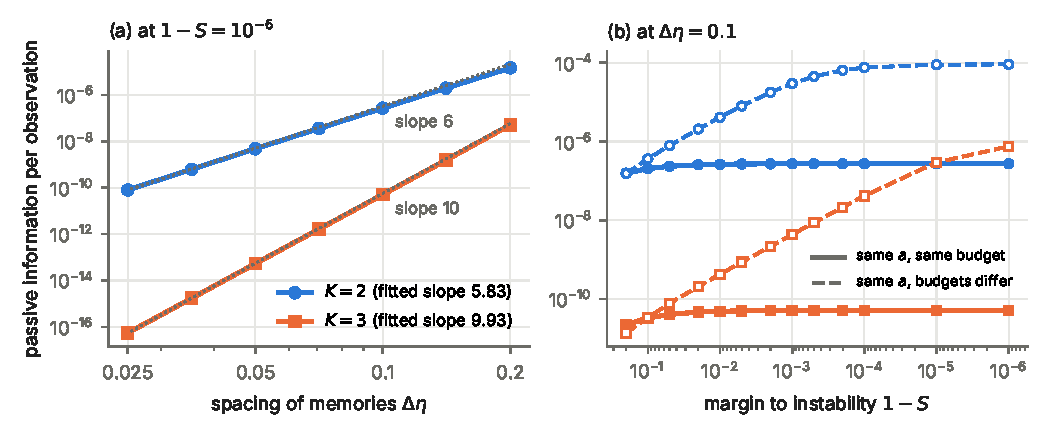
\includegraphics[width=\textwidth]{fig_barrier_admissible.pdf}
\caption{The passive barrier near instability. Both panels show the Gaussian Kullback--Leibler information per observation between the stationary price processes of two populations whose merged measures are the $K$-node Gauss and Gauss--Radau rules on memories spread over $\Delta\eta$ around $0.5$ (total weight $0.3$, impact $\kappa=0.5$). (a)~At a common persistence and a common feedback budget one millionth below instability, the information falls like $(\Delta\eta)^{4K-2}$ (dotted lines). (b)~With a common persistence and a common budget (solid; the Gauss--Radau weights rescaled by a factor $1+O((\Delta\eta)^{2K-1})$), the information stays bounded as the margin $1-S$ shrinks. With a common persistence and no rescaling (dashed), the budgets differ by order $(\Delta\eta)^{2K-1}$; the information then grows roughly like $(1-S)^{-1}$ until the margin reaches that gap, and levels off. Computed from the closed-form spectra.}
\label{fig:barrier}
\end{figure}


\section{Who needs composition, and what disclosure buys}\label{sec:supervision}

By Theorem~\ref{thm:eqinv}, composition is worth nothing to anyone trading on public information. It can still matter to a supervisor whose action is aimed at one group. This section gives a decision in which it does and the disclosure that removes the cost of learning it. It ends with a bound on what price-based targeting can achieve when a group can hide.

\paragraph{A decision in which attribution matters.} A supervisor must keep the feedback budget $S=a+\kappa\sum_iq_i$ below a prudential ceiling $\bar s$. It can either cut all activity uniformly or halt the largest verified class. The target is the feedback budget, not the spectral radius of the state matrix: in an already stable positive economy, imposing $S\le\bar s<1$ is a tighter prudential constraint, not a restoration of stability.


\begin{proposition}[Supervisory separation: market-wide versus targeted intervention]\label{prop:target}
Assume the positive stable model, known $a,\kappa$, and $a<\bar s<1$. Write $q_i=w_i/(1-r_i)$ and $R=S-\kappa\max_iq_i$ for the post-halt feedback budget.
\begin{enumerate}[label=(\roman*),itemsep=1pt]
\item A uniform scale $\theta$ meets the ceiling exactly when $a+\theta(S-a)\le\bar s$. Its largest feasible value is $\theta^*=\min\{1,(\bar s-a)/(S-a)\}$. The identity $S=1-\kappa/\sum_jh_j$ is algebraic; estimating this infinite sum requires a justified tail bound and an observation/noise model. It alone establishes no unconditional parametric learning rate.
\item For $K=2$, the Gauss and Gauss--Radau pair of Theorem~\ref{thm:kcohort} has limiting largest normalized weights $1/2$ and $3/4$. Thus $|S^G-S^R|=O((\Delta\eta)^3)$ and $q^R_{\max}-q^G_{\max}=W/(4(1-r_c))+O(\Delta\eta)$. For sufficiently small spacing, a nonempty interval of ceilings separates their post-halt decisions. For $N$ independent reset records with common Gaussian noise $\sigma^2 I$, both decision errors at most $1/4$ require
\[
 N\ge (2\Phi^{-1}(0.75)\sigma/\|h^G-h^R\|_2)^2
 \ge c\sigma^2(\Delta\eta)^{-6}.
\]
The record horizon and the response norm must be the same on both sides.
\item Tagged-flow estimation under Theorem~\ref{thm:discvalue}, a rate bound away from one, and a fixed nonzero decision margin gives a bounded sample requirement as the spacing shrinks. The target class must be mapped to an executable, verified class label; a largest latent atom alone supplies no such identity.
\end{enumerate}
\end{proposition}
The proof is in Supplement~\ref{app:decisionfull}. Proposition~\ref{prop:targetK} there extends part~(ii) to every $K$, with exponent $4K-2$.

\subsection{What class-tagged disclosure buys}


\begin{proposition}[Tagged flow removes the barrier]\label{prop:tagged}
Let the price $x_t$ be the causal stationary solution of the model driven by i.i.d.\ centred innovations of variance $\sigma_\xi^2\in(0,\infty)$ in a positive, stable economy, with stationary autocovariances $\gamma_x(s)=\sum_\ell c_\ell\lambda_\ell^{|s|}$ ($c_\ell\ge0$, $0\le\lambda_\ell<1$ the closed-loop modes). Suppose group $i$ has merged weight $w_i>0$ and the observer receives prices and each group's flow $\tilde u_{i,t}=u_{i,t}+\varepsilon_{i,t}$, $u_{i,t}=q_iy_{i,t}$, with i.i.d.\ centred measurement noise of finite variance $\sigma_f^2$, independent of the whole innovation sequence and hence of the whole price path. Then $\tilde u_{i,t}=r_i\tilde u_{i,t-1}+w_ix_t+e_{i,t}$ with $e_{i,t}=\varepsilon_{i,t}-r_i\varepsilon_{i,t-1}$, and the just-identified IV estimator of $\beta_i=(r_i,w_i)$ with instruments $Z_t=(x_{t-1},x_t)^\top$ satisfies $\sqrt T(\hat\beta_i-\beta_i)\to N(0,V_i)$,
\begin{equation}\label{eq:ivvar}
V_i=\Sigma_i^{-1}\Omega_i\Sigma_i^{-\top},\qquad \Sigma_i=\begin{pmatrix}w_iA_0&\gamma_x(1)\\ w_iA_1&\gamma_x(0)\end{pmatrix},\qquad \Omega_i=\sigma_f^2\bigl[(1+r_i^2)\Gamma_0-r_i(\Gamma_1+\Gamma_1^\top)\bigr],
\end{equation}
where $A_m=\sum_{s\ge0}r_i^s\gamma_x(s+m)$, $\Gamma_0=\begin{psmallmatrix}\gamma_x(0)&\gamma_x(1)\\ \gamma_x(1)&\gamma_x(0)\end{psmallmatrix}$ and $\Gamma_1=\E[Z_tZ_{t-1}^\top]$. The Jacobian determinant is
\begin{equation}\label{eq:ivdet}
\det\Sigma_i=w_i\sum_{\ell,m}c_\ell c_m\frac{1-\lambda_\ell\lambda_m}{1-r_i\lambda_m}\;>\;0 .
\end{equation}
$V_i$ depends only on group $i$'s own $(w_i,r_i)$, $\sigma_f^2$ and the price autocovariances. Two conclusions are distinct: (a) for each admissible economy, $\hat\beta_i$ has the stated limiting normal law; (b) on a uniformly stable family with stationary price variance at least $\gamma_{\min}>0$ and merged weights at least $w_{\min}>0$, the limiting covariance $V_i$ is bounded by a constant that does not depend on $|r_i-r_j|$. Statement (b) bounds the limit; it is not a central limit theorem that holds uniformly over the family.
\end{proposition}

\paragraph{Machine check.} Three pieces are machine-checked: the finite-sample reset-experiment version, with an error bound that does not depend on the spacing; the lower bound on the determinant of the population instrument matrix that does not depend on the spacing (\texttt{p1\_tagged\_iv\_determinant\_bound}); and the exact decomposition of the IV score into reporting-error terms with coefficients fixed by the price path plus two boundary terms (\texttt{p1\_iv\_boundary\_decomposition}). The stationary law of large numbers and the central limit theorem behind (a) are not machine-checked.


Each tagged flow follows $u_{i,t}=r_iu_{i,t-1}+w_ix_t$, a regression whose information about $w_i$ does not involve the other groups' rates; the closed form \eqref{eq:ivdet} matches the simulated Jacobian ($0.1330$ against $0.1322$ in a two-group economy with $4\times10^5$ periods). In simulation ($T=5{,}000$, 60 replications) the root-mean-square error of the recovered weights is flat in $\Delta\eta$ (fitted slope $0.011$, error between $5.8\times10^{-4}$ and $6.6\times10^{-4}$). This is the formal content of a disclosure regime such as a consolidated audit trail: tagging flow by participant class turns a polynomial barrier into an ordinary estimation problem.
Proposition~\ref{prop:tagged} says that tagging removes the barrier; the next result says by how much.

\begin{theorem}[Value of class-tagged disclosure]\label{thm:discvalue}
Take a rich class of Theorem~\ref{prop:esprit}: rates $r_c+\Delta\eta\,s$ with $s$ in a compact set of $\gamma$-separated ordered points that has nonempty interior and contains the Gauss and Gauss--Radau pair of Theorem~\ref{thm:kcohort}, and merged weights in a nondegenerate interval $[\omega_{\min},\omega_{\max}]$, $0<\omega_{\min}<\omega_{\max}$. In each reset experiment the observer applies a unit impulse and records the price response with independent $N(0,\sigma^2)$ noise per tap; under tagging it also records each class's flow response $f_{i,t}=w_i\sum_{s\le t}r_i^{\,t-s}h_s$ with independent $N(0,\sigma_f^2)$ noise per tap. Let $N_p$ and $N_t$ be the numbers of experiments needed, without and with tagging, for a fixed accuracy and confidence. There are constants $0<c\le C<\infty$, depending on $(\sigma,\sigma_f)$ and the class but not on $\Delta\eta$, such that
\begin{enumerate}[label=(\roman*),itemsep=1pt]
\item to recover the weights to a fixed accuracy smaller than half the weight difference between the Gauss and Gauss--Radau economies (so that recovering the weights decides between them), $c\le N_t\le C$, so $N_p/N_t\asymp(\Delta\eta)^{-(4K-2)}$;
\item to recover the rates to accuracy $c_0\Delta\eta$, for a fixed $c_0>0$ smaller than the radius of a ball contained in the class of rescaled nodes (so that no fixed guess meets the target), $c(\Delta\eta)^{-2}\le N_t\le C(\Delta\eta)^{-2}$, so $N_p/N_t\asymp(\Delta\eta)^{-(4K-4)}$.
\end{enumerate}
\end{theorem}

Proposition~\ref{prop:tagged} and Theorem~\ref{thm:discvalue} use different observation arrangements: the proposition concerns passive, stationary data with prices observed without noise, where the price is a valid instrument; the theorem concerns reset experiments with noisy prices. With noisy prices, regressing flow on the observed price is an errors-in-variables problem, which is why the theorem works from the known impulse instead.
\subsection{Partial disclosure}\label{sec:partial}

Actual regimes tag some traders and not others: Japan registers high-speed traders, India identifies algorithmic orders, and everyone else stays anonymous. Theorem~\ref{thm:discvalue} prices full tagging. The next result prices tagging some of the groups.

\begin{theorem}[Partial disclosure]\label{thm:partial}
In the reset experiments of Theorem~\ref{thm:discvalue}, let the flows of $m$ of the $K$ groups be recorded (tagged), and write $K'=K-m$ for the number of untagged groups.
\begin{enumerate}[label=(\roman*),itemsep=1pt]
\item \emph{Lower bound.} If $K'\ge2$, there are two $K$-group economies with rates in $r_c+\Delta\eta[-1,1]$ and positive weights, with identical tagged groups and with untagged groups forming the $K'$-node Gauss and Gauss--Radau pair of Theorem~\ref{thm:kcohort}, such that telling them apart from $N$ reset experiments, using the price records and the tagged flow records, with error probability below $1/4$ needs $N\ge c\,(\Delta\eta)^{-(4K'-2)}$.
\item \emph{Upper bound.} Let the tagged groups satisfy the conditions of Theorem~\ref{thm:discvalue}, and let the untagged groups range over a rich class of Theorem~\ref{prop:esprit} with $K'\ge2$ nodes. Estimate each tagged group from its flow records, subtract its contribution from the estimated kernel, and apply Prony's method with $K'$ nodes to the residual. This recovers the weights of all $K$ groups to any fixed accuracy from $N=C(\Delta\eta)^{-(4K'-2)}$ experiments.
\item \emph{One untagged group.} If $K'\le1$, the weights of all $K$ groups are recovered from a number of experiments that does not depend on $\Delta\eta$.
\end{enumerate}
The constants depend on $(\sigma,\sigma_f)$, the class and the tagged groups, not on $\Delta\eta$. So the cost of composition is that of the untagged groups alone: $N^*\asymp(\Delta\eta)^{-(4K'-2)}$ for $K'\ge2$.
\end{theorem}

\begin{proof}
(i) The two economies share the tagged groups, so their kernels differ only through the untagged pair, whose moments agree up to order $2K'-2$ (Theorem~\ref{thm:kcohort}); the kernel gap is therefore of order $(\Delta\eta)^{2K'-1}$ at every lag. The price impulse responses inherit this order through the closed-loop recursion, as in the proof of Theorem~\ref{thm:kcohort}, with constants that depend on the tagged groups only through the closed-loop stability margin. A tagged group's flow response, $f_{i,t}=w_i\sum_{s\le t}r_i^{\,t-s}h_s$, is the same linear map of the price response in both economies, so its mean difference is also of order $(\Delta\eta)^{2K'-1}$. With Gaussian noise the divergence of one experiment's full record is at most $C(\Delta\eta)^{4K'-2}$, and Le Cam's two-point lemma gives the bound.
(ii) As in the proof of Theorem~\ref{thm:discvalue}, the averaged price responses and least squares on each tagged class's flows estimate the tagged weights and rates with error $O_P(N^{-1/2})$, uniformly on the class and without dependence on $\Delta\eta$ or on the other groups. The kernel values $k_0,\ldots,k_{2K'-1}$ are smooth functions of the taps (proof of Theorem~\ref{prop:esprit}), so the residual kernel $k_j-\sum_{\rm tagged}\hat w_i\hat r_i^{\,j}$ estimates the untagged groups' kernel with error $O_P(N^{-1/2})$. Prony's method on these $2K'$ values is the estimator of Theorem~\ref{prop:esprit} with $K'$ nodes, whose error is the input error times order $(\Delta\eta)^{-(2K'-1)}$ (the rescaling of the centred moments). So the untagged weights have error $O_P(N^{-1/2}(\Delta\eta)^{-(2K'-1)})$, and $N=C(\Delta\eta)^{-(4K'-2)}$ suffices; the tagged weights are recovered at the faster rate.
(iii) With one untagged group of weight $v$ and rate $s$, $k_0=\sum_{\rm tagged}w_i+v$ and $k_1=\sum_{\rm tagged}w_ir_i+vs$, so $v$ and $s$ are smooth functions of $k_0$, $k_1$ and the tagged estimates, all estimated with error $O_P(N^{-1/2})$ independent of $\Delta\eta$. With none, this is Theorem~\ref{thm:discvalue}(i).
\end{proof}

\paragraph{Numerical check and machine check.} For $K=3$ with no tag and one tag, and $K=4$ with two tags, the exact divergence per experiment of the hard pair falls with $\Delta\eta$ at fitted slopes $10.05$, $6.02$ and $5.96$, against $10$, $6$ and $6$ (repository script \nolinkurl{reproduce.py}). Part~(i) is machine-checked on the joint records of prices and tagged flows, for records of any fixed length $T$ and a common noise variance $\sigma^2$ on prices and flows (with $\sigma_f\ne\sigma$, replace $\sigma$ by $\min(\sigma,\sigma_f)$): for any two economies that share their tagged groups and whose untagged node moments agree below order $n$, any test satisfies $4\sigma^2(1-\alpha_0-\beta_0)^2\le N(T+MT)\bigl(2W2^T(\Delta\eta)^nC_T(1+W_tT)\bigr)^2$ (\texttt{p1\_partial\_lower\_bound\_matched}, \nolinkurl{Paper1PartialDisclosureLower.lean}); with the matched $K'$-node pair of Theorem~\ref{thm:kcohort}, $n=2K'-1$. The algebraic steps of (ii) and (iii) are machine-checked too (\nolinkurl{Paper1PartialDisclosure.lean}), and so is the deterministic core of (ii): if the kernel taps are estimated within $e_k$ and the tagged weights and rates within $e_w$ and $e_r$, an ordered $K'$-node representation matching the residual moments exists, is unique and recovers every untagged weight within $L\,2^{2K'}\eta(\Delta\eta)^{-(2K'-1)}$, with $\eta=e_k+m(e_w+W_t\,2K'\,e_r)$ (\texttt{p1\_partial\_upper\_deterministic}, \nolinkurl{Paper1PartialDisclosureUpper.lean}). The $O_P(N^{-1/2})$ rates of the inputs are on paper, and the whole estimator is checked by Monte Carlo: subtract-then-Prony gives weight errors growing like $(\Delta\eta)^{-(2K'-1)}$, fitted slopes $-5.07$, $-3.02$ and $0.36$ for $K'=3,2,1$ untagged groups of three, against $-5$, $-3$ and $0$ (repository script \nolinkurl{reproduce.py}).

\subsection{Traders who respond to being watched}\label{sec:hiding}

The results so far take the groups' rules as given. A group that expects a targeted action has a reason to change its rule. Sufficiency bounds what a supervisor who relies on prices can then achieve.

\begin{proposition}[Hiding caps targeting]\label{prop:hiding}
A supervisor observes prices, under any probes and for a record of any length, and then targets a given group or not. Being targeted costs the group $P>0$. The group chooses among available rules. Rule $\rho$ has a private cost $C(\rho)\ge0$ and leads to targeting with probability $\pi(\rho)$. Suppose one available rule $\rho_0$, with cost $C_0$, gives the population the kernel of a population that the supervisor targets with probability $\alpha$.
\begin{enumerate}[label=(\roman*),itemsep=1pt]
\item $\pi(\rho_0)=\alpha$, whatever the supervisor's probes, record length and decision rule.
\item Every rule $\rho^*$ that minimizes the group's expected cost $C(\rho)+P\pi(\rho)$ satisfies
\[
\pi(\rho^*)\ \le\ \alpha+\frac{C_0-C(\rho^*)}{P}\ \le\ \alpha+\frac{C_0}{P}.
\]
\item Suppose the group has two rules: its original rule, with cost zero and targeting probability $\pi_T$ on a record of length $T$, and $\rho_0$. It adopts $\rho_0$ whenever $\pi_T>\alpha+C_0/P$. If $\pi_T\to1$ and $P(1-\alpha)>C_0$, this holds for all large $T$, and the targeting probability is then $\alpha$.
\end{enumerate}
\end{proposition}

\begin{proof}
(i) By Theorem~\ref{thm:eqinv}, populations with the same kernel give the same law of the price record for every probe sequence and every insider and dealer rule. The supervisor's decision is a function of that record and of its own randomization. (ii) $C(\rho^*)+P\pi(\rho^*)\le C_0+P\alpha$ by optimality, and $C(\rho^*)\ge0$. (iii) The original rule costs $P\pi_T$ and $\rho_0$ costs $C_0+P\alpha$.
\end{proof}


\section{Scope and limits}\label{sec:scope}

\paragraph{Linearity.} Sufficiency (Theorem~\ref{thm:eqinv}, Proposition~\ref{prop:anylinear}) needs aggregate feedback flow to be a linear function of past public signals, plus independent idiosyncratic shocks if there are any. With group-specific Gaussian demand shocks, a second aggregate enters, the spectral density of the aggregate shock process, and the equivalence class shrinks accordingly (Supplement~\ref{app:eqinv}). The passive results of Section~\ref{sec:cost} are stated for Gaussian innovations, the least favourable case: for any news law whose location divergence is quadratically bounded the passive orders are unchanged and the constant improves by the factor $\sigma^2I^*_f\ge1$ (\citealp[Proposition~S16.2]{niroula2026full}). Laws outside that class, such as news with bounded support, are not analysed. Saturating rules are treated in \citet[Section~S6]{niroula2026full}. Other nonlinear rules, and traders who change their rules as they learn, are outside the theorems. \citet{niroula2026a} report simulations of stylized nonlinear rules and of online learners trained in the closed loop. In those simulations, the costs of Section~\ref{sec:cost} hold when the competing populations' feedback weights match. Populations whose learned weights differ are told apart by those weights instead. Hard thresholds hide groups from small probes altogether. These are simulations, not theorems.

\paragraph{Exponential memory.} The identification and cost results need memory to be a finite mixture of exponentials. For general completely monotone memory, \citet{niroula2026a} prove that the minimax accuracy for the memory distribution is of exact order $1/\log(N/\sigma^2)$. This is the severe ill-posedness of inverting a Laplace transform \citep{epstein2008}. Halving the error then squares the data needed, instead of multiplying it by a constant.

\paragraph{The observer.} The lower bounds hold for an observer who knows $(a,\kappa)$ and the noise law, so they hold a fortiori without that knowledge. The upper bound of Theorem~\ref{prop:esprit} also holds in one running market from an unknown state, with random-sign probes and news of any law with finite variance (\citealp[Theorem~S16.1]{niroula2026full}); the other upper bounds are stated for reset experiments. Strategic responses to being observed are modelled in Proposition~\ref{prop:hiding} and Supplement Section~\ref{app:dynamic} (traders who learn from prices, and a game of surveillance and hiding). Everywhere else the groups do not change their rules when probed.

\paragraph{Evidence.} \citet{niroula2026a} report pre-specified tests on two sets of trader-class reports: the CFTC's weekly Commitments of Traders in twenty futures markets and Binance's class ratios in 30 perpetual markets. Of 23 recorded outcomes, 11 pass. None is a direct test of a result in this paper: all use class positions or account ratios rather than executed flow tagged by class. The class reports constrain the persistence of class positions far more tightly than prices do. They do not identify learning memory, because that persistence can also reflect turnover, reporting aggregation or inventory retention. A pre-registered out-of-sample test of the feedback premise on Taiwan's tagged exchange flows (spec P1T, holdout 2019--2023; \citet{niroula2026a} report every diagnostic) gives the following. $D=0.0426$ $[0.0206, 0.0643]$, $p=0.000$, meets the registered supportive criterion. The pre-specified reverse-causality check gives $D=-0.0065$ $[-0.0316, 0.0165]$, which does not meet it. Under the registered rule that check is inconclusive rather than contrary: its interval contains both zero and the smallest effect of interest, and 68\% of stocks keep a positive gain after the adjustment (median $0.012$). By calendar year the primary gain meets the criterion in 2019--2021 and not in 2022--2023. The registered verdict is `supportive'. Read with its pre-specified diagnostic, the test does not provide evidence of feedback beyond prices revealing past flow. We do not claim that tagged flow in Taiwan responds to price deviations. The registered test is supportive, but its pre-specified diagnostic attributes the gain to reverse causality.

A second test, of the two-layer prediction of \citet[Section~S6]{niroula2026full}, is registered on Binance perpetual futures (spec P7S, amendment A1). Its primary sample is retrospective (July 2024 to October 2026), specified in November 2026 after the sample period, and a prospective window from November 2026 serves as a replication. The primary test was run once on 11 November 2026. A pre-specified test on Binance perpetual futures was inconclusive (calm difference $-0.002$, 90\% interval $[-0.007, 0.004]$; difference-in-differences $0.041$, $p=0.553$). It neither supports nor contradicts the prediction of \citet[Section~S6]{niroula2026full}. A prospective replication protocol on Binance perpetual futures is pre-specified with fixed development thresholds (August to October 2026) serving as an externally locked template for subsequent window observation.

\paragraph{Open problems.} The companion paper \citep{niroula2026c} answers several further questions: a long-lived insider cannot reveal or manipulate the groups' memory in a stable market, and a rational market maker nets feedback out (Companion Proposition~\ref{prop:insider}); a cascade after a breach has an exact threshold under mechanical impact (Companion Theorem~\ref{thm:cascade}); dead-band traders are identifiable by large probes (Companion Proposition~\ref{prop:deadband}). It also gives forward-looking dealers (several equilibria above the threshold; Companion Proposition~\ref{prop:reecascade}), saturation of every order (Companion Proposition~\ref{prop:smoothn}), a parametric rate for noisy stress identification with smooth shapes (Companion Proposition~\ref{prop:stressrate}) and the information content of learning traders (Companion Proposition~\ref{prop:learners}). It also covers a group that chooses its rule against an insider (Companion Proposition~\ref{prop:insidergame}), the path of a cascade, including slow-moving capital (Companion Proposition~\ref{prop:cascadedyn}), a parametric rate under hard limits (Companion Proposition~\ref{prop:hardrate}), the cost of composition when traders are nonlinear (Companion Proposition~\ref{prop:nlcost}), and the largest-weight comparison for every $K$ (Proposition~\ref{prop:maxweight}). What remains open: uniqueness of the insider game in cases where residual monotonicity fails (\citealp[Proposition~S17.3]{niroula2026full}); cascades whose dealers face richer constraints than a constant holding cost; hard-limit configurations whose kinks coincide; and upper bounds for nonlinear traders who share a leverage.



\section{Proofs of the main results}\label{app:proofs}

\paragraph{A lemma used in the proofs.}
\begin{lemma}[Positive price-response geometry]\label{lem:cm}
In the positive, stable economy the impulse response is a nonnegative mixture of decaying exponentials,
\[
h_j=\sum_\ell \omega_\ell\lambda_\ell^j,\qquad \omega_\ell\ge0,\quad \sum_\ell\omega_\ell=\kappa,\quad 0\le\lambda_\ell<1 .
\]
It is completely monotone and nonincreasing; its peak is the direct impact $\kappa$, even though $J$ is non-normal. In price/memory coordinates the price-only gain is $\sup_t\|e_x^\top J^t\|_2=1$.
\end{lemma}

\paragraph{Lemma~\ref{lem:cm}.} Omit zero-weight groups. For $a>0$ put $b_i=\kappa q_i$ and
\[
T={\rm diag}\bigl(\sqrt a,\sqrt{b_1/\eta_1},\ldots\bigr),\qquad u=\bigl(\sqrt a,\sqrt{b_1\eta_1},\ldots\bigr)^\top .
\]
The price-first transition becomes the symmetric matrix $J'=TJT^{-1}={\rm diag}(0,r_1,\ldots)+uu^\top$, the input transforms to $\kappa u$ and $J'e_x=\sqrt a\,u$, so $h_j=(\kappa/a)e_x^\top(J')^{j+1}e_x$. The spectral decomposition of $J'$ gives nonnegative weights summing to $h_0=\kappa$, and Schur stability puts the eigenvalues in $[0,1)$. The case $a=0$ follows by continuity. A nonnegative mixture of decaying geometric sequences is completely monotone. Since $J$ is nonnegative with row sums at most one, every price row of $J^t$ has $\ell_1$, hence $\ell_2$, norm at most one, attained at $t=0$.


\paragraph{Lemma~\ref{lem:micro}.} (i) For $v_{t+1}=v_t+\zeta_{t+1}$ and $r_t=v_t+\nu_t$, the steady-state prior variance $P$ solves $P=P\sigma_\nu^2/(P+\sigma_\nu^2)+\sigma_\zeta^2$, i.e.\ $P^2-\sigma_\zeta^2P-\sigma_\zeta^2\sigma_\nu^2=0$, whose positive root is $P=\bigl(\sigma_\zeta^2+\sqrt{\sigma_\zeta^4+4\sigma_\zeta^2\sigma_\nu^2}\bigr)/2$. The gain is $\eta=P/(P+\sigma_\nu^2)\in(0,1)$, which simplifies to \eqref{eq:kgain}, and the update $\hat v_{t+1}=\hat v_t+\eta(r_t-\hat v_t)$ has the stated form. (ii) $\nabla_\theta\tfrac12H(x_t-\theta)^2=-H(x_t-\theta)$, so $\theta_{t+1}=(1-\gamma)\theta_t+\alpha H(x_t-\theta_t)=(1-\eta)\theta_t+\eta qx_t$ with $\eta=\gamma+\alpha H$ and $q=\alpha H/\eta$.


\paragraph{Theorem~\ref{thm:merged}.} With zero initial states, $y_{i,t}=\sum_{s\le t}\eta_ir_i^{t-s}x_s$, so $\sum_iq_iy_{i,t}=\sum_{s\le t}k_{t-s}x_s$ and every response is determined by $(a,\kappa,k)$, hence by $M$. Conversely, equal responses for all probes imply equal $H$, hence equal $G$, and partial fractions of $G$ identify the distinct poles with nonzero residues $w_i$, i.e.\ $M$. After cancellation, $H=\kappa zD(z)/[(z-a)D(z)-\kappa N(z)]$ with $D=\prod(z-r_i)$ and $N(z)=\sum_iw_iz\prod_{j\ne i}(z-r_j)$, as in \eqref{eq:H}; at a retained $r_i$ the denominator equals $-\kappa N(r_i)=-\kappa w_ir_i\prod_{j\ne i}(r_i-r_j)\neq0$ (memory rates are positive because $\eta_i<1$), so no root of $D$ cancels. The numerator $\kappa zD(z)$ has no roots other than $0$ and the $r_i$, so these are the only possible cancellations. The remaining numerator factor $z$ cancels if and only if the denominator vanishes at $0$; since $N(0)=0$ the denominator there equals $-aD(0)$, which is nonzero for $a>0$ and zero for $a=0$. Hence the McMillan degree, which is the dimension of a minimal realization, is $1+|{\rm supp}(M)\cap(0,1)|$ for $a'\neq0$ and $|{\rm supp}(M)\cap(0,1)|$ for $a'=0$ (an atom at rate $0$, a group with $\eta=1$, contributes the constant $M(\{0\})$ to $G$ and no pole, so it shifts $a$ to $a'=a+\kappa M(\{0\})$ and the argument above applies with $a'$) (numerically, the rank of the Hankel matrix of $(h_j)_{j\ge1}$ is $K+1$ and $K$ respectively for $K=1,2,3$). For (ii), direct algebra gives
\[
G_\delta(z)-G_0(z)=-\frac{qz(z-1)\delta^2}{(z-1+\bar\eta)\bigl((z-1+\bar\eta)^2-\delta^2\bigr)} .
\]
The denominator is the product of the three linear factors $z-r$ with $r\in\{1-\bar\eta,\,1-\bar\eta\pm\delta\}$, all in $[\epsilon,1-\epsilon]$ by assumption; on $|z|=1$ each satisfies $|z-r|\ge1-r\ge\epsilon$, so $|G_\delta-G_0|\le2q\delta^2/\epsilon^3$ there. Uniform stability gives $M_H=\sup|H_\theta|<\infty$, and the identity $H_\delta-H_0=z^{-1}H_\delta H_0(G_\delta-G_0)$, whose factor $z^{-1}$ has modulus one on the circle, gives an $\ell_2$ gain at most $C_{\mathcal F}\delta^2$. The mean difference of a power-constrained probe has squared norm at most $C_{\mathcal F}^2\delta^4PT$; the equal-noise KL is at most $C_{\mathcal F}^2\delta^4PT/(2\sigma_\nu^2)$, and Pinsker's inequality with total variation at least $1-2\alpha$ gives \eqref{eq:Tpower}.


\paragraph{Theorem~\ref{thm:kcohort}.} Let $(s^A,\omega^A)$ and $(s^B,\omega^B)$ be the $K$-point Gauss and Gauss--Radau rules for the uniform weight on $[-1,1]$, normalized to unit mass. Both are positive and exact for polynomials of degree $2K-2$, and their moments of degree $2K-1$ differ by $g_K\neq0$. To see that $g_K\ne0$, let the Radau nodes be $-1,s_2,\ldots,s_K$ and put $P(s)=(s+1)\prod_{j\ge2}(s-s_j)^2$. This is monic of degree $2K-1$ and vanishes at every Radau node, so the Radau rule gives it $0$. Gauss is exact to degree $2K-1$, so it gives $\int P\,d\mu>0$, since $P\ge0$ on $[-1,1]$ and vanishes only at the nodes. The two rules agree on every lower-degree term, so they differ on $s^{2K-1}$. Put $r=r_c+\Delta\eta\,s$ and weights $W\omega$, and let $\mu^X_j=W\sum_i\omega^X_i(s^X_i)^j$ for $X\in\{A,B\}$. Then $|\mu^X_j|\le W$, and $\mu^A_j=\mu^B_j$ for $j\le2K-2$.

\emph{Kernel gap.} By the binomial theorem, $k^X_m=\sum_j\binom mj r_c^{m-j}(\Delta\eta)^j\mu^X_j$. So, with $n=2K-1$, $\Delta k_m=k^A_m-k^B_m=\sum_{j\ge n}\binom mj r_c^{m-j}(\Delta\eta)^j(\mu^A_j-\mu^B_j)$. Since $\binom mj\le\binom mn\binom{m-n}{j-n}$ for $j\ge n$, this gives $|\Delta k_m|\le2W\binom mn(\Delta\eta)^n(r_c+\Delta\eta)^{m-n}$. Summing with $\sum_m\binom mn x^{m-n}=(1-x)^{-(n+1)}$ gives $\|\Delta k\|_1\le2W(\Delta\eta)^{2K-1}/(1-r_c-\Delta\eta)^{2K}$ over all lags.

\emph{Response gap.} Let $\varsigma=a+\kappa W/(1-r_c-\Delta\eta)<1$, the theorem's hypothesis. Each kernel has $\|k^X\|_1\le W/(1-r_c-\Delta\eta)$. From $h_0=\kappa$ and $h_{t+1}=ah_t+\kappa\sum_jk_jh_{t-j}$, every partial sum of $|h^B|$ is at most $\kappa/(1-\varsigma)$. The difference $\Delta h=h^A-h^B$ has $\Delta h_0=0$ and $\Delta h_{t+1}=a\Delta h_t+\kappa\sum_j\bigl(k^A_j\Delta h_{t-j}+\Delta k_jh^B_{t-j}\bigr)$, so every partial sum of $|\Delta h|$ is at most $\kappa\|\Delta k\|_1\|h^B\|_1/(1-\varsigma)$. Hence, for every horizon,
\[
\|h^A-h^B\|_2\le\|h^A-h^B\|_1\le C_U(\Delta\eta)^{2K-1},\qquad C_U=\frac{2\kappa^2W}{(1-r_c-\Delta\eta)^{2K}(1-\varsigma)^2}.
\]
In the other direction, $\Delta k_j=0$ for $j<2K-1$, so by induction $\Delta h_t=0$ for $t\le2K-1$, and $\Delta h_{2K}=\kappa\,\Delta k_{2K-1}h^B_0=\kappa^2Wg_K(\Delta\eta)^{2K-1}$. When the taps $h_0,\ldots,h_{T-1}$ are observed with $T\ge2K+1$, this gives $\|h^A-h^B\|_2\ge\kappa^2W|g_K|(\Delta\eta)^{2K-1}$. With $T\le2K$ the observed responses coincide. The impossibility bound holds for every $T$, since it uses only the upper order.

\emph{Testing.} $N$ reset experiments have divergence $N\|h^A-h^B\|_2^2/(2\sigma^2)$. By Pinsker's inequality, a test whose two error probabilities are at most $\alpha$ needs divergence at least $2(1-2\alpha)^2$. So $N\ge4(1-2\alpha)^2\sigma^2(\Delta\eta)^{-(4K-2)}/C_U^2$, and the constant does not depend on $T$. For the $W_1$ version, the two merged measures are the images of the fixed normalized rules under $s\mapsto r_c+\Delta\eta\,s$ scaled to mass $W$, so their distance is $W\Delta\eta$ times the distance $2c_K>0$ between the rules, and the same two-point argument applies with the metric loss.


\paragraph{Theorem~\ref{prop:passive}.} For stationary Gaussian processes with spectral densities $f_j\propto|H_j(e^{i\omega})|^2$, the divergence rate is
\[
D=\frac1{4\pi}\int_{-\pi}^{\pi}\bigl(\varrho-1-\log\varrho\bigr)\,d\omega,\qquad \varrho=f_1/f_0=|H_1/H_0|^2 .
\] By the resolvent identity, $H_1/H_0-1=z^{-1}H_1\Delta G$ with $\Delta G=G_1-G_0$, and uniform stability bounds $|H_1|$ on the circle, so $u\equiv\varrho-1=2\,{\rm Re}(z^{-1}H_1\Delta G)+O(|\Delta G|^2)$. Write $G(z)=\sum_kw_k\phi(z,\eta_k)$, with $w_k$ the group weights (any factor of $\eta_k$ is absorbed in $\phi$), where $\phi$ is analytic in $\eta$ on a neighbourhood of $[\eta_{\min},\eta_{\max}]$ uniformly for $|z|=1$ (its pole $z=1-\eta$ stays inside the disk). Expanding $\phi$ around $\bar\eta$, $\Delta G=\sum_{j\ge0}\frac{\partial_\eta^j\phi(z,\bar\eta)}{j!}\,\Delta\tilde M_j$, where $\tilde M_j=\sum_kw_k(\eta_k-\bar\eta)^j$. For the pair, $\Delta\tilde M_0=\Delta\tilde M_1=0$ and $\Delta\tilde M_2=q\delta^2$; for the moment-matched economies, $\Delta\tilde M_j=0$ for $j\le2$ and $\Delta\tilde M_3=4\tau p_-p_+(\Delta\eta)^3$ by (22) of \citet{niroula2026full}; for the $K$-group Gauss and Gauss--Radau economies with rates $\bar\eta+\Delta\eta\,s$ and weights $W\omega$, both rules integrate polynomials of degree $2K-2$ exactly, so $\Delta\tilde M_j=W(\Delta\eta)^j\sum_k(\omega^A_k(s^A_k)^j-\omega^B_k(s^B_k)^j)$ vanishes for $j\le2K-2$ and equals $\pm Wg_K(\Delta\eta)^{2K-1}\neq0$ at $j=2K-1$. Higher terms are smaller by a factor of the spacing: $|\Delta\tilde M_j|\le2W(\Delta\eta)^j$, and analyticity of $\phi$ in $\eta$ on a disk of radius $\varrho>0$ around $\bar\eta$, uniformly on the circle, gives $|\partial_\eta^j\phi|/j!\le C\varrho^{-j}$, so for $\Delta\eta<\varrho/2$ the tail beyond the first nonzero term is $O((\Delta\eta)^{j_0+1})$. Hence $\sup_\omega|u|=O(\delta^2)$, $O(\tau(\Delta\eta)^3)$, respectively $O((\Delta\eta)^{2K-1})$, and $u=c(\omega)\epsilon+o(\epsilon)$ with $\epsilon=\delta^2$, $\tau(\Delta\eta)^3$ or $(\Delta\eta)^{2K-1}$ and $c(\omega)$ proportional to $2\,{\rm Re}\bigl(z^{-1}H_0\,\partial^{j_0}_\eta\phi(\cdot,\bar\eta)\bigr)/j_0!$, $j_0=2$, $3$ or $2K-1$. The function $c$ does not vanish identically: $f=z^{-1}H_0\partial^j_\eta\phi$ is analytic outside the disk including at infinity, where it vanishes, and is not identically zero; an analytic function on the exterior whose real part vanishes on the circle is an imaginary constant, which here would have to be zero. For $|u|\le\frac12$, $u^2/4\le u-\log(1+u)\le u^2$, so $D\asymp\int c(\omega)^2d\omega\,\epsilon^2$, which gives (i)--(iii). The sample requirements need a finite-$T$ bound that is uniform in the separation, which we obtain directly. The first $T$ observations are $N(0,\Sigma_j)$ with $\Sigma_j$ the $T\times T$ Toeplitz matrices of the spectral densities $f_j=\sigma^2|H_j(e^{i\omega})|^2$. On the compact, uniformly stable family the transfer functions have no zeros or poles on the circle (Theorem~\ref{thm:minphase}), so $0<\underline f\le f_j\le\bar f<\infty$ with constants that do not depend on the separation. A Toeplitz matrix has eigenvalues within the range of its symbol, so $\lambda_{\min}(\Sigma_0)\ge\underline f$ and $\|\Sigma_1-\Sigma_0\|\le\sup_\omega|f_1-f_0|=\sup_\omega f_0|u|\le\bar f\sup_\omega|u|$. With $A=\Sigma_0^{-1/2}\Sigma_1\Sigma_0^{-1/2}$, whose eigenvalues lie in $[\underline f/\bar f,\bar f/\underline f]$, the inequality $\lambda-1-\log\lambda\le(\lambda-1)^2/\lambda$ gives
\[
\KL(P_1^T\|P_0^T)=\tfrac12\sum_k(\lambda_k-1-\log\lambda_k)\le\frac{\bar f}{2\underline f}\,\|A-I\|_F^2\le\frac{\bar f}{2\underline f}\,T\Bigl(\frac{\bar f}{\underline f}\Bigr)^2\sup_\omega|u|^2\le C\,T\epsilon^2,
\]
with $C$ independent of $T$ and of the separation, because $\sup_\omega|u|=O(\epsilon)$ uniformly. The Bretagnolle--Huber inequality \citep[Lemma 2.6]{tsybakov2009} then gives the stated lower bounds on $T$ for every $T$, not only asymptotically. For a fixed pair, $T^{-1}\KL(P_1^T\|P_0^T)\to D$ and Stein's lemma (one error fixed) and the Chernoff bound (both errors vanishing) give the error exponents of the likelihood-ratio test, of the same order in the separation; that statement is pointwise in the pair.


\paragraph{Theorem~\ref{thm:minphase}.} In the delay variable $\lambda=z^{-1}$, $H=\kappa\prod_i(1-r_i\lambda)/\bigl[(1-a\lambda)\prod_i(1-r_i\lambda)-\kappa\lambda\sum_iw_i\prod_{j\ne i}(1-r_j\lambda)\bigr]$, which is \eqref{eq:H} divided through by $z^{K+1}$; its nonstructural zeros are the memory rates, which do not cancel under the nondegenerate assumptions of Theorem~\ref{thm:minphase}. In the z-plane there is also the structural timing zero at zero: the numerator is proportional to $z\prod_i(z-r_i)$. Stability puts the poles inside the disk. A rational spectral density $\sigma^2|H(e^{i\omega})|^2$ has a unique minimum-phase factor up to a unimodular constant, which is $H$; Theorem~\ref{thm:merged} then gives the merged measure.


\paragraph{Proposition~\ref{prop:tagged}.} With tagged flow, $u_{i,t}=r_iu_{i,t-1}+w_ix_t$ holds exactly and involves only group $i$, so $\tilde u_{i,t}=r_i\tilde u_{i,t-1}+w_ix_t+e_{i,t}$ with the MA(1) error $e_{i,t}$. Prices are independent of the measurement noise, so $\E[Z_te_{i,t}]=0$ and, by the ergodic theorem for the stationary linear price process, the IV estimator is consistent when $\Sigma_i=\E[Z_t(\tilde u_{i,t-1},x_t)]$ is nonsingular. Since $u_{i,t-1}=w_i\sum_{s\ge0}r_i^sx_{t-1-s}$, $\E[x_{t-1}u_{i,t-1}]=w_iA_0$ and $\E[x_tu_{i,t-1}]=w_iA_1$, which gives $\Sigma_i$. The price is a nonnegative mixture of geometric responses to its innovation (Lemma~\ref{lem:cm}), so $\gamma_x(s)=\sum_\ell c_\ell\lambda_\ell^{s}$ with $c_\ell=\sigma_\xi^2\kappa^{-2}\omega_\ell\sum_m\omega_m/(1-\lambda_\ell\lambda_m)\ge0$; substituting, $\det\Sigma_i=w_i(\gamma_x(0)A_0-\gamma_x(1)A_1)=w_i\sum_{\ell,m}c_\ell c_m(1-\lambda_\ell\lambda_m)/(1-r_i\lambda_m)$, each term positive. By summation by parts, $\sum_{t=1}^TZ_te_{i,t}=\sum_{t=1}^T(Z_t-r_iZ_{t+1})\varepsilon_{i,t}+O_P(1)$. Since $(\varepsilon_{i,t})$ is i.i.d.\ with mean zero and variance $\sigma_f^2$ and independent of the whole stationary price process, the summands $m_t=(Z_t-r_iZ_{t+1})\varepsilon_{i,t}$ form a stationary ergodic martingale difference sequence with respect to $\mathcal F_t=\sigma((x_s)_{s\in\mathbb Z},\varepsilon_{i,s}:s\le t)$, with $\E[m_tm_t^\top]=\sigma_f^2[(1+r_i^2)\Gamma_0-r_i(\Gamma_1+\Gamma_1^\top)]=\Omega_i$, so the Billingsley--Ibragimov martingale central limit theorem gives \eqref{eq:ivvar}. On a uniformly stable family the modes and weights lie in a compact set with $\lambda_\ell\le\bar\lambda<1$, so with $w_i\ge w_{\min}>0$ we get $\det\Sigma_i\ge w_{\min}(1-\bar\lambda^2)\gamma_x(0)^2>0$ and $\|\Omega_i\|$ is bounded, uniformly in the spacing.


\paragraph{Theorem~\ref{prop:esprit}.}
\begin{proof}
The kernel values $k_m=\sum_iw_ir_i^m$ are the power moments of the merged measure. The closed-loop recursion $h_t=ah_{t-1}+\kappa\sum_mk_mh_{t-1-m}$ (plus $\kappa$ at $t=0$) can be solved for $k_0,\ldots,k_{2K-1}$ from $h_1,\ldots,h_{2K}$. Because $h_0=\kappa$ is a known primitive, each $k_m$ is a polynomial in $h_1,\ldots,h_{m+1}$ with coefficients depending on $(a,\kappa)$ (the only division is by $\kappa h_0=\kappa^2$), so on the bounded set of responses within sup-distance $1$ of the class this map is $L_h$-Lipschitz, with $L_h$ depending on the class but not on $\Delta\eta$. Let $E$ be the event $\max_{1\le t\le2K}|\bar h_t-h_t|\le\sigma N^{-1/2}\sqrt{2\log(4K/\beta)}$, where $\bar h_t$ averages the $N$ responses; a Gaussian tail bound and a union bound over the $2K$ estimated taps give $P(E)\ge1-\beta$. On $E$, and provided this radius is at most $1$, the estimated kernel values satisfy $\max_m|\hat k_m-k_m|\le L_h\sigma N^{-1/2}\sqrt{2\log(4K/\beta)}$. Centring at $r_c$ is a fixed triangular linear map, $\mu_m=\sum_{j\le m}\binom mj(-r_c)^{m-j}k_j$, and $\mu_m=(\Delta\eta)^m t_m$ with $t_m=\sum_iw_is_i^m$. The map $F:(s,\omega)\mapsto(t_0,\ldots,t_{2K-1})$ does not depend on $\Delta\eta$; its Jacobian is a confluent Vandermonde matrix with determinant $\prod_i\omega_i\prod_{i<j}(s_i-s_j)^4$, bounded away from zero on the compact class. On ordered, $\gamma$-separated nodes $F$ is injective, because a measure with $K$ distinct atoms is determined by its first $2K$ moments. A $C^1$ map that is injective on a compact set $Q$ and has a nonsingular Jacobian there is injective on an open neighbourhood $U$ of $Q$: otherwise there are $x_n\ne y_n$ with $F(x_n)=F(y_n)$ and distance to $Q$ tending to zero, whose limits $x,y\in Q$ satisfy $F(x)=F(y)$, so $x=y$, contradicting local injectivity at $x$. Applying the quantitative inverse function theorem uniformly on $Q$, there are $\rho_0>0$ and $L<\infty$, uniform over the class, such that $F(U)$ contains the ball of radius $\rho_0$ around every point of $F(Q)$ and the single inverse $F^{-1}:F(U)\to U$ is $L$-Lipschitz on each such ball. An error $e$ in $\mu_m$ is an error $e(\Delta\eta)^{-m}$ in $t_m$, largest at $m=2K-1$. Since $\Delta\eta<1$ and the centring map is fixed, on $E$ we get $\|\hat t-t\|_\infty\le C_1\sqrt{\log(4K/\beta)}\,\epsilon_N$ with $C_1$ equal to $\sqrt2L_h$ times the norm of the centring map; and because $\sigma N^{-1/2}\sqrt{2\log(4K/\beta)}\le\sqrt2\,\epsilon_N\sqrt{\log(4K/\beta)}$, the radius condition holds whenever $c_0\le1/\sqrt2$. When this is below $\rho_0$, $\hat t$ lies in the ball where $F^{-1}$ is $L$-Lipschitz. For an input in such a ball, $x=F^{-1}(\hat t)$ has $K$ distinct nodes and nonzero weights, so the $K\times K$ Hankel matrix of $\hat t$ is nonsingular and Prony's method returns exactly $x$: the Prony polynomial is determined uniquely by the Hankel system, and since the $K$ real nodes of $x$ reproduce $\hat t$ it equals $\prod_i(z-\hat s_i)$, so its roots are real and distinct and no complex pair can appear; Prony's method computes the algebraic inverse of the moment map up to the order of the atoms, so, listing its output in increasing order of rate (which the error bound below keeps unambiguous once $C\sqrt{\log(4K/\beta)}\,\epsilon_N<\gamma/2$), its output is $F^{-1}(\hat t)$ and the stated bound follows with $C=LC_1$ and $c_0=\min\{\min(\rho_0,\gamma/(2L))/C_1,\,1/\sqrt2\}$, which also keeps $C\sqrt{\log(4K/\beta)}\,\epsilon_N<\gamma/2$. No separate root-perturbation bound is needed: on the ball where $F^{-1}$ is $L$-Lipschitz, Prony's roots and weights are the coordinates of $F^{-1}(\hat t)$, so the conditioning of the root step is part of $L$ (for an explicit step-by-step analysis of Prony's method with clustered exponents see \citealp{katz2023}). The matching statement requires the class to contain the Gauss and Gauss--Radau pair of Theorem~\ref{thm:kcohort} (ordered nodes with separation at least the smaller of their two minimum gaps, and weights within $[\omega_{\min},\omega_{\max}]$ after scaling to total weight $W$); for any such class the orders match, with constants that depend on the class.
\end{proof}
\paragraph{Theorem~\ref{thm:discvalue}.}
\begin{proof}
$N_p\asymp\sigma^2(\Delta\eta)^{-(4K-2)}$ by Theorems~\ref{thm:kcohort} and~\ref{prop:esprit}. \emph{Upper bounds.} Average the $N$ price responses to estimate $h$ with error of order $\sigma N^{-1/2}$ per tap. Given $h$, class $i$'s mean flow is a two-parameter family $F(w_i,r_i;h)$ whose Jacobian columns $\sum_sr_i^{t-s}h_s$ and $w_i\sum_s(t-s)r_i^{t-s-1}h_s$ are linearly independent, with a Gram determinant bounded below uniformly on the class because $w_i\ge\omega_{\min}$, the rates lie in a compact subset of $(0,1)$ and $h_0=\kappa>0$; the bound does not involve the other classes or $\Delta\eta$. Least squares on class $i$'s flows with the plug-in $h$ therefore estimates $(w_i,r_i)$ with error $O_P(N^{-1/2})$, uniformly on the class, which gives the upper bounds in (i) and in (ii) for accuracy $\epsilon\Delta\eta$. For (i) there is also a finite-sample version: in the first period the tagged flow of class $i$ is $w_i\kappa$, so the mean of the $N$ first-period records gives $P(|\hat w_i-w_i|\ge\epsilon)\le\sigma_f^2/(N\kappa^2\epsilon^2)$ by Chebyshev's inequality, for every configuration (this step is machine-checked). \emph{Lower bounds.} At a configuration in the interior of the class, perturb one class's weight by $\epsilon$, or its rate by $\epsilon\Delta\eta$; for small $\epsilon$ both perturbed configurations remain in the class because the weight interval is nondegenerate and the rate set has nonempty interior. The mean differences of both the price and the flow records are of order $\epsilon$, respectively $\epsilon\Delta\eta$, so the Kullback--Leibler divergence of $N$ experiments is at most $CN\epsilon^2$, respectively $CN\epsilon^2(\Delta\eta)^2$, and Le Cam's two-point lemma gives the lower bounds.
\end{proof}

\paragraph{Unknown primitives.}
\begin{corollary}[Unknown primitives cost nothing in the rate]
\label{cor:unknown_primitives}
In the setting of Theorem~\ref{prop:esprit}, suppose in addition that every memory rate is at least $\varepsilon>0$ (that is, $r_c-\Delta\eta\ge\varepsilon$), and that the fundamental value $p^*$, the impact $\kappa\in[\underline\kappa,\overline\kappa]\subset(0,\infty)$ and the persistence $a\in[0,\bar a]\subset[0,1)$ are unknown. Put $\tilde k_0=k_0+a/\kappa$ and $\tilde k_m=k_m$ for $m\ge1$.
\begin{enumerate}[label=(\roman*)]
\item The response depends on $(a,\kappa,M)$ only through $\kappa$ and $\tilde k$: $h_0=\kappa$ and $h_{t+1}=\kappa\sum_{m=0}^{t}\tilde k_mh_{t-m}$. The persistence $a$ acts exactly like an extra group with memory rate zero and merged weight $a/\kappa$.
\item The taps $h_0,\ldots,h_{2K+1}$ identify $(\kappa,a,M)$: $\kappa=h_0$; the recursion gives $\tilde k_0,\ldots,\tilde k_{2K}$; the values $\tilde k_1,\ldots,\tilde k_{2K}$ are the moments of orders $0,\ldots,2K-1$ of $\mu'=\sum_iw_ir_i\,\delta_{r_i}$; and $a=\kappa(\tilde k_0-\sum_iw_i)$.
\item Subtract the pre-probe price to remove $p^*$ (doubling the noise variance), estimate $\hat\kappa=\hat h_0$, deconvolve with $\hat\kappa$ alone, apply Prony's method to the estimated moments of $\mu'$, and set $\hat w_i=\widehat{w_ir_i}/\hat r_i$ and $\hat a=\hat\kappa(\hat{\tilde k}_0-\sum_i\hat w_i)$. There are constants $c_0,C>0$ depending on $(K,\mathcal S,\gamma,\omega_{\min},\omega_{\max},\varepsilon,\underline\kappa,\overline\kappa,\bar a,r_c)$ but not on $\Delta\eta$ such that, whenever $\epsilon_N\le c_0$,
\[
\max_i|\hat w_i-w_i|+|\hat a-a|+|\hat\kappa-\kappa|\;\le\;C\sqrt{\log(8K/\beta)}\;\epsilon_N
\]
with probability at least $1-\beta$. Hence $N=C'\sigma^2(\Delta\eta)^{-(4K-2)}$ experiments suffice, the same order as with known primitives.
\end{enumerate}
\end{corollary}

\begin{proof}[Proof of Corollary~\ref{cor:unknown_primitives}]
(i) Substitute $k_0=\tilde k_0-a/\kappa$ in $h_{t+1}=ah_t+\kappa\sum_{m\le t}k_mh_{t-m}$: the term $ah_t$ cancels against $\kappa(a/\kappa)h_t$. (ii) Solving the recursion of (i) for $\tilde k_t$ gives $\tilde k_t=(h_{t+1}-\kappa\sum_{m<t}\tilde k_mh_{t-m})/\kappa^2$, a polynomial in $h_1,\ldots,h_{t+1}$ divided by a power of $h_0=\kappa$. For $m\ge1$, $\tilde k_m=\sum_iw_ir_i^m=\sum_i(w_ir_i)r_i^{m-1}$, so $\tilde k_1,\ldots,\tilde k_{2K}$ are the moments of orders $0,\ldots,2K-1$ of $\mu'$, which has $K$ distinct atoms with positive weights; these moments determine $\mu'$ (Theorem~\ref{thm:merged}). Since $r_i\ge\varepsilon>0$, $w_i=(w_ir_i)/r_i$, and then $a=\kappa(\tilde k_0-\sum_iw_i)$. (iii) On the event that every estimated tap is within $\sigma N^{-1/2}\sqrt{2\log(8K/\beta)}$ of its mean (probability at least $1-\beta/2$ by the Gaussian tail and a union bound over $2K+2$ taps, with the doubled variance absorbed into the constant), $\hat\kappa\ge\underline\kappa/2$ once $\epsilon_N\le c_0$, so the map from taps to $\hat{\tilde k}$ is Lipschitz with a constant that depends on $(K,\underline\kappa,\overline\kappa,\bar a,W)$ and not on $\Delta\eta$. The weights of $\mu'$ lie in $[\varepsilon\omega_{\min},\omega_{\max}]$ and its rates are those of the class of Theorem~\ref{prop:esprit}; the proof of that theorem uses only a $\Delta\eta$-free Lipschitz deconvolution, the rescaling by $(\Delta\eta)^{-m}$ and weights bounded below, so it applies verbatim to $\mu'$ and gives $\max_i|\widehat{w_ir_i}-w_ir_i|\le C_1\sqrt{\log(8K/\beta)}\,\epsilon_N$ and rate errors smaller by a factor $\Delta\eta$, with probability at least $1-\beta/2$. The maps $(v,r)\mapsto v/r$ on $r\ge\varepsilon/2$ and $(\kappa,\tilde k_0,w)\mapsto\kappa(\tilde k_0-\sum_iw_i)$ are Lipschitz on the bounded set reached, and $|\hat\kappa-\kappa|$ and $|\hat{\tilde k}_0-\tilde k_0|$ are of order $\sigma N^{-1/2}\le\epsilon_N$. Combining gives the bound.
\end{proof}
\paragraph{Proposition~\ref{prop:anylinear}.} The proof is given after the statement in the main text.

\section{Equilibrium: further results and proofs}\label{app:eqinv}

\begin{corollary}[Disclosure in equilibrium]\label{cor:eqdisclosure}
Take a positive-impact equilibrium of Theorem~\ref{thm:inventory} with positive weights and $D>\max_ir_i$.
\begin{enumerate}[label=(\roman*),itemsep=1pt]
\item The groups' flows obey $u_{i,t+1}=r_iu_{i,t}+w_ix_t$ with their \emph{true} weights. The price is the stable closed loop of Theorem~\ref{thm:eqreduced}, driven by $\xi$, with positive effective weights. So Proposition~\ref{prop:tagged} applies: tagged flow identifies each group's $(r_i,w_i)$, with a limiting covariance that has no singularity as rates collide.
\item On classes in which both the true and the effective weights lie in compact positive intervals, Theorem~\ref{thm:discvalue} holds in equilibrium. Tagging cuts the experiments needed by a factor of order $(\Delta\eta)^{-(4K-2)}$ for weights and $(\Delta\eta)^{-(4K-4)}$ for rates.
\end{enumerate}
\end{corollary}

\paragraph{In words.} What makes disclosure valuable survives the dealers' optimization. Prices still hide the groups at the same polynomial cost, and each group's own flow still reveals that group's memory and weight directly.
\paragraph{A misjudged dealer and a targeted halt.} The next two results use the simplest linear market inside Theorem~\ref{thm:eqinv}. They are summarized in Section~\ref{sec:equilibrium}.
\begin{itemize}[itemsep=1pt,topsep=2pt]
\item Dates are $t=0,\ldots,T-1$ and the price change is $s_t=p_t-p_{t-1}$, with $p_{-1}=0$.
\item The dealer moves the price by $s_t=\lambda(y_t-\hat f_t)$, with $\lambda>0$, where $\hat f_t=\sum_{m<t}\hat k_ms_{t-1-m}$ is the feedback flow it predicts from its kernel $\hat k$.
\item The insider, with value $v$ of mean zero and variance $\Sigma_0$ independent of the noise, commits to a schedule $x=bv$, $b\in\R^T$. Schedules may change sign, so pump-and-dump patterns are allowed.
\item The kernel error is $\Delta k=k-\hat k$, with $\varepsilon=\sum_{m\le T-2}|\Delta k_m|$.
\end{itemize}
Let $C$ be the lower-triangular matrix of ones and $L$ the strictly lower Toeplitz matrix with $L_{t,t-1-m}=\Delta k_m$.

\begin{theorem}[Rents from a misjudged aggregate response]\label{thm:rents}
\begin{enumerate}[label=(\roman*),itemsep=1pt]
\item The insider's expected profit is $J(b)=\Sigma_0\bigl(\mathbf 1^\top b-b^\top A b\bigr)$, with $A=\lambda C(I-\lambda L)^{-1}$. If $Q=\tfrac12(A+A^\top)\succ0$, the optimal schedule is $b^*=\tfrac12Q^{-1}\mathbf1$ and the value is $V(\Delta k)=\tfrac{\Sigma_0}4\mathbf1^\top Q^{-1}\mathbf1$.
\item If $\lambda T\varepsilon\le\tfrac14(1-\lambda\varepsilon)$, then $Q\succ0$ and
\[
 |V(\Delta k)-V(0)|\le\frac{2\Sigma_0T^2\varepsilon}{1-\lambda\varepsilon}.
\]
\item To first order, $V(\Delta k)=V(0)-\Sigma_0\sum_m\omega_m\Delta k_m+O(\varepsilon^2)$, with $\omega_m=\frac{(T-m)(T-m-1)}{2(T+1)^2}>0$ and $V(0)=\frac{\Sigma_0T}{2\lambda(T+1)}$. The rent is therefore of exact order $\varepsilon$. The insider gains when the dealer overstates the feedback ($\Delta k<0$) and loses when it understates it.
\item If the dealer estimates the aggregate kernel from $n$ observations with error $\varepsilon_n=O_p(n^{-1/2})$, the rent is $O_p(n^{-1/2})$. Separating the groups behind the same kernel still needs order $(\Delta\eta)^{-(4K-2)}$ experiments (Theorem~\ref{thm:kcohort}).
\end{enumerate}
\end{theorem}

\begin{theorem}[Targeted intervention in equilibrium]\label{thm:eqhalt}
Take the Gauss and Radau pairs of Theorem~\ref{thm:eqinv}(iv), with total weight $W$, on rates $c+ds$ with $\rho=|c|+|d|<1$. Place them in the market above, with the same dealer rule $(\lambda,\hat k)$, the same insider schedule and the same draws.
\begin{enumerate}[label=(\roman*),itemsep=1pt]
\item The kernels agree for $m\le2$, and $|k^G_m-k^R_m|\le2W\binom m3|d|^3\rho^{m-3}$ for $m\ge3$. Hence $\|k^G-k^R\|_1\le2W|d|^3/(1-\rho)^4$.
\item Before any intervention, the price paths differ by at most $\lambda^2T\|k^G-k^R\|_1\|x+z\|$ divided by $(1-\lambda\|k^G-\hat k\|_1)(1-\lambda\|k^R-\hat k\|_1)$, which is $O(|d|^3)$. The insider's values differ by $O(|d|^3)$.
\item Halting the largest group leaves kernels $\tfrac W2(c-d\sigma)^m$ (the Gauss weights tie; we remove the group at $c+d\sigma$) and $\tfrac W4(c-d)^m$, which differ by $\tfrac W4$ at $m=0$ for every spacing. The post-halt responses therefore differ at order one, and so do the post-halt feedback budgets $\sum_mk_m$.
\end{enumerate}
\end{theorem}


\begin{proof}[Proof of Theorem~\ref{thm:eqinv}]
\emph{Part (i).} By induction, $m_{i,t}=\sum_{m<t}r_i^m s_{t-1-m}$. Multiplying by $w_i$ and summing over $i$ gives $f_t=\sum_{m<t}k_ms_{t-1-m}$.

\emph{Part (ii).} If $k_m=k'_m$ for $m<T$, then by (i) the two aggregate flows agree on $t\le T$ for every signal. Conversely, the impulse signal sequence $s_j=\mathbf 1\{j=0\}$ gives $f_{m+1}=k_m$, so equal flows on $t\le T$ for every signal sequence force $k_m=k'_m$ for $m<T$. This direction quantifies over signal sequences, not over price paths under a fixed rule $S$: a rule such as $S\equiv0$ never produces the impulse.

On an unbounded horizon, equality of all $k_m=\int r^m\,dM(r)$ is equality of all moments of two finite signed measures on $[0,1]$. Polynomials are dense in $C[0,1]$, so the measures coincide. In terms of $\eta$ this is the condition \eqref{eq:merged} of Theorem~\ref{thm:merged}.

\emph{Part (iii).} Fix a strategy profile and a realization. We argue by strong induction on $t\le T$. If prices and flows agree before $t$:
\begin{itemize}[itemsep=1pt,topsep=2pt]
\item the signals agree before $t$, because $S_j$ depends on prices up to $j$;
\item the aggregate flows at $t$ agree, by part (i) and the equal kernels, since $f_t$ uses signals before $t$ only;
\item the insider's orders at $t$ agree, by causality;
\item hence the total flows $y_t$ agree, and then the prices $p_t$ agree, by causality of the dealer's rule.
\end{itemize}
The insider's profit $\sum_{t<T}(v-p_t)x_t$ and the dealer's inventory $-\sum_{t<T}y_t$ are functions of these paths.

Strategy sets are the same in the two games, because the rules are defined on the same histories. Every payoff is an expectation of the same function of $(v,z)$, so best responses coincide and so do the equilibria.

\emph{Part (iv).} The Gauss rule has weights $\tfrac12,\tfrac12$ and nodes $\pm\sigma$ with $\sigma^2=\tfrac13$. The Radau rule has weights $\tfrac14,\tfrac34$ and nodes $-1,\tfrac13$. Both integrate $1,s,s^2$ exactly, so on rates $c+ds$ the kernels agree for $m\le2$. The largest weights are $\tfrac12$ and $\tfrac34$.
\end{proof}

\paragraph{Machine check.} \nolinkurl{Paper1EquilibriumInvariance.lean} proves the following:
\begin{itemize}[itemsep=1pt,topsep=2pt]
\item part (i): \texttt{p1\_eqAggFlow\_kernel};
\item both directions of part (ii) on a finite horizon: \texttt{p1\_eqAggFlow\_of\_kernel} and \texttt{p1\_kernel\_of\_eqAggFlow};
\item the pathwise statement of part (iii) for arbitrary causal insider, dealer and signal rules: \texttt{p1\_eq\_market\_invariance} and \texttt{p1\_eq\_insider\_profit\_invariance};
\item part (iv): \texttt{p1\_eq\_group\_level\_differs}.
\end{itemize}
The unbounded-horizon moment statement and the passage from pathwise equality to equal equilibria are on paper.

\paragraph{Group-specific demand shocks.} Suppose group $i$ also trades an idiosyncratic shock $\epsilon_{i,t}$ through its memory, so that $f_t$ gains the term $\sum_iw_i\sum_{m<t}r_i^m\epsilon_{i,t-1-m}$. The same induction shows that the equilibrium depends on the groups only through the kernel and the law of this aggregate shock process. For independent Gaussian shocks with variances $\sigma_i^2$, that law is determined by the spectral density $\sum_iw_i^2\sigma_i^2|1-r_ie^{i\omega}|^{-2}$. This is a second merged object, and the invariance class shrinks accordingly. The paper's groups have no idiosyncratic shocks.

\paragraph{The textbook benchmark.} Take a risk-neutral, competitive dealer that knows the kernel. It can compute $f_t$ from public prices and price only $y_t-f_t$, so predictable feedback flow then has no price impact, and the closed loop of Section~\ref{sec:model} is absent in that equilibrium. The theorem holds in that benchmark as well. Feedback reaches prices in equilibrium when the dealer bears inventory risk, or when it does not know the kernel and must learn it. These are the cases studied in the equilibrium extension.

\paragraph{Proof of Theorem~\ref{thm:rents}.}
\emph{Part (i).} Total flow is $y=x+z+f$. The dealer subtracts $\hat f$, so $s=\lambda(x+z+Ls)$. The matrix $L$ is strictly lower triangular, so $I-\lambda L$ is invertible and $s=\lambda(I-\lambda L)^{-1}(x+z)$. Prices are $p=Cs$. With $x=bv$, realized profit is $\sum_t(v-p_t)x_t=v^2\mathbf1^\top b-v\,b^\top Cs$. Taking expectations with $E[v]=0$ and $v$ independent of $z$ gives $J(b)$. When $Q\succ0$, $J$ is strictly concave, and its maximizer and value are as stated.

\emph{Part (ii).} A Toeplitz operator is bounded by the $\ell_1$ norm of its symbol, so $\|L\|\le\varepsilon$. For $\lambda\varepsilon<1$ this gives $\|(I-\lambda L)^{-1}\|\le1/(1-\lambda\varepsilon)$ and $(I-\lambda L)^{-1}-I=\lambda L(I-\lambda L)^{-1}$. Since $\|C\|\le T$, we get $\|Q-Q_0\|\le\|A-A_0\|\le\lambda^2T\varepsilon/(1-\lambda\varepsilon)$. Moreover $Q_0=\tfrac\lambda2(I+\mathbf1\mathbf1^\top)\succeq\tfrac\lambda2I$. Under the stated condition $\|Q-Q_0\|\le\lambda/4$, so $Q\succeq\tfrac\lambda4I$. Then
\[
|V-V_0|=\tfrac{\Sigma_0}4|\mathbf1^\top Q^{-1}(Q_0-Q)Q_0^{-1}\mathbf1|\le\tfrac{\Sigma_0}4\,T\cdot\tfrac4\lambda\cdot\tfrac2\lambda\cdot\tfrac{\lambda^2T\varepsilon}{1-\lambda\varepsilon}.
\]

\emph{Part (iii).} $Q_0^{-1}\mathbf1=\frac{2}{\lambda(T+1)}\mathbf1$, which gives $V(0)$. Since $A=A_0+\lambda^2CD+O(\varepsilon^2)$, the derivative of $\mathbf1^\top Q^{-1}\mathbf1$ is $-u^\top(\lambda^2CD)u$ with $u=Q_0^{-1}\mathbf1$. Using $\mathbf1^\top C=(T,T-1,\ldots,1)$ and $(L\mathbf1)_t=\sum_{m<t}\Delta k_m$, we get $\mathbf1^\top CL\mathbf1=\sum_m\Delta k_m\frac{(T-m)(T-m-1)}2$. Multiplying by $\tfrac{\Sigma_0}4\cdot\frac{4}{\lambda^2(T+1)^2}\cdot\lambda^2$ gives $\omega_m$.

\emph{Part (iv).} This is part (ii) with $\varepsilon=\varepsilon_n$. The rate for $\varepsilon_n$ is an assumption on the dealer's estimator, for example least squares of order flow on lagged price changes in a stationary market. It is not proved here.

\paragraph{Proof of Theorem~\ref{thm:eqhalt}.}
\emph{Part (i).} Write $\mu_j^G,\mu_j^R$ for the $j$th moments of the two rules, which are at most one in absolute value. Expanding $(c+ds)^m$ gives
\[
k_m^G-k_m^R=W\sum_{j\ge3}\binom mj c^{m-j}d^j(\mu_j^G-\mu_j^R).
\]
The terms with $j\le2$ vanish because both rules are exact for those degrees. Since $\binom mj\le\binom m3\binom{m-3}{j-3}$, the sum is at most $2W\binom m3|d|^3\rho^{m-3}$. Finally, $\sum_{m\ge3}\binom m3\rho^{m-3}=(1-\rho)^{-4}$.

\emph{Part (ii).} With residual matrices $L_G,L_R$ built from $k^G-\hat k$ and $k^R-\hat k$,
\begin{align*}
p^G-p^R&=\lambda C\bigl[(I-\lambda L_G)^{-1}-(I-\lambda L_R)^{-1}\bigr](x+z)\\
&=\lambda^2C(I-\lambda L_G)^{-1}(L_G-L_R)(I-\lambda L_R)^{-1}(x+z).
\end{align*}
Bound each factor as in the proof of Theorem~\ref{thm:rents}. The value comparison follows from the same perturbation argument, with base point $L_R$ instead of $0$.

\emph{Part (iii).} Removing one of the two Gauss groups leaves weight $W/2$. Removing the Radau group with weight $3/4$ leaves $W/4$. At $m=0$ the kernel is the remaining weight.


\paragraph{Proof of Theorem~\ref{thm:inventory}.}
\emph{Part (i).} Conjecture $x_t=-\kappa H_t+\sum_i\beta_iu_{i,t+1}$ and set $D=1-\sum_i\beta_iw_i$. The next-period expectation follows from three facts: $E_t\xi_{t+1}=0$, $E_tH_{t+1}=\bar aH_t-\sum_iu_{i,t+1}$, and $E_tu_{i,t+2}=r_iu_{i,t+1}+w_iE_tx_{t+1}$. Together they give
\[
 D\,E_tx_{t+1}=-\kappa\bar aH_t+\sum_i(\kappa+\beta_ir_i)u_{i,t+1}.
\]
The dealers' condition $x_t=E_tx_{t+1}-AVH_t$ must hold for all states. Matching the coefficient on $u_{i,t+1}$ gives $\beta_i=(\kappa+\beta_ir_i)/D$, that is, $\beta_i=\kappa/(D-r_i)$. The definition of $D$ then becomes $D=1-\kappa G(D)$, and matching on $H_t$ gives $\kappa(D-\bar a)=AVD$.

For the variance, $x_{t+1}$ depends on $\xi_{t+1}$ through $H_{t+1}$ and through its own effect on $u_{i,t+2}$. Its innovation $\delta$ therefore satisfies $\delta=\kappa\xi_{t+1}+\sum_i\beta_iw_i\delta$, so $\delta=\kappa\xi_{t+1}/D$ and $V=\sigma_F^2+\kappa^2\sigma_\xi^2/D^2$.

Conversely, take a solution of \eqref{eq:inventory_eq}. Then the conjectured law satisfies the dealers' condition in every state (\nolinkurl{p1_inventory_foc}), and $V$ is consistent with it (\nolinkurl{p1_inventory_innovation}). If the induced dynamics are stable, the process is stationary and the solution is an equilibrium.

\emph{Part (ii).} With no groups, $\beta$ is empty and $D=1$. Then $x_t=-\kappa H_t$ and $H_t=\bar aH_{t-1}-y_t$ give $x_t=\bar ax_{t-1}+\kappa y_t$. The quadratic $A\sigma_\xi^2\kappa^2-(1-\bar a)\kappa+A\sigma_F^2=0$ has discriminant $\Delta$ (\nolinkurl{p1_inventory_benchmark}).

\emph{Part (iii).} The system \eqref{eq:inventory_eq} involves the groups only through $G$. The price process is a function of the history of flows, and by Theorem~\ref{thm:eqinv}(i) it depends on the groups only through the kernel $k_m=\int r^m\,dM$. A finite measure on $[0,1]$ is determined by $G$ off its support, and also by its moments.

\emph{Part (iv).} Write $\Phi(\kappa,D;M)=\bigl(D+\kappa G(D)-1,\ \kappa(D-\bar a)-A(\sigma_F^2D+\kappa^2\sigma_\xi^2/D)\bigr)$. At $M=0$ the zero is $(\kappa_-,1)$. There the Jacobian with respect to $(\kappa,D)$ is triangular with determinant $\sqrt\Delta\ne0$: $\partial_D\Phi_1=1$, $\partial_\kappa\Phi_1=G=0$, and $\partial_\kappa\Phi_2=(1-\bar a)-2A\kappa_-\sigma_\xi^2=\sqrt\Delta$. The implicit function theorem, applied in the norm of the statement, gives a unique zero near $(\kappa_-,1)$ that is continuous in $M$.

Linearizing, $dD=-\kappa_-G(1)$. Differentiating the second equation and using $A(\sigma_F^2+\kappa_-^2\sigma_\xi^2)=\kappa_-(1-\bar a)$ gives $d\kappa=-\kappa_-(\bar a+2A\kappa_-\sigma_\xi^2)\,dD/\sqrt\Delta$, and so the stated formula. Finally, $G(1)=\sum_iw_i/(1-r_i)=\sum_iq_i$.

At $M=0$ the transition matrix has eigenvalues $\bar a$ and the $r_i$, all inside the unit disk, so the dynamics remain stable for small $M$.

\paragraph{Proof of Theorem~\ref{thm:eqreduced}.}
\emph{Part (i).} Write the implicit form of the price at $t$, $Dx_t=-\kappa H_t+\sum_i\beta_ir_iu_{i,t}$, and the price law at $t-1$, $x_{t-1}=-\kappa H_{t-1}+\sum_i\beta_iu_{i,t}$. Use $H_t=\bar aH_{t-1}-\sum_iu_{i,t}-\xi_t$. Then
\[
 Dx_t-\bar ax_{t-1}=\kappa\xi_t+\sum_i\bigl(\kappa+\beta_i(r_i-\bar a)\bigr)u_{i,t}.
\]
Since $\kappa=\beta_i(D-r_i)$, the coefficient is $\beta_i(D-\bar a)=\kappa(D-\bar a)/(D-r_i)$. Divide by $D$.

The scaled flows inherit the group recursion, because the scaling is constant (\nolinkurl{p1_eq_scaled_cohort}). The states $(H_t,u_{\cdot,t+1})$ and $(x_t,\tilde u_{\cdot,t+1})$ are related by an invertible linear map, since $\kappa\ne0$ and every scale factor is nonzero. So the two dynamics are conjugate and have the same eigenvalues.

\emph{Part (ii).} The effective weights are nonzero because $D\ne\bar a$. Apply Theorem~\ref{thm:minphase}(i) to the closed loop of part (i).

\emph{Part (iii).} Since $G(D)=\sum_iw_i/(D-r_i)=\sum_i\tilde w_i/(D-\bar a)$, the equation $D=1-\kappa G(D)$ reads $D=1-\kappa^*D\,\tilde M([0,1])/(D(1-a^*))$. Solve for $D$; then $\bar a=a^*D$ and $\kappa=\kappa^*D$. Conversely, $(\bar a,\kappa,D,M)$ determine the effective objects. So two equilibria give the same price response if and only if their effective objects agree, and then their merged measures agree. This is consistent with Theorem~\ref{thm:eqinv}.

\emph{Part (iv).}
\begin{itemize}[itemsep=1pt,topsep=2pt]
\item \emph{$D$ exceeds every rate.} The hypothesis of Theorem~\ref{thm:kcohort} is $a^*+\kappa^*W/(1-r_c-\Delta\eta)<1$. It gives $\kappa^*W/(1-a^*)<1-r_c-\Delta\eta$, so $D>r_c+\Delta\eta$, which is at least every rate.
\item \emph{Each economy is an equilibrium.} With the stated choices, $D+\kappa G(D)=1$ holds (\nolinkurl{p1_eq_realize_D}), and so does $\kappa(D-\bar a)=AVD$ with $V=\sigma_F^2+\kappa^{*2}\sigma_\xi^2$ (\nolinkurl{p1_eq_realize_dealer}). By part (i) the equilibrium price response is the given closed loop, which is stable. So each economy is an equilibrium by Theorem~\ref{thm:inventory}(i).
\item \emph{The two economies share everything but the groups.} They have the same total effective weight $W$, so they share $D$, $\kappa$ and the primitives, and their price responses are those of Theorem~\ref{thm:kcohort}.
\item \emph{Upper bound.} On a class where the effective parameters are known or estimated at the parametric rate (Corollary~\ref{cor:unknown_primitives}), Theorem~\ref{prop:esprit} recovers $\tilde w$. Then $D$ follows from part (iii), and $w_i=\tilde w_i(D-r_i)/(D-\bar a)$ is Lipschitz on the class.
\end{itemize}

\paragraph{Proof of Corollary~\ref{cor:eqdisclosure}.}
\emph{Part (i).}
\begin{itemize}[itemsep=1pt,topsep=2pt]
\item The group recursion is part of the model.
\item By Theorem~\ref{thm:eqreduced}(i), the price is the closed loop with $a^*\ge0$, $\kappa^*>0$ and $\tilde w_i>0$, driven by the i.i.d.\ flow $\xi$.
\item It is stable by \citet[Theorem~S9.2(iv)]{niroula2026full}.
\item These are the hypotheses of Proposition~\ref{prop:tagged}. Its regression involves only group $i$'s own flow and the price, so it delivers the true $(r_i,w_i)$.
\end{itemize}

\emph{Part (ii).}
\begin{itemize}[itemsep=1pt,topsep=2pt]
\item \emph{Price-only side.} By Theorem~\ref{thm:eqreduced}, the price-only experiment is the reduced form at the effective parameters. The realization of Theorem~\ref{thm:eqreduced}(iv) puts the Gauss and Gauss--Radau pair inside the equilibrium class, so the price-only side of Theorem~\ref{thm:discvalue} holds with the effective weights.
\item \emph{Tagged side.} Each group's flow response to a unit impulse is $f_{i,t}=w_i\sum_{s\le t}r_i^{t-s}h_s$, where $h$ is the equilibrium response and $h_0=\kappa^*>0$. That is the tagged record of Theorem~\ref{thm:discvalue}, and its argument uses only that $h$ is bounded with $h_0>0$.
\item On the stated classes the true weights are a Lipschitz function of the effective ones, and conversely, so the orders are unchanged.
\end{itemize}


\paragraph{Numerical checks of Theorem~\ref{thm:eqreduced}.} The script \nolinkurl{equilibrium/e4_reduced_form.py} runs three checks.
\begin{itemize}[itemsep=1pt,topsep=2pt]
\item \emph{Reduced form.} For four solved equilibria, the equilibrium price path and the reduced-form path with $(a^*,\kappa^*,\tilde w)$ agree to $4.4\times10^{-16}$ over $5{,}000$ simulated periods. The four are: one group with positive feedback, one with negative feedback, two groups, and the Gauss pair. Their impulse responses agree to $10^{-16}$. For one group of weight $0.02$ at $r=0.7$, for example, $a^*=0.629$, $\kappa^*=0.621$ and $\tilde w=0.0279$.
\item \emph{Realization.} Take the Gauss and Gauss--Radau pair with $K=2$, $a^*=0.5$, $\kappa^*=0.5$, $W=0.2$, $r_c=0.6$ and $\Delta\eta=0.1$, so that the stability index of Theorem~\ref{thm:kcohort} is $0.833$. Both economies are equilibria with $D=0.8$, $\bar a=0.4$, $\kappa=0.4$ and $A=0.188$, and both equilibrium equations hold to machine precision.
 \begin{itemize}[itemsep=1pt,topsep=2pt]
 \item Their true group weights are $(0.064,0.036)$ and $(0.0375,0.0625)$.
 \item Their equilibrium impulse responses differ in $\ell_2$ by $1.22\,d^3$, $1.25\,d^3$ and $1.29\,d^3$ at $d=0.1$, $0.05$ and $0.025$. That is the order $(\Delta\eta)^{2K-1}$.
 \end{itemize}
\item \emph{Fragility.} The maximum of $\Psi_w$ reproduces the bisection thresholds of the solver to $10^{-12}$ ($A^*=0.2547$, $0.1297$, $0.0677$, $0.0342$ at $w=0.02$, $0.05$, $0.1$, $0.2$).
 \begin{itemize}[itemsep=1pt,topsep=2pt]
 \item $A^*=0.3967$ at $w=5\times10^{-4}$, against the limit $0.4$.
 \item $w\,A^*=0.006875$ at $w=1$ and $0.0068764$ at $w=10$, against $\Phi^*=0.0068764$.
 \end{itemize}
\end{itemize}
\emph{Several groups.} \nolinkurl{equilibrium/e4_fragility_K.py} scans $D$ for three populations at weights $0.005$ to $1$ per group. The populations are two groups at rates $0.5$ and $0.85$, three at $0.3$, $0.6$ and $0.8$, and the Gauss pair.
\begin{itemize}[itemsep=1pt,topsep=2pt]
\item The exact threshold $A^*$ lies below the part (iv) bound in all 15 cases, at 28\% to 86\% of it. For example, for two groups with $G(1)=1.73$, $A^*=0.0084$ against a bound of $0.0293$.
\item Every equilibrium on the threshold curve is stable. At the threshold the spectral radius is between $0.79$ and $0.93$; it approaches $1$ only at the end of the curve where $D\to\max_ir_i$ and $A\to0$.
\end{itemize}
The result files are \nolinkurl{equilibrium/e4_reduced_form_results.json} and \nolinkurl{equilibrium/e4_fragility_K_results.json}.

\paragraph{Numerical solution of Theorem~\ref{thm:inventory}.} The script \nolinkurl{equilibrium/e4_inventory.py} solves the system \eqref{eq:inventory_eq} at $A=0.2$, $\sigma_F^2=1$, $\sigma_\xi^2=0.25$ and $\bar a=0.6$.

\emph{How the solver finds equilibria.}
\begin{itemize}[itemsep=1pt,topsep=2pt]
\item For one group with $w>0$, every equilibrium with $\kappa>0$ and $D>0$ has $D\in(\max(\bar a,r),1)$ and $\kappa=(1-D)(D-r)/w$. A scan over $D$ therefore finds all of them.
\item For several groups, the solver follows the branch of $D(\kappa)$ that is continuous with $D=1$.
\item Each solution is checked by simulating $2\times10^5$ periods of the closed loop. The check computes the dealers' first-order residual and the innovation variance of the price.
\end{itemize}

\emph{Benchmark.} Here $\Delta=0.12$, and the two equilibria are $\kappa_-=0.536$ and $\kappa_+=7.46$, as in part (ii).

\emph{Results.}
\begin{center}\small
\begin{tabular}{lcccc}
\hline
Groups (weights at memories) & $\kappa$ & $D$ & $\kappa/D$ & spectral radius\\
\hline
none & 0.5359 & 1 & 0.5359 & 0.600\\
$0.02$ at $0.7$ & 0.5916 & 0.9533 & 0.6206 & 0.787\\
$-0.2$ at $0.7$ & 0.4212 & 1.1767 & 0.3579 & 0.597\\
$0.005,0.005$ at $0.5,0.85$ & 0.569147 & 0.970292 & 0.586573 & 0.881\\
$0.0025,0.0025,0.005$ at $0.5,0.5,0.85$ & 0.569147 & 0.970292 & 0.586573 & 0.881\\
Gauss pair, $0.01,0.01$ & 0.5759 & 0.9649 & 0.5969 & 0.766\\
Radau pair, $0.005,0.015$ & 0.5743 & 0.9662 & 0.5945 & 0.738\\
$0.2$ at $0.7$; or $0.1,0.1$ at $0.5,0.85$ & \multicolumn{4}{c}{no equilibrium}\\
\hline
\end{tabular}
\end{center}
\begin{itemize}[itemsep=1pt,topsep=2pt]
\item \emph{The simulation checks hold in every case.} The relative first-order residual is below $4\times10^{-16}$. The simulated innovation variance matches $\kappa^2\sigma_\xi^2/D^2$ to within $0.3\%$.
\item \emph{Invariance (part (iii)).} The split configuration has the same merged measure as the two-group one, and its coefficients agree to all printed digits.
\item \emph{Gauss and Radau pairs.} They agree on the first three kernel moments, and their impacts differ by $0.0016$.
\item \emph{Negative feedback} lowers impact.
\end{itemize}

\emph{First-order formula of part (iv)}, for one group at $r=0.7$:
\begin{itemize}[itemsep=1pt,topsep=2pt]
\item at $w=0.005$, $\kappa=0.5457$ against the first-order value $0.5449$, and $D=0.9906$ against $0.9911$;
\item at $w=0.01$, $\kappa=0.5574$ against $0.5540$.
\end{itemize}
Doubling $w$ multiplies the error by about $4.5$, as a second-order remainder should.

\emph{Existence region.} For one group at $r=0.7$, an equilibrium exists for dealer risk aversion below a threshold $A^*$. This is computed by bisection, with the full scan over $D$ at each step:
\begin{center}\small
\begin{tabular}{lccccc}
\hline
$w$ & 0 & 0.02 & 0.05 & 0.1 & 0.2\\
$G(1)=w/(1-r)$ & 0 & 0.067 & 0.167 & 0.333 & 0.667\\
$A^*$ & 0.400 & 0.255 & 0.130 & 0.068 & 0.034\\
\hline
\end{tabular}
\end{center}
\begin{itemize}[itemsep=1pt,topsep=2pt]
\item Without feedback, $A^*=(1-\bar a)/(2\sigma_F\sigma_\xi)=0.4$, which is the closed form of part (ii).
\item For larger $G(1)$, $A^*$ falls roughly in proportion to $1/G(1)$.
\item At the threshold the two equilibria merge and disappear.
\end{itemize}
The results file is \nolinkurl{equilibrium/e4_inventory_results.json}.

\paragraph{Numerical checks.}
\begin{itemize}[itemsep=1pt,topsep=2pt]
\item \nolinkurl{equilibrium/e2_rents.py}, with $T=10$, $\lambda=0.5$ and $\Delta k_m=\pm0.4\,\epsilon\,(0.7)^m$:
  \begin{itemize}[itemsep=1pt,topsep=1pt]
  \item the exact rent is $-0.322\epsilon$ when the dealer understates feedback and $+0.322\epsilon$ when it overstates it, as $\epsilon\to0$;
  \item this matches the first-order formula $\mp\Sigma_0\sum_m\omega_m|\Delta k_m|$ to three digits at $\epsilon=0.0125$, and to within 6\% at $\epsilon=0.4$.
  \end{itemize}
\item \nolinkurl{equilibrium/e3_halt.py}, with the market of \nolinkurl{e1_demo.py}, $c=0.6$, $W=0.5$, 200 draws and 40 dates:
  \begin{itemize}[itemsep=1pt,topsep=1pt]
  \item the largest pre-halt price gap is $3.8\times10^{-4}$, $2.9\times10^{-3}$ and $2.3\times10^{-2}$ for $d=0.05$, $0.1$ and $0.2$, a ratio to $d^3$ of $3.0$, $2.9$ and $2.8$;
  \item the largest post-halt gap is $0.196$, $0.190$ and $0.177$.
  \end{itemize}
\end{itemize}
The result files are \nolinkurl{e2_rents_results.json} and \nolinkurl{e3_halt_results.json}. Parts of both theorems are machine-checked.
\begin{itemize}[itemsep=1pt,topsep=2pt]
\item \emph{Theorem~\ref{thm:rents}(i):} the symmetrization, the optimal schedule and its value (\nolinkurl{Paper1EquilibriumExtras.lean}).
\item \emph{Theorem~\ref{thm:eqhalt}(i):} the kernel bound $|k^G_m-k^R_m|\le2W\binom m3|d|^3(|c|+|d|)^{m-3}$ for every $m\ge3$ (\nolinkurl{Paper1HaltKernelBound.lean}).
\item \emph{Theorem~\ref{thm:eqhalt}(iii):} the post-halt gap $W/4$.
\end{itemize}
The remaining parts are proved on paper.



\section{The supervisory decision in detail}\label{app:decisionfull}
This section completes Section~\ref{sec:supervision}.

\paragraph{Proof of Proposition~\ref{prop:target}.}
\begin{proof}[Proof of Proposition~\ref{prop:target}]
Part (i) follows by scaling the intensities. For (ii), expand $(1-r_c-\Delta\eta s)^{-1}$: the first three moments agree, so aggregate budgets differ by order $(\Delta\eta)^3$. Each intensity converges to $W\omega_i/(1-r_c)$, giving the stated dominant-weight gap. This exceeds the aggregate discrepancy at sufficiently small spacing. A ceiling between the two post-halt budgets reduces the action problem to testing two Gaussian mean vectors. Their common-covariance testing error is $\Phi(-\sqrt N\|h^G-h^R\|_2/(2\sigma))$; the response bound in Theorem~\ref{thm:kcohort} gives the lower bound. Part (iii) follows from continuity of $w/(1-r)$ on the declared compact parameter set and the fixed margin.
\end{proof}

\paragraph{General-$K$ scope.} The same reduction gives exponent $4K-2$ for a pair whose price responses have that moment-matching order \emph{and} whose dominant intensities have a fixed gap. Moment matching alone does not supply the gap: the symmetric odd/even binomial pair has equal maximal normalized weights. Lemma~\ref{lem:everyK} and Proposition~\ref{prop:targetK} below supply a pair with a gap for every $K$. The $K=3$ rows below are numerical examples for the Gauss and Gauss--Radau pair.

\paragraph{Explicit robustness condition.} Smooth best responses alone do not preserve separation: the constant smooth map $\Phi(M)=0$ sends both post-halt budgets to $a$. Instead assume that, over the stated action and holding horizon, $|\widetilde R_j-R_j|\le\varepsilon$ for $j\in\{G,R\}$, with $R_R<R_G$. Then
\begin{equation}\label{eq:reopt_gap}
 R_R+\varepsilon\le\bar s<R_G-\varepsilon
 \quad\Longrightarrow\quad \widetilde R_R\le\bar s<\widetilde R_G.
\end{equation}
Indeed, $\widetilde R_R\le R_R+\varepsilon$ and $\widetilde R_G\ge R_G-\varepsilon$. A nonempty robust window exists if $2\varepsilon<R_G-R_R$. This is a maintained response bound, not an equilibrium result. The same allowance must cover the alternative uniform action. At the $K=2$, $\Delta\eta=0.10$ calibration, $R_R=0.532$, $R_G=0.569909$, and $\bar s=0.55$ has margin $0.018$; an allowance $0.005$ fits within it.

\subsection{The targeted halt for every $K$}\label{app:everyK}

Proposition~\ref{prop:target}(ii) is stated for two groups. Its argument needs two populations whose kernels agree to order $(\Delta\eta)^{2K-2}$ and whose largest groups differ at order one. This subsection supplies such a pair for every $K$.

Let $\mu$ be the uniform probability measure on $[-1,1]$, let $p_0,p_1,\ldots$ be its orthonormal polynomials, and put $\lambda_K(s)=1/\sum_{j<K}p_j(s)^2$. Call a rule \emph{admissible} if it has $K$ distinct nodes in $[-1,1]$ and integrates every polynomial of degree at most $2K-2$ exactly against $\mu$. The Gauss rule and the Gauss--Radau rule of Theorem~\ref{thm:kcohort} are admissible.

\begin{lemma}[Largest weights in the family]\label{lem:everyK}
Fix $K\ge2$.
\begin{enumerate}[label=(\roman*),itemsep=1pt]
\item An admissible rule with nodes $t_1,\ldots,t_K$ has weights $\omega_i=\lambda_K(t_i)$. In particular its weights are positive.
\item There is $c_0>0$ such that, for every $|c|\le c_0$, the zeros of $p_K-c\,p_{K-1}$ are the nodes of an admissible rule $R_c$. A point is a node of $R_c$ for at most one $c$.
\item There are $c_1\ne c_2$ in $[-c_0,c_0]$ for which $R_{c_1}$ and $R_{c_2}$ have different largest weights. Their moments of degree $2K-1$ differ.
\end{enumerate}
\end{lemma}

Parts (i) and (ii) are classical: the weights are the Christoffel numbers of $\mu$, and $p_K-c\,p_{K-1}$ is a quasi-orthogonal polynomial \citep{szego1975,gautschi2004}. We include the short proofs.

\begin{proof}
(i) Let $\ell_i$ be the Lagrange polynomials of the nodes. Each product $\ell_i\ell_j$ has degree $2K-2$, so the rule integrates it exactly: $\int\ell_i\ell_j\,d\mu=\sum_m\omega_m\ell_i(t_m)\ell_j(t_m)=\omega_i\mathbf 1\{i=j\}$. Taking $i=j$ gives $\omega_i=\int\ell_i^2d\mu>0$. So $\ell_i/\sqrt{\omega_i}$, $i=1,\ldots,K$, is an orthonormal basis of the polynomials of degree at most $K-1$, as is $p_0,\ldots,p_{K-1}$. The sum of squares of an orthonormal basis at a point does not depend on the basis, so $\sum_{j<K}p_j(s)^2=\sum_i\ell_i(s)^2/\omega_i$. At $s=t_i$ the right side is $1/\omega_i$.

(ii) The zeros of $p_K$ are real, simple and inside $(-1,1)$. Simple real zeros move continuously with the coefficients, so for $|c|\le c_0$, with $c_0$ small, $q_c=p_K-c\,p_{K-1}$ has $K$ simple zeros in $(-1,1)$. Give these nodes the interpolatory weights. Let $f$ have degree at most $2K-2$ and write $f=q_cg+\rho$ with $\deg g\le K-2$ and $\deg\rho\le K-1$. Both $p_K$ and $p_{K-1}$ are orthogonal to polynomials of degree at most $K-2$, so $\int q_cg\,d\mu=0$, and the rule integrates $\rho$ exactly and gives $q_cg$ the value zero. Hence the rule is exact for $f$. If $s$ is a zero of $q_c$ and of $q_{c'}$ with $c\ne c'$, then $p_{K-1}(s)=0$ and so $p_K(s)=0$. By the three-term recurrence a common zero of $p_K$ and $p_{K-1}$ is a zero of $p_{K-2}$, and so on down to $p_0=1$, which has none.

(iii) The reciprocal $1/\lambda_K$ is a polynomial of degree $2K-2\ge2$, so every level set of $\lambda_K$ is finite. Suppose all the rules $R_c$, $|c|\le c_0$, had the same largest weight $v$. By (i) each $R_c$ would have a node in the finite set $\{\lambda_K=v\}$, and by (ii) different values of $c$ would give different nodes. There are infinitely many $c$, so this is impossible. For the last statement, let $\nu$ be the difference of the two rules. It is supported on at most $2K$ points. If the two rules also agreed at degree $2K-1$, $\nu$ would vanish on every polynomial of degree at most $2K-1$, including the one that equals $1$ at one support point and $0$ at the others. So $\nu$ would be zero, which contradicts (ii) and the positivity of the weights.
\end{proof}

\begin{proposition}[Supervisory separation for every $K$]\label{prop:targetK}
Fix $K\ge2$ and let $R_{c_1}$ and $R_{c_2}$ be the rules of Lemma~\ref{lem:everyK}(iii), with nodes $s^j_i$, weights $\omega^j_i$ and largest weights $v_1<v_2$. Under the hypotheses of Theorem~\ref{thm:kcohort}, let economy $j\in\{1,2\}$ have $K$ groups with rates $r_c+\Delta\eta\,s^j_i$ and merged weights $W\omega^j_i$, and write $q^j_i=W\omega^j_i/(1-r_c-\Delta\eta\,s^j_i)$.
\begin{enumerate}[label=(\roman*),itemsep=1pt]
\item The response bounds of Theorem~\ref{thm:kcohort} hold for this pair: $\|h^1-h^2\|_2\le C_U(\Delta\eta)^{2K-1}$ for every horizon, and $\|h^1-h^2\|_2\ge\kappa^2W|g|(\Delta\eta)^{2K-1}$ when at least $2K+1$ taps are observed, where $g\ne0$ is the difference of the two rules at degree $2K-1$.
\item The feedback budgets satisfy $|S^1-S^2|=O((\Delta\eta)^{2K-1})$, and the largest groups satisfy $\max_iq^2_i-\max_iq^1_i=W(v_2-v_1)/(1-r_c)+O(\Delta\eta)$.
\item For sufficiently small spacing there is a nonempty interval of ceilings at which halting the largest group meets the ceiling in economy 2 and not in economy 1. For $N$ independent reset records with Gaussian noise $\sigma^2I$, a rule that makes this decision with both errors at most $1/4$ needs
\[
N\ \ge\ \bigl(2\Phi^{-1}(0.75)\,\sigma/\|h^1-h^2\|_2\bigr)^2\ \ge\ c\,\sigma^2(\Delta\eta)^{-(4K-2)} .
\]
\end{enumerate}
\end{proposition}

\begin{proof}
(i) The proof of Theorem~\ref{thm:kcohort} uses four properties of its pair: nodes in $[-1,1]$, positive weights of unit mass, equal moments up to degree $2K-2$, and a nonzero difference at degree $2K-1$. Lemma~\ref{lem:everyK} gives all four. (ii) Expanding $(1-r_c-\Delta\eta\,s)^{-1}$ in powers of $\Delta\eta$, the sum $\sum_iq^j_i$ is $W\sum_{m\ge0}(\Delta\eta)^m\mu^j_m/(1-r_c)^{m+1}$, where $\mu^j_m$ is the moment of degree $m$ of rule $j$. The moments agree for $m\le2K-2$, which gives the first statement. Each $q^j_i$ equals $W\omega^j_i/(1-r_c)+O(\Delta\eta)$, and the maximum is continuous, which gives the second. (iii) The post-halt budgets are $R^j=S^j-\kappa\max_iq^j_i$, so $R^1-R^2=\kappa W(v_2-v_1)/(1-r_c)+O(\Delta\eta)>0$ for small spacing, and any ceiling strictly between $R^2$ and $R^1$ separates the two decisions. The decision is then a test between two Gaussian mean vectors, as in the proof of Proposition~\ref{prop:target}, and (i) gives the bound.
\end{proof}

\paragraph{What is and is not shown.} The pair in Proposition~\ref{prop:targetK} is two members of the family $R_c$, not the Gauss and Gauss--Radau pair itself. For that pair Supplement Proposition~\ref{prop:maxweight} proves that the largest weights differ for every $K\ge2$, with difference $\pi/(4K^2)+O(K^{-3})$. Lemma~\ref{lem:everyK}(ii) proves admissibility only for $c$ near zero. Numerically, for $K=2,\ldots,14$ the rules $R_c$ are admissible on the whole range between the two Gauss--Radau rules, their weights equal $\lambda_K$ at the nodes to $7\times10^{-13}$, and on a grid of 41 values of $c$ the largest weight is smallest at the Gauss rule and largest at the Gauss--Radau rules (\nolinkurl{equilibrium/every_k_halt_check.py}). The counting step in part~(iii) is machine-checked (\texttt{p1\_largest\_weight\_not\_constant} in \nolinkurl{Paper1EveryKHalt.lean}), with parts (i) and (ii) and the finiteness of the level sets as hypotheses. The rest is proved on paper.


\subsection{Proof of Proposition~\ref{prop:nearcrit}}\label{app:nearcrit}

Write $D_X(z)=z-a-\kappa G_X(z)$ for economy $X$, so that $H_X=\kappa z/D_X$ and the stationary price spectrum is $f_X(\omega)=\sigma^2\kappa^2/|D_X(e^{i\omega})|^2$. Because both economies have budget $1-\epsilon$ and the same persistence, $D_A(1)=D_B(1)=\epsilon$ and $G_A(1)=G_B(1)$.

\emph{Step 1: the difference vanishes at zero frequency.} With $E=G_B-G_A$, $\Delta(z)\equiv D_B(z)-D_A(z)=-\kappa E(z)=-\kappa\,(E(z)-E(1))$, because the common budget gives $E(1)=0$; $\Delta$ does not depend on $\epsilon$. Write $E(z)=\sum_me_mz^{-m}$ with $e_m=k^B_m-k^A_m$. Then $|E(e^{i\omega})-E(1)|\le|\omega|\sum_mm|e_m|$. The rates are $r_c+\Delta\eta\,s$. Expanding $(r_c+\Delta\eta\,s)^m$ and $(1-r_c-\Delta\eta\,s)^{-1}$ in powers of $\Delta\eta$, the moments of order up to $2K-2$ of the two normalized rules cancel, so the rescaling factor satisfies $|c|\le C_0(\Delta\eta)^{2K-1}$ and $|e_m|\le2W\sum_{j\ge2K-1}\binom mj r_c^{m-j}(\Delta\eta)^j+|c|W(r_c+\Delta\eta)^m$. Summing, $\sum_mm|e_m|\le C_1(\Delta\eta)^{2K-1}$, with $C_1$ depending on $K,W,r_c$ and a bound on $\Delta\eta$. Hence $|\Delta(e^{i\omega})|\le\kappa C_1(\Delta\eta)^{2K-1}|\omega|$.

\emph{Step 2: the denominator is bounded below by $\epsilon+|\omega|$.} Let $a^*=\lim_{\epsilon\to0}a(\epsilon)$ and $D^*=D_A-\epsilon$, the denominator of economy $A$ at budget one; $D_A=D^*+\epsilon$. At budget one the closed-loop matrix $J$ of the price and the groups is entrywise nonnegative with a positive diagonal and positive first row and column (since $a^*>0$ and all weights are positive), so it is primitive. Its Perron root is $1$, it is simple, and no other eigenvalue lies on the unit circle. The zeros of $D^*$ in $|z|\ge1$ are eigenvalues of $J$, so $D^*$ has no zero on the unit circle except $z=1$, and there $D^{*\prime}(1)=1+\kappa\sum_iw_ir_i/(1-r_i)^2>0$. Hence there are $\delta,c_1,C_2,m>0$ with $|\mathrm{Im}\,D^*(e^{i\omega})|\ge c_1|\omega|$ and $\mathrm{Re}\,D^*(e^{i\omega})\ge-C_2\omega^2$ for $|\omega|\le\delta$, and $|D^*(e^{i\omega})|\ge m$ for $\delta\le|\omega|\le\pi$. For $|\omega|\le\delta$: if $\epsilon\ge2C_2\omega^2$ then $\mathrm{Re}\,D_A\ge\epsilon/2$ and $|D_A|\ge\max(\epsilon/2,c_1|\omega|)$; if $\epsilon<2C_2\omega^2$ then $|D_A|\ge c_1|\omega|$ and $\epsilon<2C_2\delta|\omega|$. In both cases $|D_A(e^{i\omega})|\ge c_2(\epsilon+|\omega|)$. For $|\omega|\ge\delta$ and $\epsilon\le m/2$, $|D_A|\ge m/2$. So $|D_A(e^{i\omega})|\ge c_3(\epsilon+|\omega|)$ on $[-\pi,\pi]$ for all $\epsilon\le\epsilon_1$. These constants can be taken uniform in $\Delta\eta\in(0,\Delta\eta_0]$. As $\Delta\eta\to0$ the kernel of $A$ converges to that of the one-group economy at rate $r_c$ in the norm $\sum_m(1+m^2)|k_m|$, so $D^*$ and its first two derivatives converge uniformly on the circle. The limit has the same properties: its closed-loop matrix is primitive with Perron root $1$, and its derivative at $1$ is at least $1$. Hence $c_1$, $C_2$, $\delta$ and $m$ can be chosen for the limit and kept, after halving $c_1$ and $m$ and doubling $C_2$, for all small $\Delta\eta$.

\emph{Step 3: the bound.} By Steps 1 and 2, $\rho(\omega)=|\Delta/D_A|\le\kappa C_1(\Delta\eta)^{2K-1}|\omega|/(c_3(\epsilon+|\omega|))\le C_3(\Delta\eta)^{2K-1}$, uniformly in $\epsilon$ and $\omega$. The ratio of spectra is $u=f_B/f_A=|D_A/D_B|^2=|1+\Delta/D_A|^{-2}$, so for $\rho\le1/8$, $|u-1|\le4\rho$. The divergence rate of stationary Gaussian processes is $D_\epsilon(B\|A)=\frac1{4\pi}\int_{-\pi}^{\pi}(u-1-\log u)\,d\omega$, and $u-1-\log u\le2(u-1)^2$ for $|u-1|\le1/2$. Hence $D_\epsilon(B\|A)\le16C_3^2(\Delta\eta)^{4K-2}$ for all $\epsilon\le\min(\epsilon_0,\epsilon_1)$ and all $\Delta\eta$ small enough that $C_3(\Delta\eta)^{2K-1}\le1/8$. For $\epsilon_1<\epsilon\le\epsilon_0$ both economies are uniformly stable, so $|D_A|$ is bounded below by a constant on the circle, while $|\Delta|=\kappa|E(e^{i\omega})|=O((\Delta\eta)^{2K-1})$; Step~3 then applies with this lower bound in place of Step~2. Steps 2 and 3 are machine-checked, with Whittle's formula, Step 1 and the local properties of $D^*$ as hypotheses (\texttt{p1\_nearcrit\_lower}, \texttt{p1\_ratio\_bound}, \texttt{p1\_nearcrit\_kl\_bound}, \nolinkurl{Paper1NearCritical.lean}). \qed

\paragraph{Numerical check.} For $K=2,3$, $\Delta\eta\in\{0.1,0.05,0.025\}$ and margins from $10^{-1}$ to $10^{-6}$, the ratio $D_\epsilon(B\|A)/(\Delta\eta)^{4K-2}$ increases to a finite limit as $\epsilon\to0$ ($0.27$ to $0.33$ for $K=2$, $0.51$ to $0.57$ for $K=3$; \nolinkurl{nearcrit_admissible.py}). At $\Delta\eta=0.1$ the rescaling factor is $1+c$ with $c=1.6\times10^{-3}$ for $K=2$ and $c=1.6\times10^{-5}$ for $K=3$. Without the rescaling the budgets differ by $4.8\times10^{-4}$ and $4.8\times10^{-6}$; the divergence rate then grows roughly like $\epsilon^{-1}$ until $\epsilon$ reaches that gap, and levels off, which is the budget difference becoming visible.


\paragraph{Finite samples.} The proposition bounds the information per observation; the same bound holds for every record length.

\begin{proposition}[Near instability, finite samples]\label{prop:nearcritn}
Under the conditions of Proposition~\ref{prop:nearcrit}, with $C_3(\Delta\eta)^{2K-1}\le1/8$, the divergence between the laws of $n$ consecutive stationary observations of the two economies is at most $16nC_3^2(\Delta\eta)^{4K-2}$, for every $n$ and uniformly in the margin $\epsilon$.
\end{proposition}

\begin{proof}
The covariance of $n$ consecutive observations is the Toeplitz matrix $T_n(f)$ of the spectral density, and $x^\top T_n(f)x=\frac1{2\pi}\int|\hat x(\omega)|^2f(\omega)\,d\omega$. Step~3 gives $|u-1|\le4\rho$ for $u=f_B/f_A$ at every frequency, so $(1-4\rho)T_n(f_A)\preceq T_n(f_B)\preceq(1+4\rho)T_n(f_A)$, and every eigenvalue $\lambda_k$ of $T_n(f_A)^{-1}T_n(f_B)$ lies within $4\rho$ of one. The divergence is $\frac12\sum_k(\lambda_k-1-\log\lambda_k)\le\frac12n\cdot2(4\rho)^2=16n\rho^2$, using $u-1-\log u\le2(u-1)^2$ for $|u-1|\le1/2$.
\end{proof}

The eigenvalue step is machine-checked (\texttt{p1\_nearcrit\_finite\_sample}, \nolinkurl{Paper1OpenResolved.lean}); the Toeplitz sandwich is on paper. Numerically, the exact divergence of $n$ consecutive stationary observations lies between $98.0\%$ and $99.8\%$ of $n$ times the per-observation rate for $K=2$, $\Delta\eta\in\{0.1,0.2\}$, $\epsilon\in\{10^{-1},10^{-2},10^{-3}\}$ and $n\in\{250,1000,4000\}$ (\nolinkurl{nearcrit_admissible.py}). In every such case all eigenvalues lie in the band of the proof, and the divergence is below the bound.

\section{Which questions prices answer cheaply}\label{app:questions}

The cost results of Section~\ref{sec:cost} concern composition. This section asks the same question of every linear question about the population, and finds a dichotomy: some questions are answered at the usual statistical rate whatever the number of groups and the spacing of their memories, some cannot be answered at all without a bound on memory, and the cost of each is the value of a problem of polynomial approximation. The results also appear in the first author's thesis (in preparation); the proofs below are complete.

\paragraph{Setting.} Write $M=\sum_iw_i\delta_{r_i}$ for the merged measure, so that $k_m=\int r^m\,dM$, and $\mathcal M(\bar r,\bar W)$ for the positive measures on $[0,\bar r]$ of total mass at most $\bar W$, with $\bar r<1$ a memory bound. A \emph{linear question} is $F_g(M)=\int g\,dM$ with $g$ continuous on $[0,\bar r]$; examples are a single tap ($g(r)=r^m$), the discounted feedback ($g(r)=(1-\beta r)^{-1}$, $\beta<1$), and the total feedback weight $\Phi=\int dM/(1-r)=\sum_m k_m$, which with $a$ and $\kappa$ fixes the feedback budget $S=a+\kappa\Phi$. The observer runs $N$ independent experiments, each returning the first $L$ kernel taps with independent $N(0,\sigma^2)$ noise. One way to obtain them is a steering probe that holds the price at a unit impulse (as in the proof of \citealp[Theorem~S6.7]{niroula2026full}), with aggregate feedback flow observed: the flow at date $t+1$ is then $k_t$. Price records are discussed at the end of the section. For accuracy $\epsilon>0$ and level $1-\alpha$, $N_{\rm cert}(\epsilon;F_g)$ is the least $N$ for which some interval built from the data has half-width at most $\epsilon$ and covers $F_g(M)$ with probability at least $1-\alpha$ for every $M\in\mathcal M(\bar r,\bar W)$.

For $g(r)=\sum_ta_tr^t$ write $\tau_g(T)=\bar W\sup_{r\le\bar r}|\sum_{t\ge T}a_tr^t|$, $A_g(T)=\sum_{t<T}a_t^2$, $T_g(\epsilon)=\min\{T\ge1:\tau_g(T)\le\epsilon/2\}$, and $E_T(g)=\min_{\deg p<T}\max_{[0,\bar r]}|g-p|$. For $c\in\mathbb R^L$ put $p_c(r)=\sum_{t<L}c_tr^t$, and for a function $h$ on $[0,\bar r]$ put $\mathcal R(h)=(\sup h)_++(-\inf h)_+$, which is at least $\|h\|_\infty$. The modulus of the question is
\[
 \omega_L(\delta)=\sup\bigl\{F_g(M_1)-F_g(M_0):\ M_0,M_1\in\mathcal M(\bar r,\bar W),\ \|k_{0:L}(M_1)-k_{0:L}(M_0)\|_2\le\delta\bigr\},
\]
the largest difference in the answer between two populations whose observed taps differ by at most $\delta$.

\begin{theorem}[The cost of a linear question]\label{thm:questions}
Let $z_\beta$ be the standard normal $\beta$-quantile and $\alpha\in(0,1/2)$.
\begin{enumerate}[label=(\roman*)]
\item \emph{Upper bound.} If $L\ge T_g(\epsilon)$, then $N_{\rm cert}(\epsilon;F_g)\le\lceil4z_{1-\alpha/2}^2\sigma^2A_g(T_g(\epsilon))\epsilon^{-2}\rceil$.
\item \emph{Truncation is necessary.} For every $T$ there are $M,M'\in\mathcal M(\bar r,\bar W)$ whose first $T$ taps coincide and with $|F_g(M)-F_g(M')|\ge2\bar WE_T(g)$; any certificate that uses only the first $T$ taps has worst-case half-width at least $\bar WE_T(g)$.
\item \emph{Long memory makes some questions impossible.} On the positive measures on $[0,1)$ of mass at most $\bar W$, with no memory bound, if $\limsup_{r\uparrow1}|g(r)|\sqrt{1-r}=\infty$, then for $\alpha<1/4$ no finite $N$ certifies $F_g$ to any finite accuracy.
\item \emph{Exact cost.} For every depth $L$ and $\delta>0$,
\[
 \omega_L(\delta)=\min_{c\in\mathbb R^L}\bigl\{\delta\|c\|_2+\bar W\,\mathcal R(g-p_c)\bigr\},
\]
and $\omega_L(0)=2\bar WE_L(g)$. If $N$ experiments certify $F_g$ to half-width $\epsilon$ at level $1-\alpha$, then $\omega_L(2z_{1-\alpha}\sigma/\sqrt N)\le2\epsilon$; conversely, if $\omega_L(2z_{1-\alpha/2}\sigma/\sqrt N)\le2\epsilon$, an affine interval $\sum_tc_t\bar k_t+b\pm\epsilon$ certifies $F_g$ with $N$ experiments. With $N_\omega(\epsilon)=\min\{N:\omega_L(2z_{1-\alpha}\sigma/\sqrt N)\le2\epsilon\}$ and $\lambda_\alpha=z_{1-\alpha/2}/z_{1-\alpha}$,
\[
 N_\omega(\epsilon)\le N_{\rm cert}(\epsilon;F_g)\le N_\omega(\epsilon/\lambda_\alpha).
\]
\end{enumerate}
\end{theorem}

\begin{proof}
(i) Let $\bar k_t$ be the average of the $N$ replicates of tap $t$, and $T=T_g(\epsilon)$. The estimator $\hat F=\sum_{t<T}a_t\bar k_t$ has mean $\sum_{t<T}a_tk_t$ and variance $\sigma^2A_g(T)/N$. Its bias is $|\sum_{t\ge T}a_tk_t|=|\int\sum_{t\ge T}a_tr^t\,dM|\le\tau_g(T)\le\epsilon/2$ for every $M$ in the class. So $\hat F\pm(\epsilon/2+z_{1-\alpha/2}\sigma\sqrt{A_g(T)/N})$ covers $F_g(M)$ with probability at least $1-\alpha$, and its half-width is at most $\epsilon$ once $z_{1-\alpha/2}\sigma\sqrt{A_g(T)/N}\le\epsilon/2$.

(ii) By duality for best uniform approximation, $E_T(g)=\max\int g\,d\nu$ over signed measures $\nu$ on $[0,\bar r]$ of total variation at most one that annihilate every polynomial of degree below $T$. Take a maximizer and write $\nu=\nu^+-\nu^-$. Orthogonality to constants gives $\nu^+([0,\bar r])=\nu^-([0,\bar r])=:c\le1/2$. The measures $M=(\bar W/c)\nu^+$ and $M'=(\bar W/c)\nu^-$ lie in the class, their first $T$ moments, which are their first $T$ taps, coincide, and $F_g(M)-F_g(M')=(\bar W/c)E_T(g)\ge2\bar WE_T(g)$. Two populations that produce identically distributed data cannot both be covered by an interval of half-width below half the difference of their answers.

(iii) Compare $M_0=0$ with $M_1=c\,\delta_r$. Under $M_1$ the taps are $k_t=cr^t$, so the Kullback--Leibler divergence between the two data laws over any number of taps is at most $Nc^2/(2\sigma^2(1-r^2))$. Take $c=\sigma\sqrt{(1-r^2)/N}$, which is at most $\bar W$ for $r$ near one; the divergence is at most $1/2$, so by Pinsker's inequality the total variation distance is at most $1/2$. The answers differ by $c|g(r)|\ge\sigma\sqrt{(1-r)/N}\,|g(r)|$, which is unbounded along a sequence $r\uparrow1$. If an interval of half-width $\epsilon$ covered $F_g$ with probability at least $1-\alpha$ under both, then once the answers differ by more than $2\epsilon$ the event that the interval contains $F_g(M_0)$ has probability at least $1-\alpha$ under $M_0$ and at most $\alpha$ under $M_1$, so the total variation distance would be at least $1-2\alpha>1/2$.

(iv) \emph{Duality.} For any $c\in\mathbb R^L$ and any admissible pair, with $h=g-p_c$,
\[
 F_g(M_1)-F_g(M_0)=\int h\,dM_1-\int h\,dM_0+\langle c,k_{0:L}(M_1)-k_{0:L}(M_0)\rangle\le\bar W\mathcal R(h)+\delta\|c\|_2,
\]
because $\int h\,dM_1\le\bar W(\sup h)_+$ and $-\int h\,dM_0\le\bar W(-\inf h)_+$ for measures of mass at most $\bar W$. So $\omega_L(\delta)$ is at most the minimum. For the reverse inequality let $\mu=(M_0,M_1)$ and $\Lambda(\mu,c)=\int h\,d(M_1-M_0)+\delta\|c\|_2$. Since $\inf_c\{\delta\|c\|_2-\langle c,v\rangle\}$ is $0$ if $\|v\|_2\le\delta$ and $-\infty$ otherwise, $\omega_L(\delta)=\sup_\mu\inf_c\Lambda(\mu,c)$. The set $\mathcal M(\bar r,\bar W)^2$ is convex and weak-$*$ compact, $\Lambda$ is affine and weak-$*$ continuous in $\mu$ (as $h$ is continuous) and convex and continuous in $c$, so Sion's minimax theorem gives $\omega_L(\delta)=\inf_c\sup_\mu\Lambda(\mu,c)$. The inner supremum is $\bar W\mathcal R(g-p_c)+\delta\|c\|_2$, attained by mass $\bar W$ at a maximizer of $h$ if $\sup h>0$ and at a minimizer if $\inf h<0$. For $\delta>0$ the objective is convex, continuous and coercive in $c$, so the infimum is attained. At $\delta=0$ the same argument gives $\omega_L(0)=\inf_c\bar W\mathcal R(g-p_c)$; adding a constant to $p_c$ makes $g-p_c$ change sign, where $\mathcal R$ is the oscillation, so the infimum is $\bar W$ times the least oscillation of $g-p$ over polynomials of degree below $L$, which is $2\bar WE_L(g)$.

\emph{Lower bound.} The averages $\bar k=(\bar k_0,\ldots,\bar k_{L-1})$ are sufficient and distributed as $N(k_{0:L}(M),(\sigma^2/N)I_L)$, so the total variation distance between the data laws of two populations is $2\Phi_{\mathcal N}(\sqrt N\|\Delta k\|_2/(2\sigma))-1$, with $\Phi_{\mathcal N}$ the standard normal distribution function. For an admissible pair with $\|\Delta k\|_2<2z_{1-\alpha}\sigma/\sqrt N$ this is below $1-2\alpha$. If their answers differed by more than $2\epsilon$, an interval of half-width $\epsilon$ covering each with probability $1-\alpha$ would separate the two laws with total variation at least $1-2\alpha$, as in (iii). Hence $\omega_L(t)\le2\epsilon$ for every $t<2z_{1-\alpha}\sigma/\sqrt N$. The modulus is concave (the admissible pairs form a convex set and the constraint is a norm), finite and nondecreasing, hence continuous on $(0,\infty)$, so $\omega_L(2z_{1-\alpha}\sigma/\sqrt N)\le2\epsilon$.

\emph{Upper bound.} Put $\delta=2z_{1-\alpha/2}\sigma/\sqrt N$, let $c$ attain the minimum in the dual form and $h=g-p_c$. The interval $\sum_tc_t\bar k_t+b\pm\epsilon$ with $b=\bar W[(\sup h)_+-(-\inf h)_+]/2$ has bias at most $\bar W\mathcal R(h)/2$ for every population, by the bounds in the duality step, and normal noise with standard deviation $\sigma\|c\|_2/\sqrt N$. It covers $F_g$ with probability at least $1-\alpha$ whenever $\epsilon\ge\bar W\mathcal R(h)/2+z_{1-\alpha/2}\sigma\|c\|_2/\sqrt N=\omega_L(\delta)/2$.

\emph{Sandwich.} The left inequality restates the lower bound. Concavity and $\omega_L(0)\ge0$ give $\omega_L(\lambda t)\le\lambda\omega_L(t)$ for $\lambda\ge1$. If $\omega_L(2z_{1-\alpha}\sigma/\sqrt N)\le2\epsilon/\lambda_\alpha$, then $\omega_L(2z_{1-\alpha/2}\sigma/\sqrt N)\le2\epsilon$, and the upper bound applies.
\end{proof}

Part~(iv) has the structure of the classical theory of estimating a linear functional over a convex class \citep{donoho1994}: one modulus governs both the lower bound and an affine interval. What is specific to this market is the dual form. The cost of a question about the traders is the value of a problem of polynomial approximation of $g$ on the memory range, in which the coefficients are penalized because each multiplies a noisy tap. The number of groups and the spacing of their memories do not enter.

\begin{proposition}[Which questions are parametric]\label{prop:parametric}
Let $\omega_\infty(\delta)=\inf_L\omega_L(\delta)$. Then $\sup_{0<\delta\le1}\omega_\infty(\delta)/\delta<\infty$, so that $N_{\rm cert}(\epsilon;F_g)=O(\sigma^2\epsilon^{-2})$ with observation depth $L$ of order $\log(1/\epsilon)$, if and only if $g$ agrees on $[0,\bar r]$ with a power series $\sum_ta_tr^t$ whose coefficients are square summable. When $g$ is a power series on $[0,\bar r]$ with $\bar r>0$, this is the condition $\sum_ta_t^2<\infty$ on its Taylor coefficients.
\end{proposition}

\begin{proof}
If $a\in\ell^2$, take $c=(a_0,\ldots,a_{L-1})$. By Cauchy--Schwarz, $\mathcal R(g-p_c)\le2\sup_{r\le\bar r}|\sum_{t\ge L}a_tr^t|\le2\|a\|_2\bar r^L/\sqrt{1-\bar r^2}$, so $\omega_L(\delta)\le\delta\|a\|_2+2\bar W\|a\|_2\bar r^L/\sqrt{1-\bar r^2}$, which is at most $C\delta$ once $L\ge\log(1/\delta)/\log(1/\bar r)$; Theorem~\ref{thm:questions}(iv) then gives the parametric cost. Conversely, suppose $\omega_\infty(\delta)\le C\delta$ for $\delta\in(0,1]$. For $\delta_n=1/n$ choose $L_n$ and $c^{(n)}\in\mathbb R^{L_n}$ with $\delta_n\|c^{(n)}\|_2+\bar W\mathcal R(g-p_{c^{(n)}})\le2C\delta_n$. Then $\|c^{(n)}\|_2\le2C$ and $\|g-p_{c^{(n)}}\|_\infty\le2C\delta_n/\bar W\to0$. Padded with zeros, the $c^{(n)}$ are bounded in $\ell^2$, so a subsequence converges weakly to some $a\in\ell^2$. For each $r\in[0,\bar r]$ the sequence $(r^t)_t$ lies in $\ell^2$, so $p_{c^{(n)}}(r)=\langle c^{(n)},(r^t)\rangle\to\sum_ta_tr^t$ along the subsequence, while $p_{c^{(n)}}(r)\to g(r)$. Power series that agree on an interval are equal, which gives the last sentence.
\end{proof}

\paragraph{Where the questions of this paper sit.} A single tap and the discounted feedback have square-summable coefficients and are parametric: they cost of order $\sigma^2\epsilon^{-2}$ experiments however many groups there are and however close their memories. Square-summable power series are the restrictions of the Hardy space $H^2$ of the unit disc, whose functions grow at most like $(1-r)^{-1/2}$ as $r\uparrow1$; that is exactly the growth beyond which part~(iii) rules out certification without a memory bound. The total feedback weight $\Phi$, which fixes the feedback budget and with it stability and worst-case transient loss, has $a_t\equiv1$ and sits on the boundary: \citet{niroula2026b} show that it costs $\sigma^2\epsilon^{-2}\log(1/\epsilon)$ experiments and that the logarithm cannot be removed. Composition sits at the far end. The weight of a group is not a linear functional of $M$ at all, and by Theorem~\ref{thm:kcohort} its cost grows like $(\Delta\eta)^{-(4K-2)}$. Market-wide questions are cheap; questions about who trades are not.

\paragraph{Price records.} The theorem is stated for observed kernel taps. With price records only, the first $T+1$ price taps are a function of the first $T$ kernel taps ($h_0=\kappa$ and $h_{t+1}=ah_t+\kappa\sum_{j\le t}k_jh_{t-j}$), so part~(ii) holds with $T+1$ price taps in place of $T$ kernel taps, and every lower bound for kernel taps that rests on equal taps holds for price taps. In the other direction, the map from the first $L+1$ price taps to the first $L$ kernel taps is triangular, and its linearization at a stable economy is a lower-triangular Toeplitz operator whose symbol, the reciprocal of the square of the closed-loop transfer function up to a factor, is bounded on the unit circle uniformly in $L$. Estimated kernel taps therefore have $\ell^2$ errors of order $\sigma N^{-1/2}$ to first order, and the parametric case of Proposition~\ref{prop:parametric} carries over to price records to first order, on classes with a uniform stability margin. We do not state the higher-order terms.

\paragraph{Machine check.} For finite populations, the weak-duality half of (iv), the affine estimate of (i), part (iii) and the parametric direction of Proposition~\ref{prop:parametric} are machine-checked (\texttt{p1\_question\_weak\_duality}, \texttt{p1\_question\_truncation\_error}, \texttt{p1\_long\_memory\_impossible}, \texttt{p1\_parametric\_modulus}, \nolinkurl{Paper1QuestionsCost.lean}). The lower half of (iv), part (ii) and the converse of the proposition rest on Sion's minimax theorem, duality for best uniform approximation and weak compactness in $\ell^2$, and are proved on paper.

\paragraph{Numerical check.} With two groups at memories $0.5\pm\Delta\eta$, the error of the truncated estimator of the discounted feedback ($\beta=0.9$) from noisy taps does not depend on $\Delta\eta$, while the error of the weights by Prony's method grows like $(\Delta\eta)^{-3}$: fitted slopes $-0.02$ and $-3.02$ over $\Delta\eta\in\{0.2,0.1,0.05\}$, 2,000 replications each (repository script \nolinkurl{reproduce.py}).

\section{Surveillance over time and against strategic traders}\label{app:dynamic}

The cost results treat the population as fixed. Real populations drift: algorithms enter, exit and are retuned, some of them in response to the supervision itself, and the groups being watched choose how to trade. This section bounds detection in any equilibrium in which surveillance without tags pushes algorithms together, and gives the rate at which the supervisor learns when one group best-responds to a fixed test. A speed limit on tracking a moving population and a floor on what probing can learn about traders who learn from prices are in the full working paper \citep{niroula2026full}.

\subsection{A surveillance and hiding game}

A group that expects to be targeted once identified may choose to trade like its neighbours. Consider two untagged groups and let one of them choose the distance $\delta\in(0,\delta_0]$ between its memory and its neighbour's, where $\delta_0$ is the distance of its preferred strategy and moving away from it costs $k(\delta_0-\delta)^2$. A supervisor with $N$ observations tests, with false-alarm probability $\alpha$, the null that the group trades like its neighbour. At leading order its detection probability depends on the data and the distance through $cN\delta^n$, with $n=4$ against the closest economy in the null (Theorem~\ref{n:paradox}); write it $P_{\rm d}(cN\delta^n)$, with $P_{\rm d}$ continuous and nondecreasing and $P_{\rm d}(0)\le\alpha$. Detection costs the group $L>0$. Tags, if the supervisor imposes them, make the group's weight identifiable at a cost that does not depend on $\delta$ (Theorem~\ref{thm:partial}).

\begin{proposition}[Surveillance and hiding]\label{prop:hidegame}
Let $\delta^*(N)$ minimize $k(\delta_0-\delta)^2+LP_{\rm d}(cN\delta^n)$ over $(0,\delta_0]$, with $n>0$.
\begin{enumerate}[label=(\roman*),itemsep=1pt]
\item \emph{Crowding.} If $P_{\rm d}$ is differentiable at $cN\delta_0^n$ with positive derivative, then $\delta^*(N)<\delta_0$.
\item \emph{Surveillance without tags is self-limiting.} $\limsup_{N\to\infty}P_{\rm d}(cN\delta^*(N)^n)\le\alpha+k\delta_0^2/L$. When the stakes are high, $L\gg k\delta_0^2$, the group is detected about as often as a false alarm, however much data the supervisor has.
\item \emph{Tags remove crowding.} If the detection probability does not depend on $\delta$, then $\delta^*=\delta_0$.
\item \emph{Many groups.} Let $M\ge2$ untagged groups choose memory positions $p_g$, group $g$ paying $k_g(p_g-p^\circ_g)^2+L_gP_{\rm d}(cN\delta_g^n)$, where $p^\circ_g$ is its preferred position and $\delta_g$ its distance to the nearest other group. In every Nash equilibrium (existence is not established here) in which the distance $\Delta_g$ from $p^\circ_g$ to the nearest other group's position stays bounded as $N$ grows, $\limsup_{N\to\infty}P_{\rm d}(cN\delta_g^n)\le\alpha+k_g\limsup_N\Delta_g^2/L_g$ for every group.
\end{enumerate}
\end{proposition}

\begin{proof}
(i) The derivative of the objective at $\delta_0$ is $ncLN\delta_0^{n-1}P_{\rm d}'(cN\delta_0^n)>0$, so a small move below $\delta_0$ lowers it. (ii) For any $b>0$ and $N$ large enough that $b(cN)^{-1/n}\le\delta_0$, optimality against $\delta=b(cN)^{-1/n}$ gives $LP_{\rm d}(cN\delta^{*n})\le k(\delta_0-b(cN)^{-1/n})^2+LP_{\rm d}(b^n)\le k\delta_0^2+LP_{\rm d}(b^n)$. Letting $b\to0$ and using continuity of $P_{\rm d}$ at zero gives the bound. (iii) The cost $k(\delta_0-\delta)^2$ is minimized at $\delta_0$. (iv) Holding the others' positions fixed, group $g$ can move to within $b(cN)^{-1/n}$ of its nearest neighbour, at cost at most $k_g(\Delta_g+b(cN)^{-1/n})^2$ and detection probability at most $P_{\rm d}(b^n)$, because $P_{\rm d}$ is nondecreasing. Equilibrium gives $L_gP_{\rm d}(cN\delta_g^n)\le k_g(\Delta_g+b(cN)^{-1/n})^2+L_gP_{\rm d}(b^n)$; letting $N\to\infty$ and then $b\to0$ gives the bound.
\end{proof}

The proposition gives the paper's results on cost a strategic reading. More data without tags make high-stakes algorithms trade alike, and so make composition harder to learn, while the detection probability stays near the false-alarm level. Tags undo the crowding. Two predictions follow that algorithm-level data could test: where algorithm identification is introduced, the dispersion of memory rates across algorithm classes should rise; and in untagged markets, the memories of strategies with the most to lose from targeting should converge as surveillance improves. With the Gaussian test and $n=4$, the optimal distance in the high-stakes case falls like $N^{-1/2}$ and detection stays at the $5\%$ false-alarm level up to $N=10^{14}$; when detection costs less than moving, $L(1-\alpha)<k\delta_0^2$, the group hides for moderate $N$ and stops hiding once data are plentiful (\nolinkurl{paradox/paradox_check.py}). With several groups, part (iv) bounds detection group by group in every equilibrium; whether an equilibrium exists, and what it looks like, is not studied here.

\subsection{The surveillance paradox}\label{app:paradox}

\paragraph{Proof of Theorem~\ref{n:paradox}.} (i) First, $\delta^*>0$. The test rejects with probability at most $\alpha$ under the closest economy in the null, and with the group at distance $\delta$ it rejects with a probability that exceeds this by at most the total variation between the two records, which is at most $\sqrt{J/2}$ (Pinsker). So moving from $0$ to a small $\delta$ changes the cost by at most $-2k\delta_0\delta+k\delta^2+L\sqrt{cN\delta^n/2}$, which is negative for small $\delta$ because $n>2$. Next, if $\delta^*\le\delta_0/3$ then $2\delta^*$ is feasible, and optimality against it gives $k(\delta_0-\delta^*)^2+LP_{\rm d}(J^*)\le k(\delta_0-2\delta^*)^2+LP_{\rm d}(cN(2\delta^*)^n)$. With $P_{\rm d}(J^*)\ge\alpha$ and Pinsker, $k[(\delta_0-\delta^*)^2-(\delta_0-2\delta^*)^2]\le L\sqrt{cN(2\delta^*)^n/2}$. The left side is at least $k\delta_0\delta^*$ (\nolinkurl{compare_double}); squaring and dividing by $\delta^{*2}$ gives the bound (\nolinkurl{paradox_lower}).
(ii) At $\delta=0$ the record is in the null, so the detection probability is at most $\alpha$; optimality against $\delta=0$ gives $L(P_{\rm d}(J^*)-\alpha)\le k[\delta_0^2-(\delta_0-\delta^*)^2]$, which is at most $k\delta_0^2$ and at most $2k\delta_0\delta^*$ (\nolinkurl{compare_zero}). If $J^*\ge\bar J$, the power envelope would give $L\beta\sqrt{\bar J}\le k\delta_0^2$, contrary to the stakes condition; so $J^*<\bar J$ and $L\beta\sqrt{cN\delta^{*n}}\le2k\delta_0\delta^*$. Squaring and dividing by $\delta^{*2}$ gives the bound (\nolinkurl{paradox_upper}).
(iii) By (ii), $\delta^*\le\delta_0/3$ once $N\ge4k^2\delta_0^2\,3^{n-2}/(L^2\beta^2c\delta_0^{n-2})$; then (i) applies too, so $\delta^{*\,n-2}$ lies between two constant multiples of $1/N$. Hence $J^*=cN(\delta^{*\,n-2})^{n/(n-2)}$ lies between constant multiples of $N\cdot N^{-n/(n-2)}=N^{-2/(n-2)}$. The detection probability is at most $\alpha+\sqrt{J^*/2}\to\alpha$, and $k(\delta_0-\delta^*)^2\to k\delta_0^2$ because $\delta^*\to0$.
(iv) With a tag, detection does not depend on $\delta$, and $k(\delta_0-\delta)^2$ is minimized at $\delta_0$.
For the limiting Gaussian experiment, let the null be a linear subspace and the alternative lie at distance $t$ from it. The test that rejects when the component of the observation orthogonal to the null exceeds $z_\alpha$ has level $\alpha$ under every null economy and power $\Phi(t-z_\alpha)$, and $J=t^2/2$. As a function of $t=\sqrt{2J}$ the power is convex on $[0,z_\alpha]$, so it lies above its tangent at $0$: $P_{\rm d}(J)-\alpha\ge\phi(z_\alpha)\sqrt{2J}$ for $J\le z_\alpha^2/2$, and it is increasing beyond. $\square$

\paragraph{Checks.} \nolinkurl{PublicationRevision6.lean} checks the deterministic steps (\nolinkurl{compare_zero}, \nolinkurl{compare_double}, \nolinkurl{paradox_upper}, \nolinkurl{paradox_lower}) for every exponent $n\ge2$, with only Lean's standard axioms; Pinsker's inequality, unbiasedness and the power envelope enter as hypotheses. \nolinkurl{paradox/exponent_check.py} computes the divergence rate from the closed-form spectra ($a=0.3$, $\kappa=0.5$, the neighbour at memory $0.5$, both weights $0.05$, $\delta$ from $0.1$ to $0.00625$). The fitted slope of the log rate on $\log\delta$ is $4.1$ against the closest single-group economy, $4.3$ when a third, separated group is present, $2.1$ against the economy in which the group trades exactly like its neighbour, and $8.0$ for a cluster of three that shrinks together. \nolinkurl{paradox/paradox_check.py} solves the group's problem against the Gaussian test for $N$ from $10^2$ to $10^{14}$, with $k=\delta_0=c=1$, $L=50$ and $\alpha=0.05$. The two-sided bounds hold at every $N$; the fitted slopes of $\log J^*$ on $\log N$ are $-1.000$ for $n=4$ and $-0.327$ for $n=8$, against $-1$ and $-1/3$; and the detection probability at $N=10^{14}$ is $0.0500$ for both. With $n=2$ the optimal distance is $0$ at every $N$ from $10^2$ to $10^{12}$.

\paragraph{Scope.} The group takes the supervisor's test and record length as given, and only the group's distance is strategic: the neighbour does not respond, and the supervisor does not choose its test in response to the group. The theorem therefore describes a best response, not an equilibrium of a game between the supervisor and the groups. The divergence $cN\delta^n$ is the leading order, with $c$ depending on the market. Part~(ii) needs a test whose power rises like the square root of the divergence near zero; a weaker test only strengthens the crowding. If several groups crowd together, $n$ is larger (numerically $8$ for a cluster of three), and the information falls more slowly, like $N^{-2/(n-2)}$.

\paragraph{Machine check.} Parts (ii)--(iv) of Proposition~\ref{prop:hidegame} are machine-checked (\texttt{p1\_hiding\_detection\_bound}, \texttt{p1\_hiding\_tag\_no\_crowding}, \nolinkurl{Paper1TrackingGame.lean}; \texttt{p1\_hiding\_nash\_bound}, \nolinkurl{Paper1NewsLawHiding.lean}). The analytic properties of the family $R_c$, the moment Lipschitz bounds and the closed-loop step are on paper.

\section{The hard pair: moment gap and largest weights}\label{app:openres}

This section gives the exact size of the moment gap behind the constants of Theorem~\ref{thm:kcohort} and compares the largest weights of the hard pair.

\subsection{The moment gap of the hard pair}

\begin{proposition}[The moment gap]\label{prop:gap}
Normalize the $K$-point Gauss and Gauss--Radau rules for the uniform probability on $[-1,1]$. Their moments agree up to order $2K-2$, and their moments of order $2K-1$ differ by exactly
\[
g_K=\frac{4^K}{K\binom{2K}{K}^2},\qquad \frac{\pi}{4^K}\Bigl(1+\frac1{4K}\Bigr)<g_K<\frac{\pi}{4^K}\Bigl(1+\frac1{2K}\Bigr).
\]
\end{proposition}

\begin{proof}
The Gauss rule integrates polynomials of degree $2K-1$ exactly, so its moment of order $2K-1$ is the true one. For the Gauss--Radau rule with a fixed endpoint and weight one on $[-1,1]$, the error for a function with continuous derivative of order $2K-1$ is $2^{2K-1}K[(K-1)!]^4f^{(2K-1)}(\xi)/[(2K-1)!]^3$ for some $\xi$ \citep[25.4.31]{abramowitz1964}. For $f(x)=x^{2K-1}$ the derivative is the constant $(2K-1)!$, so the error is exact, and halving it for the uniform probability gives $2^{2K-2}K[(K-1)!]^4/[(2K-1)!]^2=4^K/(K\binom{2K}{K}^2)$. The bounds follow from $4^K/\sqrt{\pi(K+1/2)}<\binom{2K}{K}<4^K/\sqrt{\pi(K+1/4)}$.
\end{proof}

The gaps $0.222$, $0.0533$ and $0.0131$ for $K=2,3,4$ reported with Theorem~\ref{thm:kcohort} are $g_2$, $g_3$ and $g_4$. The first tap at which the two price responses differ is $h_{2K}$, with $h^A_{2K}-h^B_{2K}=\pm\kappa^2Wg_K(\Delta\eta)^{2K-1}$. At leading order in $\Delta\eta$ the whole response difference is $g_K(\Delta\eta)^{2K-1}$ times a closed-loop response that depends on $K$ but not on $\Delta\eta$. So the divergence in the proof of Theorem~\ref{thm:kcohort} carries the factor $g_K^2$, and the data requirement the factor $g_K^{-2}\approx16^K/\pi^2$. This is one reason the constants grow so fast with $K$; the closed-loop factor adds more. The formula agrees with Gauss--Radau rules computed in 60-digit arithmetic to $3\times10^{-46}$ for $K\le30$, and the bounds hold for every $K\le2{,}000$ (repository script \nolinkurl{reproduce.py}).

\subsection{The largest weights of the hard pair}

\begin{proposition}[Largest weights]\label{prop:maxweight}
For every $K\ge2$, the largest weight of the normalized $K$-point Gauss--Radau rule exceeds the largest weight of the $K$-point Gauss rule. The difference is $\pi/(4K^2)+O(K^{-3})$.
\end{proposition}

\begin{proof}
Work with weights summing to $2$; normalization halves both. Write $\beta_m=\binom{2m}m4^{-m}$, so $P_{2m}(0)^2=\beta_m^2$ and $P_{2m+1}'(0)=(2m+1)P_{2m}(0)$.

\emph{Step 1: central binomial bounds.} Since $\beta_{m+1}/\beta_m=(2m+1)/(2m+2)$, the sequence $q_m=\beta_m^2(m+\frac14)$ increases, with $q_{m+1}/q_m-1=1/(4(m+1)^2(4m+1))$, and $r_m=\beta_m^2(m+\frac14+\frac1{32m})$ decreases, with $r_{m+1}/r_m-1=-(3m+4)/(4(m+1)^3(32m^2+8m+1))$. Both tend to $1/\pi$ by Wallis' formula, so $1/(\pi(m+\frac14+\frac1{32m}))\le\beta_m^2\le1/(\pi(m+\frac14))$ for $m\ge1$.

\emph{Step 2: two Sonin functions.} With $x=\cos\theta$, $u(\theta)=\sqrt{\sin\theta}\,P_K(\cos\theta)$ solves $u''+Q u=0$ with $Q(\theta)=(K+\frac12)^2+1/(4\sin^2\theta)$ \citep{szego1975}, which follows from Legendre's equation. $Q$ is symmetric about $\pi/2$ and nonincreasing on $(0,\pi/2]$. Then $S_1=u^2+u'^2/Q$ has $S_1'=-Q'u'^2/Q^2\ge0$ there, and $S_2=Qu^2+u'^2$ has $S_2'=Q'u^2\le0$. Hence on $(0,\pi)$, $S_1\le S_1(\pi/2)=P_K(0)^2+P_K'(0)^2/Q_0$ and $S_2\ge S_2(\pi/2)=Q_0P_K(0)^2+P_K'(0)^2$, with $Q_0=K^2+K+\frac12$.

\emph{Step 3: the Gauss weights from above.} At a Gauss node $u=0$ and $u'^2=\sin^3\theta\,P_K'(x)^2$, so the weight $2/((1-x^2)P_K'(x)^2)=2\sin\theta/S_2(\theta)\le2/S_2(\pi/2)$. By Step 1, the largest Gauss weight is at most $\pi G_K$, with $G_K=(K+\frac12+\frac1{8K})/Q_0$ for even $K$ and $G_K=(K-\frac12+\frac1{8(K-1)})/K^2$ for odd $K$.

\emph{Step 4: a Radau weight from below.} The interior Radau nodes are the zeros of $P_{K-1}+P_K$, with weights $(1-x)/(K^2P_{K-1}(x)^2)$ \citep[25.4.31]{abramowitz1964}. The zeros $\theta_\nu$ of $P_K$ satisfy $(\nu-\frac12)\pi/(K+\frac12)<\theta_\nu<\nu\pi/(K+\frac12)$ \citep[Theorem~6.21.2]{szego1975}, and $P_{K-1}$ changes sign between consecutive zeros of $P_K$, so some Radau node has $|x|\le\sin(5\pi/(4K+2))<d:=5/(K-\frac12)$. At that node $P_{K-1}=-P_K$, and $(1-x^2)P_K'=K(P_{K-1}-xP_K)$ gives $P_K'(x)=-KP_K(x)/(1-x)$. Substituting into $S_1$,
\[
\frac{1-x}{K^2P_{K-1}(x)^2}=\frac{\sin\theta}{K^2S_1(\theta)}\Bigl[(1-x)+\frac{K^2(1+x)+Kx+x^2/(4(1+x))}{Q(\theta)}\Bigr].
\]
With $\sin\theta\ge1-d^2$, $Q_0\le Q\le\Phi:=(K+\frac12)^2+1/(4(1-d^2))$ and $a=K^2/\Phi$, the bracket times $\sin\theta$ is at least $T_K=(1-d^2)+a(1-d^2-d^3)-d\,|1-d^2-a|-dK/Q_0$. By Step 1, $S_1(\pi/2)\le F_K/\pi$, with $F_K=2/(K+\frac12)$ for even $K$ and $F_K=2K^2/((K-\frac12)Q_0)$ for odd $K$. So the largest Radau weight is at least $\pi T_K/(K^2F_K)$.

\emph{Step 5: comparison.} For each parity, $T_K/(K^2F_K)-G_K$ is a rational function of $K$; the sign of $1-d^2-a$ is constant for $K\ge62$. Exact computation shows that its numerator and denominator have no real zero above $61.1$ and that it is positive at $K=62$. So the largest Radau weight exceeds the largest Gauss weight for every $K\ge62$. For $2\le K\le61$ the difference of the largest weights, computed in 30-digit arithmetic, is positive, the smallest being $4.2\times10^{-4}$ before normalization; a 60-digit computation confirms it up to $K=200$.

\emph{The asymptotic difference.} The interior Gauss--Radau nodes and weights are those of the $(K-1)$-point Gauss--Jacobi rule for the weight $1+x$, divided by $1+x$. Uniformly over nodes in any compact subinterval of $(-1,1)$, Gauss--Jacobi weights for the weight $(1-x)^\alpha(1+x)^\beta$ satisfy $w=\frac{\pi}{n+(\alpha+\beta+1)/2}(1-x)^{\alpha+1/2}(1+x)^{\beta+1/2}(1+O(n^{-2}))$ \citep{hale2013}. So the interior Radau weights are $\frac\pi K\sqrt{1-x^2}(1+O(K^{-2}))$, and the Gauss weights are $\frac\pi{K+1/2}\sqrt{1-x^2}(1+O(K^{-2}))$. The largest weights sit at the nodes nearest zero, where $\sqrt{1-x^2}=1-O(K^{-2})$, and the endpoint weight $2/K^2$ is smaller. Halving, the difference is $\frac\pi2(\frac1K-\frac1{K+1/2})+O(K^{-3})=\frac\pi{4K^2}+O(K^{-3})$.
\end{proof}

This explains the constant $0.79\approx\pi/4$ reported with Theorem~\ref{thm:kcohort}. The scaled gap $K^2\times$(difference) is $0.903$, $0.851$, $0.831$, $0.820$, $0.813$ and $0.809$ at $K=10,20,\ldots,60$, approaching $\pi/4=0.785$ (\nolinkurl{open_checks2.py}). The explicit bounds of Steps 3 and 4 also hold against the exact weights for every $K$ from 8 to 60, and the Radau node nearest zero is within $0.79/(K-\frac12)$ of it for $K\le300$, well inside $d$ (\nolinkurl{open_checks3.py}). The two polynomial inequalities behind Step 1 are machine-checked (\texttt{p1\_centralbinom\_q\_step}, \texttt{p1\_centralbinom\_r\_step}, \nolinkurl{Paper1OpenResolved2.lean}); the rest is on paper and in the exact computation. Proposition~\ref{prop:targetK} does not need the comparison: it covers every $K$ through the family $R_c$.

\section{Do the rates survive real market noise?}\label{sec:injection}

Theorems~\ref{thm:kcohort} and~\ref{prop:esprit} are proved for observation errors that are independent and Gaussian, and \citet{niroula2026a} checks them with Gaussian noise. Real price changes are different: one-minute returns have heavy tails, although they are almost uncorrelated from one minute to the next. To see whether the rates depend on the Gaussian assumption, we ran a pre-specified test (opened once) in which the trader groups are synthetic, with known memory spacing, and only the noise is real. Each reset experiment returns the price response to a unit impulse plus a window of consecutive one-minute log-price changes of Binance BTCUSDT, demeaned and scaled to unit variance. The changes come from 21 days, the 6th of each month from January 2025 to September 2026, that are used nowhere else in this project; their kurtosis is 19.4, against 3 for Gaussian noise. With class tagging, the experiment also returns each group's flow response, observed through independent windows of the same noise. A control arm uses i.i.d.\ Gaussian noise of the same variance. For each spacing, $N^*$ is the smallest number of experiments at which every recovered weight lies within 25\% of the smallest true weight in at least 75\% of 200 replications, using Prony's method on prices alone or the per-group regression of Proposition~\ref{prop:tagged} with tagging. The noise level and the spacing grids were fixed on Gaussian noise alone, before any real noise was downloaded.

\begin{table}[t]\centering\small
\begin{threeparttable}
\caption{Sample requirement with real Bitcoin price noise: fitted slope of $\log N^*$ in $\log\Delta\eta$}\label{tab:injection}
\begin{tabular}{lccccl}
\toprule
 & Theory & Real noise & Gaussian control & Pre-specified criterion & Result\\
\midrule
Price only, $K=2$ (H1) & $-6$ & $-6.01$ & $-6.22$ & slope in $[-7.5,-4.5]$ & pass\\
Tagged, $K=2$ (H2) & bounded & 256--724 & 256--1{,}024 & max/min $\le8$ & pass (2.8)\\
Price only, $K=3$ (H3) & $-10$ & $-9.81$ & $-9.96$ & slope in $[-12.5,-7.5]$ & holds\\
\bottomrule
\end{tabular}
\begin{tablenotes}\footnotesize\item Synthetic groups at rates $r_c+\Delta\eta\,s$ ($s$ the $K$-point Gauss nodes; $r_c=0.6$ and $\Delta\eta$ from 0.5 to 0.125 for $K=2$, $r_c=0.5$ and $\Delta\eta$ from 0.6 to 0.25 for $K=3$), $a=0.5$, $\kappa=0.8$, total weight 0.08, $\sigma=10^{-3}$, $\sigma_f=0.02$. The test passes if H1 and H2 hold; H3 is reported either way. The tagged row gives the range of $N^*$ over the spacing grid. Requirements above $4{,}096$ use the central-limit draw described in the text. Requirements at each spacing are in \citet{niroula2026a}. Test opened once.\end{tablenotes}
\end{threeparttable}
\end{table}

Both pre-specified hypotheses hold, so the test passes (Table~\ref{tab:injection}). With real noise, the price-only requirement for two groups rises from 64 experiments at $\Delta\eta=0.5$ to $370{,}728$ at $\Delta\eta=0.125$, a factor of about 5{,}800, and the fitted slope is $-6.01$; for three groups it is $-9.81$. Over the same grid the tagged requirement stays between 256 and 724 experiments, and it falls slightly rather than rises as the spacing shrinks. At every spacing the real-noise requirement is within one step of the grid (a factor $\sqrt2$) of the Gaussian control. The slopes are least-squares fits of $\log N^*$ on $\log\Delta\eta$ over the stated grids (seven spacings from $0.5$ to $0.125$ for two groups, five from $0.6$ to $0.25$ for three). No uncertainty interval was pre-specified; as a post hoc description, the ordinary least-squares standard errors are $0.17$ and $0.47$ with real noise ($0.12$ and $0.31$ for the Gaussian control, slopes $-6.22$ and $-9.96$), and each $N^*$ is itself read off a grid with steps of $\sqrt2$. For two groups, the last four price-only points lie above $4{,}096$ and use the normal draw, so the heavy tails enter the fit only through the first three.

The test has a limit, stated in its specification. Averages of $N$ real windows are resampled exactly up to $N=4{,}096$; beyond that they are drawn as Gaussian vectors with the real windows' covariance, as the central limit theorem suggests. Real one-minute changes are almost uncorrelated (lag-one autocorrelation between $-0.007$ and $0.009$ within the windows), so beyond $4{,}096$ the real and Gaussian arms differ little by construction. The direct evidence about heavy tails therefore comes from the points in the exact range: every tagged requirement, and the price-only requirements for two groups at the three widest spacings (64, 362 and 1{,}448 experiments, against 64, 362 and 1{,}024 with Gaussian noise). The other four price-only points for two groups, and all points for three groups, check the rate with the real noise's variance and covariance but not its tails. Averaging should make heavy tails matter less as $N$ grows, but the test does not show this.

\section{Pricing, evasion and the choice of an audit trail}\label{app:restored_policy}

\begin{proposition}[Conditional endogenous-pricing invariance]\label{prop:endogenous_kappa}
Let $\kappa=\mathcal K(\Gamma_M(\kappa))$ on a common admissible interval, with identical innovation laws, initial-state conventions and other primitives across economies. Here $\Gamma_M(\kappa)$ is the specified covariance record at a fixed impact and $\mathcal K$ is a maintained dealer rule, not a derived general equilibrium.
\begin{enumerate}[label=(\roman*)]
\item If equal merged measures imply the same map $\Gamma_M$ and the fixed point is unique (or a common selection rule depends only on that map), equal merged measures give equal selected impacts.
\item Suppose $\mathcal K$ is $L_K$-Lipschitz, each covariance map is $L_\Gamma$-Lipschitz in impact, $L_KL_\Gamma<1$, and $\sup_\kappa\|\Gamma_A(\kappa)-\Gamma_B(\kappa)\|\le\epsilon$. For existing fixed points,
\begin{equation}\label{eq:kappa_closeness}
 |\kappa_A-\kappa_B|\le\frac{L_K\epsilon}{1-L_KL_\Gamma}.
\end{equation}
Thus a covariance discrepancy of order $(\Delta\eta)^{2K-1}$ preserves that order only under these uniform conditions.
\end{enumerate}
\end{proposition}

\paragraph{Limits of the pricing extension.} Anonymous flow alone implies neither a covariance-only dealer objective nor uniqueness or continuity of its equilibrium. Multiple equilibria, threshold quote changes, private information and inventory-dependent rules are outside this proposition; for the question of invariance, Theorem~\ref{thm:eqinv} below covers them. Preserving a price-record testing bound additionally requires a uniformly Lipschitz observation law with the same nondegenerate noise; adding anonymous flow is a different statistical experiment and requires its own divergence bound. We therefore make no unconditional claim that endogenous pricing or additional aggregate-flow observations preserve the price-only lower bound.
\paragraph{Proof of Proposition~\ref{prop:endogenous_kappa}.}
 Equal maps have the same fixed-point set; uniqueness or the declared common selection yields (i). For (ii), put $d=|\kappa_A-\kappa_B|$. The fixed-point equations and the two Lipschitz bounds give $d\le L_K(L_\Gamma d+\epsilon)$. Since $1-L_KL_\Gamma>0$, rearrangement proves the displayed bound. The scalar inequality is machine checked in \nolinkurl{p1_endogenous_contraction_sensitivity}; the economic derivation and uniformity of the covariance map are assumptions, not consequences of that algebra. A discontinuous threshold pricing rule need not preserve a small discrepancy. $\square$


\begin{proposition}[Conditional limits of three evasion arguments]\label{prop:strategic}
Maintain the exogenous reporting-noise and valid-instrument assumptions of Proposition~\ref{prop:tagged}; fix the finite number of linked class labels and a uniformly stable model family.
\begin{enumerate}[label=(\roman*)]
\item For a fixed split $u_{i,m}=\alpha_{i,m}u_i$ with known common ownership, independent mean-zero reporting errors and $\alpha_{i,m}\ge\underline\alpha>0$, only the lagged-flow column of the population IV matrix scales. Thus $\Sigma_{i,m}=\Sigma_i\operatorname{diag}(\alpha_{i,m},1)$ and $\det\Sigma_{i,m}=\alpha_{i,m}\det\Sigma_i$. Subject to the remaining uniform moment and excitation conditions, fixed finitely many consistent sub-account estimates can be summed: the true identity is $w_i=\sum_m w_{i,m}$, and the estimated sum has sampling error. The share restriction implies $M_i\underline\alpha\le1$. This is not robustness to arbitrarily many vanishing accounts; a common estimated rate does not identify ownership.
\item Assume separately an execution cost lower bound $\mathbb E C_\zeta\ge c_\zeta\sigma_\zeta^2$ with $c_\zeta>0$ and a gross profit upper bound $\mathbb E\Pi\le\overline\Pi$ uniform in the spacing. Camouflage is unprofitable when $c_\zeta\sigma_\zeta^2>\overline\Pi$. A variance requirement of order $(\Delta\eta)^{-(4K-2)}$ requires an additional additive exogenous-noise estimation model with uniformly controlled instruments. Neither this variance requirement nor the execution bound is established for arbitrary strategic orders.
\item If intensity is scaled to $\gamma_iw_i$ while $1-r_i\ge\eta_{\min}>0$, then $q_i\le\gamma_iw_i/\eta_{\min}\to0$ as $\gamma_i\to0$. The other groups remain in the aggregate budget; reducing one contribution does not itself establish that the ceiling is met.
\end{enumerate}
\end{proposition}

\paragraph{Economic scope.} These are conditional calculations about fixed linked accounts, bounded execution costs and a persistence class. They do not solve a general equilibrium game of evasion; Proposition~\ref{n:relabel} solves a stylised one. In particular, endogenous orders can affect prices and invalidate the reporting-error instrument, and a persistence change can offset a reduction in weight. Adversarial account creation and response adaptation require further modelling.

\paragraph{Proof of Proposition~\ref{prop:strategic}.}
 (i) The current-price regressor column is unchanged, whereas the lagged true flow column scales by $\alpha_{i,m}$; valid independent reporting noise has zero population covariance with the instruments. Multiplicativity of determinants gives the stated factor. Summing shares at least $\underline\alpha$ gives $M_i\underline\alpha\le1$, checked in \nolinkurl{p1_sybil_share_count_bound}. For a fixed finite collection the summed estimation errors remain of order $T^{-1/2}$ under the maintained joint central limit assumptions; this asymptotic step is not newly formalized here. (ii) Subtract the cost lower bound from the uniform gross-profit upper bound. Once the former exceeds the latter, expected net profit is negative, as checked in \nolinkurl{p1_camouflage_unprofitable}. The cost coercivity and variance-to-difficulty link are explicit hypotheses, not consequences of fairness alone. (iii) Divide the scaled weight by $1-r_i\ge\eta_{\min}$; without that bound, taking $1-r_i=\gamma_i$ can keep $q_i=w_i$ constant. $\square$

\section{The disclosure game with relabeling}\label{app:relabel}

\paragraph{Proof of Proposition~\ref{n:relabel}.} (i) An $H$ trader's payoff is $b_H\{(1-z)y+zx\}-\gamma z^2/2=b_Hy+b_H(x-y)z-\gamma z^2/2$, strictly concave in $z$, so its maximizer on $[0,1]$ is the projection of $b_H(x-y)/\gamma$ (\nolinkurl{hide_best_response}).

(ii) Without disclosure, welfare is $mx$, maximized at $x=1$ if $m\ge0$ and $x=0$ otherwise. With an audit trail, $z=0$ and welfare $\chi yn_H+sx$ is maximized at $y=0$, $x=1$. Under class tags write $d=x-y\in[0,x]$ for the label gap. A policy with $b_Hd\ge\gamma$ makes $z^*=1$ and yields $mx-\chi\gamma/2$, less than the gap-free policy $y=x$; such policies are never optimal. For $b_Hd<\gamma$, substituting $z^*=b_Hd/\gamma$ gives
\[
W=mx+\chi\Big(ad-\frac{d^2}{2g}\Big)
\]
(\nolinkurl{tag_welfare_identity}). For fixed $x$ the bracket is concave in $d$, with maximum $a^2g/2$ at $\hat d=ag$ (\nolinkurl{label_gap_value}, \nolinkurl{label_gap_attained}). Since $\hat d=a\gamma/\{b_H(2a+b_H)\}<\gamma/b_H$, the restriction $b_Hd<\gamma$ never binds at the optimum, and the best gap is $\min\{x,\hat d\}$. The value of retention $x$ is therefore $\varphi(x)=sx-\chi x^2/(2g)$ for $x\le\hat d$ (using $m+\chi a=s$) and $\varphi(x)=mx+\chi a^2g/2$ for $x\ge\hat d$. The function $\varphi$ is concave and continuously differentiable, with $\varphi'(x)=s-\chi x/g$ below $\hat d$ and $\varphi'=m$ above it; the two derivatives agree at $\hat d$ because $s-\chi a=m$. If $m\ge0$, $\varphi$ is nondecreasing, so $x=1$ and the gap is $\min\{1,\hat d\}$, which gives the two values stated. If $m<0$, $\varphi'$ vanishes at $\hat x=sg/\chi$, and $\hat x<\hat d$ because $s<\chi a$; so $x=\min\{1,\hat x\}$, the gap is $x$, $y=0$, and the values follow. The equilibrium hiding share is $b_Hd/\gamma$ with $0<d\le\hat d$, so it is positive and at most $a/(2a+b_H)<1$ (\nolinkurl{hiding_share_lt_one}).

(iii) Each branch of $V_C$ is strictly increasing in $g$, which is proportional to $\gamma$: the interior branches are linear in $g$ with positive slope (\nolinkurl{tag_value_mono}) and the outer branches equal a constant minus $\chi/(2g)$ (\nolinkurl{outer_branch_mono}). Substitution shows that the branches agree where they meet ($ag=1$, respectively $sg=\chi$). As $g\to0$ the interior branches vanish; as $g\to\infty$ the outer branches tend to $\chi a=s-m$ (when $m\ge0$) and to $s$ (when $m<0$), which is $V_A$ in both cases. Each branch lies strictly below its limit (\nolinkurl{tags_below_audit_mnonneg}, \nolinkurl{tags_below_audit_mneg}, and directly for the outer branches). The regime comparison subtracts the fixed costs from these gains. Because $V_A-V_C(\gamma)$ falls continuously and strictly from $V_A$ to $0$, the set of $\gamma$ at which it exceeds $F_A-F_C$ is an interval $(0,\gamma^*)$, empty when $F_A-F_C\ge V_A$. $\square$

\paragraph{Checks.} The Lean~4 file \nolinkurl{PublicationRevision3.lean} checks the steps named above with only Lean's three standard axioms. \nolinkurl{PublicationRevision4.lean} checks the case analysis: the bound in each of the four cases (\nolinkurl{case_mnonneg_inner}, \nolinkurl{case_mnonneg_outer}, \nolinkurl{case_mneg_inner}, \nolinkurl{case_mneg_outer}) and the dominance of complete pooling (\nolinkurl{pooling_dominated}). The closed forms are also checked by \nolinkurl{t6/t6_check.py}: on 400 random economies, maximizing welfare over a grid of $(x,y)$ never exceeds the closed form, the closed-form policy attains it, and on three economies $V_C$ rises strictly over $\gamma\in[10^{-4},10^4]$ from near zero to within $0.1\%$ of $V_A$.

\paragraph{Scope.} The proposition takes the classes' net values as given and lets only the restricted class relabel; we restrict attention to policies with $y\le x$, under which benign traders have no reason to adopt the harmful label. A uniform cut is implementable from prices (Proposition~\ref{n:target}); we take it to be the only restriction available without class identity. Relabeling here is account routing, as in Proposition~\ref{prop:strategic}(i); an audit trail that links sub-accounts to owners removes it. If classes are defined by measured behaviour and disguise also changes harm, the model needs a joint cost of disguise and harm; Corollary~\ref{cor:relabelspacing} treats the case in which the measured statistic can be shifted without changing harm. Repeated cycles, learning about $\chi$ and enforcement costs are outside the model.

\begin{corollary}[Comparative statics]\label{cor:relabelstatics}
At the interior optima of Proposition~\ref{n:relabel}:
\begin{enumerate}[label=(\roman*),itemsep=1pt]
\item when $m\ge0$, the optimal label gap $a\gamma/\{b_H(2a+b_H)\}$ rises with the relabeling cost and falls with the restricted traders' private gain $b_H$;
\item the equilibrium hiding share does not depend on $\gamma$: it is $a/(2a+b_H)$ when $m\ge0$ and $s/\{\chi(2a+b_H)\}$ when $m<0$, and it falls with $b_H$; when $m\ge0$ it rises with the harm $a$;
\item the gain from class tags, $\chi a^2\gamma/\{2b_H(2a+b_H)\}$ when $m\ge0$ and $s^2\gamma/\{2\chi b_H(2a+b_H)\}$ when $m<0$, rises with $\gamma$ and falls with $b_H$; when $m\ge0$ it rises with the harm $a$.
\end{enumerate}
\end{corollary}

\paragraph{Proof of Corollary~\ref{cor:relabelstatics}.} Substitute $g=\gamma/\{b_H(2a+b_H)\}$ in the closed forms of Proposition~\ref{n:relabel}(ii) and in the hiding share $b_Hd/\gamma$ at the optimal gap ($d=ag$ when $m\ge0$, $d=sg/\chi$ when $m<0$); the factor $\gamma$ cancels from the share. The monotonicity statements compare ratios of positive quantities (\nolinkurl{gap_antitone_gain}, \nolinkurl{hiding_share_antitone_gain}, \nolinkurl{hiding_share_monotone_harm}, \nolinkurl{tag_value_antitone_gain}, \nolinkurl{tag_value_monotone_harm}, \nolinkurl{tag_value_mono}). $\square$

The share of the restricted activity that hides is therefore set by the harm and the private gain, not by the cost of hiding: a cheaper channel leads the supervisor to narrow the gap until the same share hides. The more profitable the restricted activity, the milder the optimal restriction and the less class tags are worth.

\paragraph{Many classes.} Let classes $j=1,\ldots,K$ have shares $\chi_j$, net values $n_j$ and private gains $b_j>0$, and let the supervisor set label retentions $x\in[0,1]^K$. Class $j$ may route a share $z\in[0,1]$ of its activity through one label $k$ in a channel set $E_j$, at resource cost $c_{jk}z^2/2$ per unit of its activity. Write $W_C(c)$ for the best welfare under class tags, $W_N=\max\{0,\sum_j\chi_jn_j\}$ for the uniform cut and $W_A=\sum_j\chi_j\max\{n_j,0\}$ for an audit trail before its cost.

\begin{proposition}[Disclosure with many classes]\label{prop:relabelK}
\begin{enumerate}[label=(\roman*),itemsep=1pt]
\item Class $j$ routes through a label $k\in E_j$ that maximizes $\psi_j(x_k-x_j,c_{jk})$, where $\psi_j(d,c)=\max_{0\le z\le1}(b_jdz-cz^2/2)$, with share $\min\{1,b_j(x_k-x_j)^+/c_{jk}\}$.
\item $W_N\le W_C(c)\le W_A$ for every cost profile.
\item \emph{Cheap channels.} If $c_{jk}=\epsilon\bar c_{jk}$ for $k\in E_j$, then
\[
\Big|W_C(c)-\max_{x\in[0,1]^K}\sum_j\chi_jn_j\max_{k\in E_j\cup\{j\}}x_k\Big|\ \le\ \epsilon\sum_j\chi_j\Big(\frac{|n_j|}{2b_j}+\frac12\Big)\max_{k\in E_j}\bar c_{jk}.
\]
As $\epsilon\to0$, class tags are worth only the value of the coarser problem in which each class receives the best retention among the labels it can reach.
\item \emph{Expensive channels.} With the same scaling, $|W_C(c)-W_A|\le\epsilon^{-1}\sum_j\chi_j(|n_j|b_j+b_j^2)/\min_{k\in E_j}\bar c_{jk}$, so $W_C(c)\to W_A$ as $\epsilon\to\infty$.
\end{enumerate}
\end{proposition}

\begin{corollary}[Behaviour-based labels and memory spacing]\label{cor:relabelspacing}
Suppose labels are assigned from measured memory rates, class $j$ has rate $r_c+\Delta\eta\,s_j$, and shifting the measured rate of a unit of activity into a neighbouring class's band costs $c_0(\Delta\eta)^2(s_k-s_j)^2$ without changing its economic effect. Then Proposition~\ref{prop:relabelK}(iii) applies with $\epsilon=(\Delta\eta)^2$ and $E_j$ the neighbouring classes: the value of behaviour-based class tags is within $O((\Delta\eta)^2)$ of the coarse value. With two classes the coarse value is the uniform cut's, so behaviour-based tags lose their value as the memories approach each other, the same limit in which Theorem~\ref{n:cost} makes composition costly to learn from prices. Owner-linked audit trails are unaffected.
\end{corollary}

\paragraph{Proof of Proposition~\ref{prop:relabelK} and Corollary~\ref{cor:relabelspacing}.} (i) For a given channel the payoff $b_jdz-cz^2/2$ is strictly concave in $z$; its maximizer on $[0,1]$ is $\min\{1,b_jd^+/c\}$, and the class picks the channel with the largest maximum. (ii) The uniform policy $x_j\equiv x$ gives no class a reason to route and attains $x\sum_j\chi_jn_j$, so $W_C\ge W_N$. For any policy, welfare is $\sum_j\chi_j(n_je_j-\text{cost}_j)$ with effective retention $e_j\in[0,1]$ and nonnegative cost, so it is at most $W_A$. (iii) Fix $x$ and a class $j$, let $D=\max_{k\in E_j}(x_k-x_j)^+$, attained at $k^*$, and write $c^*=c_{jk^*}$. The chosen channel, with gap $d\le D$ and share $z$, pays at least what routing everything through $k^*$ would: $b_jdz-c_{jk}z^2/2\ge b_jD-c^*/2$. Since $dz\le D$, this gives $D-c^*/(2b_j)\le dz\le D$ and $c_{jk}z^2/2\le c^*/2$ (\nolinkurl{routing_near_best}). The effective retention $x_j+dz$ is therefore within $c^*/(2b_j)$ of $x_j+D=\max_{k\in E_j\cup\{j\}}x_k$ and the cost is at most $c^*/2$, so welfare at $x$ is within the stated bound of the coarse objective at $x$, uniformly in $x$; the maxima are within the same bound. (iv) The chosen share is at most $b_j/c_{jk}$, so the effective retention is within $b_j/c_{jk}$ of $x_j$; the cost is at most the gross gain $b_jdz\le b_j^2/c_{jk}$ (\nolinkurl{routing_expensive}). Welfare at $x$ is therefore within the stated bound of $\sum_j\chi_jn_jx_j$, whose maximum is $W_A$. For the corollary, substitute $c_{jk}=c_0(\Delta\eta)^2(s_k-s_j)^2$ into (iii); with two classes routing both ways the coarse objective is $(\chi_1n_1+\chi_2n_2)\max\{x_1,x_2\}$, whose maximum is $W_N$. $\square$

\paragraph{Checks.} \nolinkurl{t6/t6_check.py} also verifies (iii) and (iv) on random three-class economies with nearest-neighbour channels: over a grid of policies, the best welfare stays within the stated bounds of the coarse and audit values.

\paragraph{General primitives.} The limits in Proposition~\ref{prop:relabelK} do not need linear values or quadratic costs. Let class $j$ have share $\chi_j$ and an increasing private payoff $\pi_j$ of its effective retention with slopes in $[\beta_j,B_j]$, $0<\beta_j\le B_j$; let routing a share $z$ through label $k\in E_j$ cost $c_{jk}C(z)$ per unit, with $C$ continuous, $C(0)=0$, $C$ strictly increasing and $C(z)\ge\kappa_Cz^2$ for some $\kappa_C>0$. Let social welfare be $U(e)-\sum_j\chi_j\,\mathrm{cost}_j$ for any function $U$ of the effective retentions $e\in[0,1]^K$ with $|U(e)-U(e')|\le\sum_jL_j|e_j-e'_j|$. This covers a stability externality that depends on aggregate feedback, $U(e)=\sum_j\chi_jb_je_j-\tfrac\lambda2(\sum_j\chi_jw_je_j)^2$, with $L_j=\chi_j(|b_j|+\lambda w_j\sum_i\chi_iw_i)$. Write $m_j(x)=\max_{k\in E_j\cup\{j\}}x_k$, $W_N=\max_{x\in[0,1]}U(x\mathbf 1)$ and $W_A=\max_{e\in[0,1]^K}U(e)$.

\begin{theorem}[The disclosure game with general primitives]\label{thm:relabelgeneral}
\begin{enumerate}[label=(\roman*),itemsep=1pt]
\item $W_N\le W_C(c)\le W_A$ for every cost profile.
\item If $c_{jk}=\epsilon\bar c_{jk}$, then $\big|W_C(c)-\max_xU(m(x))\big|\le\epsilon\,C(1)\sum_j\max_{k\in E_j}\bar c_{jk}\,(L_j/\beta_j+\chi_j)$.
\item With the same scaling, $|W_C(c)-W_A|\le\epsilon^{-1}\kappa_C^{-1}\sum_j(L_jB_j+\chi_jB_j^2)/\min_{k\in E_j}\bar c_{jk}$.
\item If every class can route through every label ($E_j\supseteq\{1,\ldots,K\}\setminus\{j\}$), the coarse value in (ii) is $W_N$: as relabeling becomes cheap, class tags are worth nothing.
\end{enumerate}
\end{theorem}

\paragraph{Proof of Theorem~\ref{thm:relabelgeneral}.} (i) Under a uniform policy no class gains from routing and $C(z)>0$ for $z>0$, so no class routes and welfare is $U(x\mathbf 1)$; hence $W_C\ge W_N$. Costs are nonnegative and $e\in[0,1]^K$, so $W_C\le W_A$. (ii) Fix $x$ and a class $j$; let $D=m_j(x)-x_j$, attained through $k^*$ at cost $c^*=c_{jk^*}$. The chosen channel, with gain $g=zd\le D$ and cost $c\,C(z)$, pays at least what routing everything through $k^*$ would, $\pi_j(x_j+g)-c\,C(z)\ge\pi_j(x_j+D)-c^*C(1)$. With slope at least $\beta_j$ this gives $D-g\le c^*C(1)/\beta_j$ and $c\,C(z)\le c^*C(1)$ (\nolinkurl{general_cheap}). Each effective retention is therefore within $\epsilon\bar c\,C(1)/\beta_j$ of $m_j(x)$ and each cost at most $\epsilon\bar c\,C(1)$; the Lipschitz property of $U$ (\nolinkurl{lipschitz_transfer}) bounds the welfare difference at every $x$, and so the difference of maxima. (iii) The chosen share pays at least the no-routing option, so $c\,C(z)\le\pi_j(x_j+zd)-\pi_j(x_j)\le B_jzd$; with $C(z)\ge\kappa_Cz^2$ this gives $z\le B_j/(c\kappa_C)$ and cost at most $B_j^2/(c\kappa_C)$ (\nolinkurl{general_expensive}). Effective retentions are within $B_j/(c\kappa_C)$ of $x$, and $\max_xU(x)=W_A$. (iv) With every label reachable, $m_j(x)=\max_kx_k$ for every $j$, so $U(m(x))=U(\max_kx_k\mathbf 1)$, whose maximum is $W_N$. $\square$

\paragraph{Checks.} \nolinkurl{PublicationRevision5.lean} checks the three per-class steps. \nolinkurl{t6/general_check.py} checks (ii) and (iii) on random three-class economies with concave payoffs, the concealment cost $z^2/2+z^4$ and the aggregate-feedback externality above, solving each class's best response numerically.


Consider $M$ markets, a supervisory cycle of $\bar T$ periods, and in each market one algorithm whose conduct does harm $\ell>0$ per period until it is attributed. With prices alone, attribution at the required error level takes $T_p(\Delta\eta)=c_p(\Delta\eta)^{-(4K-2)}$ periods; with class-tagged records it takes $T_t(\Delta\eta)=c_t(\Delta\eta)^{-2}$ periods, the orders of Theorems~\ref{prop:passive} and~\ref{thm:discvalue} with constants $c_p,c_t>0$. We take the attribution times to be of exactly these orders, which is a modelling assumption: Theorem~\ref{prop:passive} gives only a lower bound for prices, and if price-only attribution is slower, $G$ below is larger and disclosure is chosen at least on the band the proposition describes. $T_t\propto(\Delta\eta)^{-2}$ is the rate target; for weights at fixed accuracy $T_t$ does not grow as $\Delta\eta$ shrinks, and the lower edge of the band disappears. Attribution that would take longer than the cycle does not happen within it. An audit trail costs $F$ per cycle to operate and $c$ per market to comply with, including any information leakage. The supervisor's expected loss is therefore $\mathcal L_{\rm price}=M\ell\min\{\bar T,T_p\}$ without disclosure and $\mathcal L_{\rm disc}=F+Mc+M\ell\min\{\bar T,T_t\}$ with it. Write $\Delta\eta_t=(c_t/\bar T)^{1/2}$ and $\Delta\eta_p=(c_p/\bar T)^{1/(4K-2)}$ for the spacings at which tagged and price-only attribution just fit within the cycle.

\begin{proposition}[When an audit trail is chosen]\label{prop:choice}
Let $K\ge2$ and $\Delta\eta_t<\Delta\eta_p$, and let $G(\Delta\eta)=\min\{\bar T,T_p(\Delta\eta)\}-\min\{\bar T,T_t(\Delta\eta)\}$ be the attribution delay that disclosure saves.
\begin{enumerate}[label=(\roman*),itemsep=1pt]
\item The supervisor strictly prefers disclosure if and only if $F/M+c<\ell\,G(\Delta\eta)$.
\item $G$ vanishes for $\Delta\eta\le\Delta\eta_t$, increases on $(\Delta\eta_t,\Delta\eta_p]$ to its maximum $G^*=\bar T-T_t(\Delta\eta_p)>0$, decreases wherever it is positive beyond $\Delta\eta_p$, and is negative for $\Delta\eta>(c_p/c_t)^{1/(4K-4)}$, where it returns toward zero from below. Hence the spacings at which disclosure is chosen form an interval around $\Delta\eta_p$, possibly empty: disclosure is never chosen for algorithms so similar that even tagged records cannot attribute them within the cycle, nor for algorithms so different that prices attribute them quickly.
\item The interval is non-empty if and only if the audit trail covers more than $M^*=F/(\ell G^*-c)$ markets (with $M^*=\infty$ if $\ell G^*\le c$), and it widens as $M$ grows.
\end{enumerate}
\end{proposition}

Part (i) restates the comparison of losses. Part (ii) says that disclosure is valuable in a middle band, where algorithms are close enough that prices cannot attribute them within the cycle but far enough apart that tagged records can; the polynomial gap between the two delays, $(\Delta\eta)^{-(4K-2)}$ against $(\Delta\eta)^{-2}$, is what makes the band wide. Part (iii) is an economies-of-scale result: an audit trail with a fixed operating cost pays only when it spans enough markets. This illustrates a possible economy of scale for market-wide reporting; the cost function is stylised, not estimated from CAT, and the result neither explains CAT's legal architecture nor shows that it is optimal. A supervisor that can trade has a second option, active probing, whose cost is the frontier computed in \citet{niroula2026a}; because that cost grows at the same polynomial order, it shortens price-only attribution only for well-separated algorithms and leaves the comparison for close ones unchanged. The model takes the harm $\ell$ as given and holds the algorithms' behaviour fixed across regimes. Proposition~\ref{n:relabel} lets behaviour respond to the regime; the harm remains a primitive.

\paragraph{Proof of Proposition~\ref{prop:choice}.}
 (i) $\mathcal L_{\rm disc}<\mathcal L_{\rm price}$ is $F+Mc<M\ell G$. (ii) $T_p$ and $T_t$ are decreasing in $\Delta\eta$, with $T_t\ge\bar T$ exactly when $\Delta\eta\le\Delta\eta_t$ and $T_p\ge\bar T$ exactly when $\Delta\eta\le\Delta\eta_p$. On $\Delta\eta\le\Delta\eta_t$ both minima equal $\bar T$ and $G=0$. On $(\Delta\eta_t,\Delta\eta_p]$, $G=\bar T-c_t(\Delta\eta)^{-2}$, which increases to $G^*=\bar T-T_t(\Delta\eta_p)>0$. On $\Delta\eta>\Delta\eta_p$, $G=c_p(\Delta\eta)^{-(4K-2)}-c_t(\Delta\eta)^{-2}=(\Delta\eta)^{-2}\bigl[c_p(\Delta\eta)^{-(4K-4)}-c_t\bigr]$; the bracket is positive exactly when $\Delta\eta<\Delta\eta_0=(c_p/c_t)^{1/(4K-4)}$, and $G'(\Delta\eta)=(\Delta\eta)^{-3}\bigl[2c_t-(4K-2)c_p(\Delta\eta)^{-(4K-4)}\bigr]<0$ whenever $c_p(\Delta\eta)^{-(4K-4)}>c_t$, because $4K-2>2$. So $G$ decreases wherever it is positive beyond $\Delta\eta_p$, and is non-positive beyond $\Delta\eta_0$. Every superlevel set of $G$ at a positive level is therefore an interval (the negative tail, where $G$ rises back toward zero from below, never reaches a positive level), and the level $(F/M+c)/\ell>0$ lies above $G=0$, so the set where (i) holds is an interval contained in $(\Delta\eta_t,\Delta\eta_0)$ that contains $\Delta\eta_p$ whenever it is non-empty. (iii) The interval is non-empty if and only if the level is below the maximum, $F/M+c<\ell G^*$, that is $M>M^*$; the level decreases in $M$, so the superlevel set grows. $\square$


\section{Smooth-family lower bounds and forecast comparisons}\label{app:univirr}

This section supplies the proof of Theorem~\ref{n:univ} and lists machine-checked steps. The deterministic steps of these results are machine-checked in eleven Lean~4 files, \nolinkurl{PublicationRevision.lean} to \nolinkurl{PublicationRevision11.lean} (in \nolinkurl{research_extension/paper1_publication_revision/}), which build against the same pinned Mathlib with only Lean's three standard axioms. The probabilistic steps are on paper. Table~\ref{tab:newlean} gives the division.
\begin{table}[ht]\centering\small
\begin{tabular}{>{\raggedright\arraybackslash}p{0.15\textwidth}>{\raggedright\arraybackslash}p{0.47\textwidth}>{\raggedright\arraybackslash}p{0.30\textwidth}}\toprule
Result & Machine-checked (Lean declaration) & On paper only\\\midrule
Theorem~\ref{n:univ} & moment cancellation and flow gap (\texttt{matched\_polynomial}, \texttt{flow\_gap}); errors below $1/4$ need $\Lambda>1$ (\texttt{errors\_need\_unit\_loss}); sample-size inversion (\texttt{sample\_size\_lower\_bound}) & Gaussian KL chain rule; Pinsker's inequality; existence of the Gauss and Gauss--Radau rules\\
Theorem~\ref{n:shape} & signed atomic measures with vanishing moments are zero (\texttt{vandermonde\_signed\_zero}); remainder absorption (\texttt{inverse\_remainder\_absorption}) & Lipschitz inverse on the compact class; Lipschitz bounds of the response map\\
Theorem~\ref{n:dual} & squared-error mismatch (\texttt{forecast\_mismatch\_identity}); $\Lambda>1$ (\texttt{errors\_need\_unit\_loss}); Bayesian-mixture regret (\texttt{bayes\_mixture\_regret}); the whole theorem assembled from its three probability inputs (\texttt{dual\_end\_to\_end}) & the three inputs: one-step Gaussian KL, chain rule, Pinsker's inequality\\
Theorem~\ref{n:irr} & positions are kernel convolutions of past prices (\texttt{pos\_closed}, \texttt{positions\_kernel}); initial-state residual (\texttt{initial\_state\_residual}) & the Ing--Wei expansion\\
Proposition~\ref{n:relabel} & best response (\texttt{hide\_best\_response}); welfare under tags (\texttt{tag\_welfare\_identity}); label-gap value (\texttt{label\_gap\_value}, \texttt{label\_gap\_attained}); tags below the audit trail (\texttt{tags\_below\_audit\_mnonneg}, \texttt{tags\_below\_audit\_mneg}); monotonicity (\texttt{tag\_value\_mono}, \texttt{outer\_branch\_mono}); hiding share below one (\texttt{hiding\_share\_lt\_one}); many classes (\texttt{routing\_near\_best}, \texttt{routing\_expensive}) ; the four cases and dominance of pooling (\texttt{case\_*}, \texttt{pooling\_dominated}); comparative statics (\texttt{gap\_antitone\_gain} and four others); general primitives (\texttt{general\_cheap}, \texttt{general\_expensive}, \texttt{lipschitz\_transfer}) & none beyond the stated model\\
Theorem~\ref{n:paradox} & distortion comparisons (\texttt{compare\_zero}, \texttt{compare\_double}); two-sided bound on the optimal spacing (\texttt{paradox\_upper}, \texttt{paradox\_lower}) & Pinsker's inequality, unbiasedness and the power envelope (hypotheses)\\
The barrier in a real market & halt effect of a geometric rule, relabeling, uniform cut, Whittle integrand, Pinsker record length (\texttt{halt\_geometric} and twelve others) & Whittle's formula and Pinsker's inequality (hypotheses)\\
Prop.~\ref{n:interv} & (ii) and (iii): \texttt{interv\_same}, \texttt{interv\_tv} & the definition of total variation\\
Prop.~\ref{n:target}(i) & \texttt{target\_uniform\_iff}, \texttt{target\_uniform\_same} & none\\
Cor.~\ref{n:decisionloss} & two-point loss bound, its divergence form, the record length and the tagged loss (\texttt{decision\_loss\_tv}, \texttt{decision\_loss\_kl}, \texttt{decision\_record\_length}, \texttt{decision\_tag\_loss}) & Pinsker's inequality and the Gaussian tail (hypotheses)\\
Cor.~\ref{n:sep} & the ratio bound and its divergence (\texttt{sep\_ratio}, \texttt{sep\_unbounded}) & the two input bounds (Theorems~\ref{n:cost}(i) and~\ref{n:questions}(ii))\\
Theorem~\ref{n:minimax} & the whole theorem: equal label frequencies, the average budget and policy, Jensen for the loss and the cost, worst case (\texttt{perm\_sum\_const}, \texttt{perm\_average\_budget}, \texttt{perm\_average\_policy}, \texttt{minimax\_uniform}, \nolinkurl{uniform_budget_label_free}) & none\\
Theorem~\ref{n:minimaxtags} & the whole theorem: consistent relabelings form a group, group sums are invariant, the counting identity, the group-average budget is label-free, Jensen for loss and cost, worst case, $V\ge0$ (\texttt{tag\_count}, \texttt{group\_policy\_budget}, \texttt{tag\_minimax}, \texttt{value\_of\_tags\_nonneg}) & none\\
Cor.~\ref{cor:robustuniform} & \texttt{halt\_guarantee}, \texttt{halt\_guarantee\_attained}, \texttt{uniform\_exact}, \texttt{uniform\_minimal\_removal}; relabeling leaves the kernel unchanged (\texttt{relabel\_kernel}) & none\\
Theorem~\ref{n:uniformlog} & omitted coefficients at most $S\bar r^{L}$ (\texttt{geometric\_tail}, \texttt{tail\_budget}); $T\bar r^{2L}\le1$ (\texttt{order\_choice}); log-determinant Jensen step (\texttt{sum\_log\_le}) & Gaussian integral; trace bound; diagonalization\\\bottomrule
\end{tabular}
\caption{Machine-checked steps of the results listed.}\label{tab:newlean}
\end{table}

\paragraph{The hard pair.} Let $G_K$ be the $K$-node Gauss--Legendre rule on $[-1,1]$, normalized to unit mass, and $R_K$ the $K$-node Gauss--Radau rule with fixed node $-1$, normalized the same way. Both have positive weights; $G_K$ integrates polynomials of degree at most $2K-1$ exactly and $R_K$ those of degree at most $2K-2$ \citep[Section~3.4]{szego1975}. Hence $\int p\,dG_K=\int p\,dR_K$ for every polynomial $p$ of degree at most $2K-2$. The two rules are different measures ($R_K$ has an atom at $-1$ and $G_K$ does not), so $d_K=W_1(G_K,R_K)>0$. For centre $\theta_c$, spread $\Delta$ and total weight $W$, let $\nu$ and $\nu'$ be the images of $WG_K$ and $WR_K$ under $s\mapsto\theta_c+\Delta s$. They have $K$ atoms each in $[\theta_c-\Delta,\theta_c+\Delta]$, positive weights summing to $W$, equal moments of order $0,\ldots,2K-2$ about $\theta_c$, and $W_1(\nu,\nu')=d_KW\Delta$, since $W_1$ scales linearly under dilation and mass.

\begin{proof}[Proof of Theorem~\ref{n:univ}]
(i) Fix a history $h$. By Taylor's theorem with the Lagrange remainder, $f_\theta(h)=P_h(\theta)+\rho_h(\theta)$ with $P_h$ a polynomial of degree $2K-2$ in $\theta-\theta_c$ and $|\rho_h(\theta)|\le B(h)|\theta-\theta_c|^{2K-1}/(2K-1)!$. The polynomial part integrates alike under $\nu$ and $\nu'$. So
\[
|F_\nu(h)-F_{\nu'}(h)|=\Big|\int\rho_h\,d\nu-\int\rho_h\,d\nu'\Big|\le\int|\rho_h|\,d\nu+\int|\rho_h|\,d\nu'\le\frac{2W}{(2K-1)!}B(h)\Delta^{2K-1},
\]
because both measures have mass $W$ and live where $|\theta-\theta_c|\le\Delta$.

(ii) Let $P$ and $P'$ be the laws of the record, prices and probes, under $\nu$ and $\nu'$, with the same initial law and the same probe policy. Given the record up to $t-1$ and the probe $v_t$, the price $x_t$ is Gaussian with variance $\sigma^2$ and mean $ax_{t-1}+\kappa F(h_{t-1})+\kappa v_t$, with $F=F_\nu$ or $F_{\nu'}$. The probe's conditional law given the past is the same under both. By the chain rule for Kullback--Leibler divergence,
\[
\mathrm{KL}(P\|P')=\sum_{t=1}^{T}\mathbb E_P\Big[\frac{\kappa^2\big(F_\nu(h_{t-1})-F_{\nu'}(h_{t-1})\big)^2}{2\sigma^2}\Big]\le T\,\frac{2\kappa^2W^2\bar B^2}{\sigma^2((2K-1)!)^2}\,\Delta^{2(2K-1)},
\]
by part (i) and the moment bound. If a test has both error probabilities below $1/4$, their sum is below $1/2$; since the sum is at least $1-\mathrm{TV}(P,P')$, the total variation exceeds $1/2$, and by Pinsker's inequality $\mathrm{KL}(P\|P')>1/2$. Combining the two displays gives the bound. With no probe the argument is the same with $v_t=0$; with reset experiments the record is the concatenation of independent runs and the chain rule applies run by run.
\end{proof}

\noindent\emph{A sufficient derivative-moment condition.} For $f_\theta(h)=\sum_{j\ge0}g_j(\theta)x_{t-j}$, assume termwise differentiation through order $n=2K-1$ is valid and $b_j=\sup_{\theta\in I}|\partial_\theta^n g_j(\theta)|$ has $\sum_jb_j<\infty$. If $\sup_s\mathbb E x_s^2\le M_x^2$, take $B(h_t)=\sum_jb_j|x_{t-j}|$. Minkowski's inequality gives
\[
\{\mathbb E B(h_t)^2\}^{1/2}\le\sum_j b_j\{\mathbb E x_{t-j}^2\}^{1/2}\le M_x\sum_jb_j.
\]
No independence across histories is needed. Exponential filters on a compact subinterval of $(0,1)$ and power-law filters on compact exponent intervals strictly above one satisfy the required derivative summability. The common bound on $M_x$ must still be justified for the market and probe class. If parameter derivatives are uniformly bounded over admissible histories, one may instead take constant $B$. Bounded flow or smooth saturation alone does not imply this derivative bound. If initial record laws differ, their KL divergence must be added; the stated theorem uses common initial information.

\paragraph{Numerical evidence and formal scope.} The original response-gap simulation and the revised high-precision information calculation are finite-design checks. Neither establishes a uniform inverse inequality. The earlier forecast simulation chose its window on evaluation loss; it is retained in the source archive as exploratory output and is not used to establish the theorem. The additional Lean file checks the deterministic polynomial-cancellation, estimation and decision-loss steps listed in the validation report. The sequential Gaussian likelihood, Pinsker inequality, Gaussian concentration, conditional-projection argument and same-realization autoregression theorem remain paper-level or cited ingredients. Full mechanization of these results is not asserted.

\paragraph{Numerical checks.} Table~\ref{tab:revisionnumerics} reports the efficient information for the first weight after projecting its analytic response derivative off the other weight and node derivatives. Each design observes 96 response coordinates with unit independent Gaussian measurement variance. The slope uses type radii $0.1,0.05,0.025$, with the family-specific scale in the script. The smallest-radius computation was repeated at 60 and 90 decimal digits and agreed to relative tolerance $10^{-12}$. These results concern a fixed finite design, not a global inverse theorem or passive-price likelihood.
\begin{table}[ht]\centering
\begin{tabular}{lrrr}\toprule Family & $K$ & Information slope & Reference $4K-2$\\\midrule
power & 2 & 6.0019 & 6\\
power & 3 & 10.0909 & 10\\
hump & 2 & 6.0006 & 6\\
hump & 3 & 9.9792 & 10\\
window & 2 & 5.9991 & 6\\
window & 3 & 10.0081 & 10\\
\bottomrule\end{tabular}
\caption{High-precision finite-design information check. The source is \nolinkurl{validation/high_precision_information.py} in the repository.}\label{tab:revisionnumerics}\end{table}

A separate stationary simulation fixes $L=16$, the two populations, 48 seeds per cell and all evaluation choices in advance. A single fitted predictor is evaluated over 1,000 subsequent observations; excess risk is measured by its error relative to the known conditional mean, avoiding evaluation-noise subtraction. This is a supporting finite-sample experiment, not the precise growing-order asymptotic experiment of Theorem~\ref{n:irr}. There is no selection of a window on evaluation loss.
\begin{center}\begin{tabular}{lrrr}\toprule Population & Fit rows & Excess risk & Monte Carlo SE\\\midrule
separated & 3000 & 0.005157 & 0.000271\\
separated & 9000 & 0.001584 & 0.000099\\
close & 3000 & 0.005157 & 0.000271\\
close & 9000 & 0.001584 & 0.000099\\
\bottomrule\end{tabular}\end{center}
The memory rates are $(0.30,0.60)$ and $(0.44,0.46)$, with common fixed positive weights and $S=0.5$. The reference $L/T$ is $0.005333$ and $0.001778$ at the two sample sizes. Similar performance in these two populations supplies an example, not a uniform-in-spacing result. Source: \nolinkurl{validation/forecast_check.py}.


\section{Intervention loss: proof and a two-class construction}\label{app:revisiondecision}

\begin{proof}[Proof of Corollary~\ref{n:decisionloss}]
Let $A$ be the event that the supervisor authorizes the class-specific halt. Its equally weighted expected loss is $\{bP_0(A)+cP_1(A^c)\}/2$. It is at least
$\min(b,c)\{1-[P_1(A)-P_0(A)]\}/2$, hence at least $\min(b,c)(1-\operatorname{TV})/2$. Randomized rules follow by adjoining the same independent randomization to both experiments. Pinsker's inequality and nonnegativity give the second bound. Rearranging it under the KL upper bound proves the sample requirement. This argument also applies to unequal policy costs; the minimum is a conservative bound, while the exact Bayes risk is one half the integral of $\min(bp_0,cp_1)$ under a common dominating measure.

For the tagged Gaussian experiment, projection of the sample mean on the difference of means gives a test with both errors $\Phi(-\sqrt N\|d\|/(2\tau))$. The Gaussian tail bound $\Phi(-z)\le\tfrac12 e^{-z^2/2}$, $z\ge0$, gives the result. Equal-prior likelihood ratio testing need not minimize cost-weighted loss when $b\ne c$, but it supplies the stated upper bound.
\end{proof}

Set $a=0.3$, $\kappa=0.5$, $W=0.2$, $r_c=0.5$ and $\Delta=0.05$. Define the merged measures by nodes and weights
\[
M_0:\quad r_c\pm\Delta/\sqrt3,\quad (W/2,W/2),
\qquad
M_1:\quad (r_c-\Delta,r_c+\Delta/3),\quad(W/4,3W/4).
\]
Their moments agree through order two. Convert trading weights to activity by $q_i=w_i/(1-r_i)$. Both economies have $S\simeq0.5006<1$. After halting the largest class their budgets are approximately $0.3945$ and $0.3455$. A ceiling of $0.375$ is therefore missed in economy 0 and met in economy 1. Scaling all activity by $1/3$ meets the ceiling in both, with budgets approximately $0.3669$. The ceiling is prudential: both original economies are already stable.

As $\Delta\downarrow0$, the post-halt budgets converge to $a+\kappa W/[2(1-r_c)]$ and $a+\kappa W/[4(1-r_c)]$, respectively. The fixed ceiling $a+3\kappa W/[8(1-r_c)]$ lies strictly between them. The decision margin therefore stays positive for all sufficiently small positive $\Delta$, while the public response difference starts at order $\Delta^3$. This explicit example displays the $K=2$ mechanism; the all-$K$ existence result is Proposition~\ref{prop:targetK}. The action presumes a reliable mapping from a class to executable accounts. Anonymous latent-atom estimation alone does not supply that mapping.


\section{Detection, local-cluster recovery, and uniform log-loss}\label{app:incoming}

This section states the forecasting benchmarks summarized in Section~\ref{n:irr_sec} and proves them, together with Theorems~\ref{n:dual} and~\ref{n:shape}. The probabilistic steps are proved on paper; Table~\ref{tab:newlean} lists the machine-checked steps.

\subsection{Forecasting the pricing error without composition}\label{app:forecastbench}

The error curve $\Phi(-\sqrt{\Lambda}/2)$ is exact for a deterministic Gaussian mean difference with common covariance, not for every predictable random mean gap. For example, in the two-step experiment $X_1\sim N(0,1)$ and $X_2=\pm\alpha X_1+\varepsilon_2$, the directional divergence is $2\alpha^2$ while the equal-prior testing error is $\arctan(1/\alpha)/\pi$, $\alpha>0$. It differs from $\Phi(-\alpha)$. This distinction limits what a numerical collapse onto a Gaussian reference curve can establish.

\begin{theorem}[A forecast benchmark]\label{n:irr}
\begin{enumerate}[label=(\roman*),itemsep=1pt]
\item \emph{Known parameters and zero group states.} Let $(a,\kappa,q_i,r_i)$ be known, $y_{i,-1}=0$, and next-period news have conditional mean zero and variance $\sigma^2$, independent of the record. With $\mathcal P_t=\sigma(x_0,\ldots,x_t)$ and $\mathcal C_t=\sigma(x_s,q_i y_{i,s}:0\le s\le t, i\le K)$, one has $\mathcal C_t=\mathcal P_t$ and
\[
\mathbb E[x_{t+1}\mid\mathcal C_t]=\mathbb E[x_{t+1}\mid\mathcal P_t]
=a x_t+\kappa\sum_{m=0}^t k_m x_{t-m}.
\]
Both optimal forecasts have mean squared error $\sigma^2$.
\item \emph{A fixed unknown population in stationarity.} Assume a stationary solution with iid $N(0,\sigma^2)$ innovations, $\sigma>0$, and $W=\sum_iw_i>0$. Set $\bar r=\max_i r_i<1$, $L_T=\lceil c\log T\rceil$, with $c\log(1/\bar r)>1/2$. Fit the same-realization least-squares predictor using the common-row convention of \citet[Proposition~2]{ingwei2005}: choose $K_T=\lfloor T^{1/(2+\epsilon)}\rfloor$ for a fixed $\epsilon>0$, use origins $K_T,\ldots,T-1$, and $L_T$ observed lags. Then, for this fixed process,
\[
\mathbb E(x_{T+1}-\hat x_{T+1})^2-\sigma^2
=\frac{\sigma^2 L_T}{T}\{1+o(1)\}.
\]
An oracle supplied with $(a,\kappa)$ and the actual current weighted group states has risk $\sigma^2$. Before estimation, the best order-$L$ linear projection has excess risk $A_L$ satisfying
\[
0\le A_L\le
\frac{\sigma^2(\kappa W)^2}{(1-S)^2(1-\bar r^2)}\,\bar r^{2L},\qquad L\ge1.
\]
\end{enumerate}
\end{theorem}

Part (i) compares information sets under known parameters. Part (ii) compares an implementable predictor with an oracle, at each fixed parameter. Fixed unknown constants do not themselves enlarge a sigma field; a Bayesian or minimax value of learning those constants would require a prior or a common parameter-class risk. The result supplies neither a finite-sample bound of $\sigma^2L_T/T$ nor a remainder uniform as $\Delta\to0$ or $S\to1$. Its leading pointwise term contains no memory-spacing parameter. No monotonicity of forecast value in that spacing follows.


\begin{theorem}[Uniform cumulative predictive log-loss]\label{n:uniformlog}
Let $x_t=0$ and all feedback states be zero for $t\le0$. There are no probes. Innovations are iid $N(0,\sigma^2)$ with known $\sigma>0$. Consider all positive exponential-feedback populations with any finite $K$, $0\le r_i\le\bar r<1$, $0\le a$, and $S=a+\kappa\sum_iq_i\le\bar s<1$. For integers $T,L\ge1$, use the Bayesian AR($L$) predictive density with coefficient prior $N(0,I_L)$, known innovation variance, and zero padding before date one. Its expected cumulative log-loss relative to the known-population conditional density obeys
\[
0\le\mathbb E_P\log\frac{p(X_{1:T})}{q_L(X_{1:T})}
\le\frac{\bar s^2}{2}+\frac L2\log\Big(1+\frac{T}{(1-\bar s)^2}\Big)
+\frac{T\bar s^2\bar r^{2L}}{2(1-\bar s)^2}.
\]
For $0<\bar r<1$, choosing $L=\max\{1,\lceil\log T/(2\log(1/\bar r))\rceil\}$ gives average excess log-loss $O(\log^2(T+1)/T)$ uniformly over this class. If $\bar r=0$, take $L=1$.
\end{theorem}

The loss is measured in nats. This is an implementable density forecast with a uniform expected cumulative bound, rather than a pointwise statement about the last date's squared-error forecast. Its predictive variance incorporates parameter uncertainty. Unknown innovation variance, arbitrary initial states, a stationary unobserved prehistory, and a uniform MSE theorem need separate treatment. The stability and memory margins are fixed; the bound need not remain small as $\bar s$ or $\bar r$ approaches one. The Gaussian integral calculation in Supplement Section~\ref{app:incoming} proves the bound directly.

\subsection{Proofs}


\begin{proof}[Proof of Theorem~\ref{n:dual}]
Condition on the observed history and the next probe. The two next-price laws have common variance $\sigma^2$ and means differing by $d_t=\kappa(F-F')(h_t)$. Their conditional divergence is $d_t^2/(2\sigma^2)$. The initial laws and conditional probe laws agree, so the chain rule sums these terms and gives $\mathrm{KL}(P_T\Vert P'_T)=\sum_t\mathbb E_Pd_t^2/(2\sigma^2)$. The alternative mean has error $\varepsilon_{t+1}+d_t$, with expected square $\sigma^2+\mathbb E_Pd_t^2$ by conditional mean zero. If both errors are below $1/4$, their sum and the total-variation testing inequality give $\mathrm{TV}(P_T,P'_T)>1/2$. Pinsker then gives KL greater than $1/2$ and $\Lambda_T>1$. Finally, $q=\sum_j\pi_jp_j\ge\pi_*p_*$ on every path, proving the mixture inequality. In the two-step counterexample, conditional testing error is $\Phi(-\alpha|X_1|)$; its expectation is the angle probability $\arctan(1/\alpha)/\pi$ for two independent standard normals. This supplies the stated counterexample to a universal error curve.
\end{proof}

\begin{proof}[Proof of Theorem~\ref{n:shape}]
\emph{The response map.} With $h_0=\kappa$, the impulse response satisfies $h_{t+1}=ah_t+\kappa\sum_{m=0}^tk_mh_{t-m}$, so $(h_1,\ldots,h_L)$ is a polynomial function of $(k_0,\ldots,k_{L-1})$, and conversely $k_t=(h_{t+1}-ah_t-\kappa\sum_{m<t}k_mh_{t-m})/\kappa^2$ gives $(k_0,\ldots,k_{L-1})$ as a polynomial function of $(h_1,\ldots,h_L)$. Polynomial maps are Lipschitz on bounded sets. So on any bounded set of kernels there are constants $C_f$ and $C_b$, depending on $(a,\kappa,L)$ and the bound, with $\|h-h'\|\le C_f\|k-k'\|$ and $\|k-k'\|\le C_b\|h-h'\|$.

\emph{Lower bound.} As in the proof of Theorem~\ref{n:univ}(i), applied to each tap, $|k_m(\nu)-k_m(\nu')|\le2W\sup|g_m^{(2K-1)}|\Delta^{2K-1}/(2K-1)!$, so $\|h(\nu)-h(\nu')\|\le C_1\Delta^{2K-1}$. The $N$ experiments are Gaussian with common covariance, so their divergence is $N\|h(\nu)-h(\nu')\|^2/(2\sigma^2)\le NC_1^2\Delta^{4K-2}/(2\sigma^2)$, and as in Theorem~\ref{n:dual} both errors below $1/4$ need this to exceed $1/2$.

\emph{Inverse bound: moments.} Let $\mathcal Z$ be the compact set of parameters $z=(s,w)$ with $-1\le s_1<\cdots<s_K\le1$, $s_{i+1}-s_i\ge\gamma$ and $w_i\in[\omega_{\min},\omega_{\max}]$, and let $\mu(z)=(\sum_iw_is_i^{\,p})_{p=0}^{2K-1}$. The map $\mu$ is injective on $\mathcal Z$: if $\mu(z)=\mu(z')$, the signed measure $\sum_iw_i\delta_{s_i}-\sum_iw'_i\delta_{s'_i}$ has at most $2K$ atoms and integrates every polynomial of degree below $2K$ to zero; choosing the polynomial that vanishes at all its atoms but one shows that every atom has zero net weight, and since the weights are positive and the nodes ordered, $z=z'$. The Jacobian of $\mu$ has columns $(s_i^{\,p})_p$ and $(w_ips_i^{\,p-1})_p$, a confluent Vandermonde matrix with determinant $\pm\prod_iw_i\prod_{i<j}(s_i-s_j)^4\ne0$. An injective continuously differentiable map on a compact set with nonsingular Jacobian has a Lipschitz inverse: if not, there would be $z_n\ne z'_n$ with $\|\mu(z_n)-\mu(z'_n)\|/\|z_n-z'_n\|\to0$; along a subsequence $z_n\to z$ and $z'_n\to z'$, and either $z\ne z'$, contradicting injectivity, or $z=z'$, contradicting the nonsingular Jacobian at $z$. So there is $c_\mu>0$ with $\|\mu(z)-\mu(z')\|\ge c_\mu\|z-z'\|$ on $\mathcal Z$.

\emph{Expansion.} Write $g(\theta_c+u)=\sum_{p=0}^{2K-1}a_pu^p+\rho(u)$ with $a_p=g^{(p)}(\theta_c)/p!$. Since $g$ has $2K$ continuous derivatives, $\|\rho(u)\|\le M|u|^{2K}/(2K)!$ and $\|\rho'(u)\|\le M|u|^{2K-1}/(2K-1)!$ for $|u|\le\Delta_1$, with $M$ a bound on $\|g^{(2K)}\|$ there. The kernel of the population with parameter $z$ is
\[
k(z)=\sum_iw_ig(\theta_c+\Delta s_i)=A\,D_\Delta\,\mu(z)+R_\Delta(z),
\]
where $A=[a_0,\ldots,a_{2K-1}]$ is $L\times2K$, $D_\Delta=\mathrm{diag}(1,\Delta,\ldots,\Delta^{2K-1})$ and $R_\Delta(z)=\sum_iw_i\rho(\Delta s_i)$. By the rank condition $A$ has full column rank; let $\sigma_A>0$ be its smallest singular value. For $\Delta\le1$, $\|AD_\Delta(\mu(z)-\mu(z'))\|\ge\sigma_A\Delta^{2K-1}\|\mu(z)-\mu(z')\|\ge\sigma_Ac_\mu\Delta^{2K-1}\|z-z'\|$. The partial derivatives of $R_\Delta$ are $\rho(\Delta s_i)$ in $w_i$ and $w_i\Delta\rho'(\Delta s_i)$ in $s_i$, both of norm at most a constant times $\Delta^{2K}$ on the box $[-1,1]^K\times[0,\omega_{\max}]^K$, so $\|R_\Delta(z)-R_\Delta(z')\|\le C_R\Delta^{2K}\|z-z'\|$. Hence, for $\Delta\le\Delta_0=\min\{1,\Delta_1,\sigma_Ac_\mu/(2C_R)\}$,
\[
\|k(z)-k(z')\|\ge\big(\sigma_Ac_\mu\Delta^{2K-1}-C_R\Delta^{2K}\big)\|z-z'\|\ge\tfrac12\sigma_Ac_\mu\Delta^{2K-1}\|z-z'\|.
\]

\emph{The estimator.} Let $\bar y=h(z)+\bar\xi$ be the average of the $N$ recorded responses, with $\bar\xi\sim\mathcal N(0,\sigma^2I_{L+1}/N)$, and $\hat z\in\arg\min_{\zeta\in\mathcal Z}\|h(\zeta)-\bar y\|$. Then $\|h(\hat z)-h(z)\|\le\|h(\hat z)-\bar y\|+\|\bar y-h(z)\|\le2\|\bar\xi\|$. The kernels of the class are bounded, so $\|k(\hat z)-k(z)\|\le2C_b\|\bar\xi\|$ and
\[
\|\hat z-z\|\le\frac{4C_b}{\sigma_Ac_\mu}\,\frac{\|\bar\xi\|}{\Delta^{2K-1}}.
\]
The norm is $1$-Lipschitz, so by Gaussian concentration $\|\bar\xi\|\le\sigma\big(\sqrt{L+1}+\sqrt{2\log(1/\delta)}\big)/\sqrt N$ with probability at least $1-\delta$. This is the claim with $C=4C_b/(\sigma_Ac_\mu)$. Compactness of $\mathcal Z$ and continuity give existence of an exact minimizer. A criterion tolerance $\zeta$ replaces $2\|\bar\xi\|$ by $2\|\bar\xi\|+\zeta$, which must be controlled at the desired statistical scale. The fixed-accuracy lower bound applies below half the separation of the two normalized configurations; positivity and weight bounds must be chosen so both belong to $\mathcal Z$.

\emph{Rank examples.} A linear relation $\sum_{p<2K}c_pg^{(p)}(\theta_c)=0$ says that the functional $\ell(\varphi)=\sum_pc_p\varphi^{(p)}(\theta_c)$ vanishes on $g_0,\ldots,g_{L-1}$. For exponential memory these span the functions $(1-\theta)q(\theta)$ with $q$ a polynomial of degree below $L$, with $q$ allowed to range over all polynomials of degree below $2K$. Since $1-\theta_c\ne0$, the derivatives of $(1-\theta)q$ at $\theta_c$ up to order $2K-1$ range over all of $\mathbb R^{2K}$ as $q$ ranges over polynomials of degree below $2K$, so $\ell=0$ forces every $c_p=0$. For power-law memory $g_m^{(p)}(\theta_c)=(-\log(m+1))^p(m+1)^{-\theta_c}$, and the relation says that a polynomial of degree below $2K$ in $\log(m+1)$ vanishes at the $L\ge2K$ distinct values $\log1,\ldots,\log L$; it is zero.
\end{proof}


\begin{proof}[Proof of Theorem~\ref{n:uniformlog}]
Eliminating the group states gives $x_t=\sum_{j\ge1}\phi_jx_{t-j}+\varepsilon_t$ with $\phi_1=a+\kappa k_0$ and $\phi_j=\kappa k_{j-1}$ for $j\ge2$, with zero terms before date one. Positivity gives $\sum_j\phi_j=S$ and, for $L\ge1$,
\[
\sum_{j>L}\phi_j=\kappa\sum_iq_ir_i^L\le S\bar r^L.
\]
The causal inverse filter has nonnegative coefficients with sum at most $(1-S)^{-1}$. Zero initialization therefore gives $\sup_t\mathbb E x_t^2\le\sigma^2/(1-S)^2$, by Minkowski or the innovation representation.

Let $p_L$ be the Gaussian AR($L$) density with the true truncated coefficients $\phi_{1:L}$, and let $Z$ have rows $z_t=(x_{t-1},\ldots,x_{t-L})$. These regressors are predictable, although random. The truncation mean gap is $\tau_t=\sum_{j>L}\phi_jx_{t-j}$. The same conditional-density argument gives
\[
\mathbb E\log(p/p_L)=\frac1{2\sigma^2}\sum_t\mathbb E\tau_t^2
\le\frac{TS^2\bar r^{2L}}{2(1-S)^2}.
\]
Completing the square in $q_L(X)=\int\prod_t N(x_t;\varphi^\top z_t,\sigma^2)N(d\varphi;0,I_L)$ yields
\[
\log q_L=-\tfrac T2\log(2\pi\sigma^2)-\tfrac12\log\det(I_L+Z^\top Z/\sigma^2)
-\frac1{2\sigma^2}\min_\varphi\{\|X-Z\varphi\|^2+\sigma^2\|\varphi\|^2\}.
\]
This integral is a proper sequential density even for coefficients outside the stable region: each finite-horizon conditional Gaussian integrates to one. Comparing the minimum with $\varphi=\phi_{1:L}$ gives the pathwise inequality
\[
\log(p_L/q_L)\le\tfrac12\|\phi_{1:L}\|^2+\tfrac12\log\det(I_L+Z^\top Z/\sigma^2).
\]
Now $\|\phi_{1:L}\|^2\le S^2$. Concavity, the arithmetic--geometric mean eigenvalue bound, and $\mathbb E\|z_t\|^2\le L\sigma^2/(1-S)^2$ give
\[
\mathbb E\log\det(I_L+Z^\top Z/\sigma^2)
\le L\log\left(1+\frac{\mathbb E\operatorname{tr}(Z^\top Z)}{L\sigma^2}\right)
\le L\log\left(1+\frac{T}{(1-S)^2}\right).
\]
Add the bounds on $\log(p/p_L)$ and $\log(p_L/q_L)$ and use $S\le\bar s$. Nonnegativity is KL nonnegativity. The stated $L$ makes $T\bar r^{2L}\le1$; the $\bar r=0$ case has no omitted coefficients. This proves the uniform cumulative log-loss bound and its average rate.
\end{proof}

The repository simulation evaluates 64 pair-and-probe combinations, local fits initialized at the truth, and two Bayesian AR examples. Its first experiment truncates memory at 120 taps; it is a check of that finite simulation model. Its Gaussian error curve is only a reference, and its local optimizer is not a proof of global computation. Additional regression tests in the repository check sequential Gaussian scores against the batch integral at non-unit noise variances, the random-gap counterexample, the need for zero initialization, and the effect of dropping the rank condition. The frozen market-forecast calibration failures remain separate from these theoretical examples.


\section{The barrier in a real market: protocol and sensitivity}\label{app:barrier}

The measurement follows \nolinkurl{P1M_measurement_protocol.md}, fixed before the run, on the P1T development period (2013-01-02 to 2016-12-30, designated for exploration; no later date is loaded). The universe is the 300 four-digit stocks with the highest turnover over that period, after the P1T exclusions. For each stock, $x_t$ is the event-adjusted log price minus $\hat\beta$ times the log TAIEX, minus its trailing 60-day mean; it stands in for the model's pricing error, and its persistence partly reflects the detrending. Each class's flow $u_{c,t}$ is its daily net buying of the stock scaled by the stock's average daily volume over the period, so $\kappa$ is the response of $x$ to one day's average volume. Rules $u_{c,t}=r_cu_{c,t-1}+w_cx_{t-1}+\eta_{c,t}$ and the price equation $x_t=\sum_{j=1}^5a_jx_{t-j}+\kappa U_{t-1}+\varepsilon_t$ are estimated with stock fixed effects; intervals use a stationary date-block bootstrap (mean block 20, $B=999$). The price equation has $R^2=0.95$, with first-lag coefficient $0.957$ and $\sum_j\hat a_j=0.972$; with class-specific impacts, a diagnostic, those impacts are $0.0035$ for foreign investors, $0.012$ for investment trusts and $-0.0004$ for dealers. With the impact function and non-feedback flow held fixed, the spectral density of $x$ is $g/|A|^2$ with $A(z)=1-\sum_ja_jz^j-\kappa z^{2}\sum_cw_c/(1-r_cz)$, so the Whittle divergence rate between compositions depends on $A$ alone (\nolinkurl{spectral_ratio}); its integrand is nonnegative (\nolinkurl{whittle_integrand_nonneg}). Halting class $c$ lowers the budget by $\kappa w_c/(1-r_c)$ (\nolinkurl{halt_geometric}, \nolinkurl{budget_of_rules}, \nolinkurl{halt_effect}); relabeling leaves the kernel unchanged but moves the halt effect (\nolinkurl{relabel_kernel}, \nolinkurl{relabel_halt}); a uniform cut depends on the kernel alone (\nolinkurl{uniform_cut_effect}). The indistinguishable set uses $n\cdot\mathrm{rate}\le0.02$, so by Pinsker no test exceeds its size by more than $0.10$ (\nolinkurl{pinsker_indistinguishable}); the record lengths are Pinsker's necessary lengths (\nolinkurl{pinsker_record_length}). Ranges are the extremes found by SLSQP from the estimate, its five relabelings and 40 random starts, so the true ranges contain them. For a single stock's record the targeted range is [$-0.028$, $0.028$] and the uniform range [$-0.0020$, $0.0054$]. The targeted ranges fill the box by construction (main text): the extreme compositions that the search finds pair large weights of opposite sign, and some have negative memories (for the whole panel at the lower end, weights $-9.0$, $4.6$ and $4.7$ at memories $-0.21$, $-0.12$ and $-0.25$).

\begin{center}\footnotesize\setlength{\tabcolsep}{4pt}
\begin{tabular}{lccccc}\toprule
Run & $\hat H_{\mathrm{F}}$ & targeted range & uniform range & years, 1 stock & tags/prices\\\midrule
Primary & $0.0014$ & [$-0.028$, $0.028$] & [$0.0014$, $0.0019$] & $2.7\times10^{9}$ & $4.7\times10^{5}$\\
Dealers' own account & $0.0018$ & [$-0.032$, $0.032$] & [$0.0022$, $0.0027$] & $8.5\times10^{8}$ & $1.8\times10^{5}$\\
Same day ($d=0$) & $0.0023$ & [$-0.028$, $0.028$] & [$0.0031$, $0.0034$] & $6.3\times10^{8}$ & $3.5\times10^{5}$\\
One price lag ($p=1$) & $0.0013$ & [$-0.028$, $0.028$] & [$0.0013$, $0.0018$] & $3.1\times10^{9}$ & $5.4\times10^{5}$\\
\bottomrule\end{tabular}
\end{center}

\nolinkurl{p1m_core.py} is checked on simulated markets (\nolinkurl{test_p1m_core.py}: parameter recovery, the Whittle rate against the exact finite-record divergence, zero rate at relabelings, the data-processing inequality between the tagged and price records) and the notebook end to end on simulated exchange files (\nolinkurl{test_p1m_notebook.py}).

\section{Machine checks in detail}\label{app:mc}

\paragraph{Theorem~\ref{thm:inventory}.}
\nolinkurl{Paper1InventoryEquilibrium.lean} checks the algebraic core of part (i):
\begin{itemize}[itemsep=1pt,topsep=2pt]
\item the dealers' first-order condition holds in every state;
\item the next price loads on the next flow shock with coefficient $\kappa/D$;
\item the no-feedback existence condition.
\end{itemize}
Part (iii) is proved on paper. For part (iv), \nolinkurl{Paper1InventoryIFT.lean} applies Mathlib's inverse function theorem along a one-parameter family of feedback $G=\epsilon g$, with $g$ strictly differentiable at $D=1$. For all small $\epsilon$ it gives a zero near $(\kappa_-,1)$, its uniqueness in a fixed neighbourhood, and the two first-order derivatives in the statement (\nolinkurl{p1_inventory_small_feedback}). The version that is uniform over all small group measures, in the norm of the statement, is proved on paper.
\paragraph{Theorem~\ref{thm:kcohort}.}
Lean proves the bound for every $K$ and every horizon $T$, with a constant that does not depend on $T$. It uses the theorem's stability hypothesis $|a|+|\kappa|W/(1-r_c-\Delta\eta)\le\varsigma<1$, and holds for all error probabilities with $\alpha_0+\beta_0\le1$ (\nolinkurl{p1_thm_kcohort_lower_bound_uniform}): $4\sigma^2(1-\alpha_0-\beta_0)^2\le N\,C_U^2(\Delta\eta)^{4K-2}$. The checked pair is a different moment-matched pair with the same order: binomial weights on $2K$ equally spaced nodes, split into odd and even halves. For the Gauss and Gauss--Radau rules themselves, Lean checks the case $K=3$ (positive weights, matched moments and the fifth-moment gap). Lean also checks both estimator statements for this pair, for every horizon (\nolinkurl{p1_thm_kcohort_lower_bound_weights}, \nolinkurl{p1_thm_kcohort_lower_bound_W1}). The first covers an estimator of the weights, listed in order of memory rate, that is accurate to $LW/4^L$ in each coordinate with probability at least $3/4$ under both economies. The second covers an estimator of the merged measure that integrates every 1-Lipschitz function vanishing at zero to within $2\Delta\eta W/(\pi(2K-1))$. For measures of equal mass, a Wasserstein error below that accuracy implies this. Both force $\sigma^2\le N\,C_U^2(\Delta\eta)^{4K-2}$, here with $L=K-1$. The matching lower order $\|h^A-h^B\|_2\gtrsim(\Delta\eta)^{2K-1}$ is proved on paper.

\paragraph{Theorem~\ref{prop:esprit}.}
Lean verifies this theorem for every $K\ge1$, using only Lean's standard axioms. The formal proof follows the one above: a Lipschitz bound for the closed-loop deconvolution that does not depend on $\Delta\eta$, the $(\Delta\eta)^{-m}$ rescaling, a sub-Gaussian tail bound over the $2K$ taps, injectivity of the Jacobian of the moment map (proved by Hermite interpolation, without the determinant formula), and a uniform inverse function theorem on the compact class. The formal estimator is the representation with increasing nodes and nonzero weights that matches the $2K$ estimated moments; Lean shows that it is unique and that Prony's linear system has a unique solution whose polynomial has exactly its nodes as roots, so the roots are real. The formal statement allows sub-Gaussian noise and assumes $|r_c|+\Delta\eta\le1$, so that every memory rate has modulus at most one.

\paragraph{Theorem~\ref{thm:minphase}.}
For every $K$, Lean checks part (i) and part (ii) starting from equal spectra at every frequency (\texttt{p1\_thm\_minphase\_zeros}, \texttt{p1\_thm\_minphase\_spectrum\_H}, \texttt{p1\_thm\_minphase\_spectrum\_merged}). The check uses $H$ in the rational form $\kappa zD(z)/((z-a)D(z)-\kappa N(z))$ of Theorem~\ref{thm:merged}, and \emph{stable} in the sense that the poles of $H$ lie in the open unit disk. Both are derived from the market recursion. The eigenvalues of the transition of the state $(x_t,y_{1,t},\ldots,y_{K,t})$ are exactly the zeros of the denominator of $H$, so Schur stability of the recursion is the pole condition (\texttt{p1\_eigen\_iff\_bottom\_root}, \texttt{p1\_schur\_stable\_iff\_poles\_in\_disk}). The generating function of the recursion's price response $h_t$ to a unit trade satisfies $\bigl(\sum_th_tx^t\bigr)\,x^{K+1}B(1/x)=x^{K+1}\kappa x^{-1}D(1/x)$ as formal power series, where $B$ is the denominator of $H$; with $x=1/z$ this is $\sum_th_tz^{-t}=H(z)$ (\texttt{p1\_impulse\_generating}, \texttt{p1\_tfBottomRev\_eval}, \texttt{p1\_tfTopRev\_eval}).

\paragraph{Theorem~\ref{prop:passive}.}
Lean checks the finite-sample consequence of parts (i) and (iii), not the divergence-rate statements. In the checked record the market starts from rest and runs for any number $M$ of warm-up periods before the $T$ recorded prices. The bound does not depend on $M$, but the passage to the stationary law ($M\to\infty$) is not checked. Part (iii) is checked for every pair of populations with nonnegative merged weights of total at most $W$, normalized rates in $[-1,1]$ and equal moments below order $2K-1$ (\texttt{p1\_thm\_passive\_cost\_matched}). This covers the $K$-group Gauss and Gauss--Radau economies of Theorem~\ref{thm:kcohort}: both rules are positive with nodes in $[-1,1]$ and integrate polynomials of degree $2K-2$ exactly. Lean proves these properties of the two rules for $K=2$ and $K=3$ (\texttt{p1\_thm\_passive\_cost\_gauss\_radau\_two}, \texttt{p1\_thm\_passive\_cost\_gauss\_radau\_three}), so for these $K$ the check covers the paper's economies with no extra hypothesis. For general $K$, the exactness of the two quadrature rules, a classical property, enters the check as the moment hypothesis. It also covers the binomial pair used in the numerical checks (\texttt{p1\_thm\_passive\_cost\_every\_K}).

\section{Machine-checked declarations}\label{app:verification}

The table lists, for each main result, the Lean~4 declarations that check it and what is proved only on paper. The inherited project has 1,238 named declarations in 144 modules and builds against a pinned Mathlib. The table also cites 24 further modules that check results stated here; each was compared with the statement it checks, and the rows list every difference of scope. The modules still uncited are supporting lemmas of cited results (Pinsker's inequality for events, the Hammersley--Chapman--Robbins bound, Jackson's theorem, Prony steps) or arithmetic-only steps that are not used to credit any result. Its complete local rebuild and strict axiom scan are recorded in the repository. The additional revision file is audited separately; counts are not a measure of manuscript semantic coverage. A full build on 13 November 2026 (Lean 4.34.1, Mathlib commit \texttt{d13f23b}) passed, together with the axiom audit below; the receipt, which records the SHA-256 hash of every source file, is recorded in Supplement Section~\ref{app:verification} (and \nolinkurl{formal_verification_receipt.json}). An axiom audit of every named declaration finds only Lean's three standard axioms (\texttt{propext}, \texttt{Classical.choice} and \texttt{Quot.sound}). A machine check confirms the formal statement, not that it matches the prose. The prose statements above say where the two differ.

\begin{longtable}{>{\raggedright\arraybackslash}p{0.19\textwidth}>{\raggedright\arraybackslash}p{0.43\textwidth}>{\raggedright\arraybackslash}p{0.3\textwidth}}
\toprule
Result & Declarations (module) & On paper only\\
\midrule
\endhead
Lemma~\ref{lem:micro} & \texttt{tracking\_gain\_explicit\_root}, \texttt{tracking\_prior\_riccati\_equation} (\nolinkurl{Microfoundations.lean}); the third example's recursion, \texttt{p1\_proportional\_trade\_recursion} (\nolinkurl{Paper1StressIdentification.lean}) & Convergence of sample covariances. The third example's first-order condition is assumed in the checked statement, not derived\\
Theorem~\ref{thm:eqinv} (sufficiency) & \texttt{p1\_eqAggFlow\_kernel}, \texttt{p1\_eqAggFlow\_of\_kernel}, \texttt{p1\_kernel\_of\_eqAggFlow}, \texttt{p1\_eq\_market\_invariance}, \texttt{p1\_eq\_insider\_profit\_invariance}, \texttt{p1\_eq\_group\_level\_differs} (\nolinkurl{Paper1EquilibriumInvariance.lean}) & The unbounded-horizon moment statement; the passage from pathwise equality to equal equilibria\\
Proposition~\ref{prop:anylinear} & \texttt{p1\_anylinear\_flow\_kernel}, \texttt{p1\_anylinear\_iff}, \texttt{p1\_anylinear\_invariance} (\nolinkurl{Paper1CoreExtensions.lean}) & The passage from pathwise equality to equal equilibria\\
Theorem~\ref{thm:inventory} & \texttt{p1\_inventory\_foc}, \texttt{p1\_inventory\_innovation}, \texttt{p1\_inventory\_benchmark} (\nolinkurl{Paper1InventoryEquilibrium.lean}); \texttt{p1\_inventory\_small\_feedback} (\nolinkurl{Paper1InventoryIFT.lean}) & Part (iii); the version of part (iv) uniform over small group measures\\
Theorem~\ref{thm:eqreduced} & \texttt{p1\_eq\_realize\_D}, \texttt{p1\_eq\_realize\_dealer}, \texttt{p1\_eq\_scaled\_cohort} (\nolinkurl{Paper1EquilibriumReducedForm.lean}) & Parts (ii)--(iii), and part (iv) beyond the realization\\
Theorem~\ref{thm:kcohort} & \texttt{p1\_thm\_kcohort\_lower\_bound\_uniform} (\nolinkurl{Paper1KCohortUniform.lean}); \texttt{p1\_thm\_kcohort\_lower\_bound\_weights}, \texttt{p1\_thm\_kcohort\_lower\_bound\_W1} (\nolinkurl{Paper1KCohortEstimators.lean}) & The matching lower order of the response gap; the checked pair is a binomial moment-matched pair of the same order\\
Theorem~\ref{prop:esprit} & \texttt{p1\_thm\_prony\_upper\_bound} (\nolinkurl{Paper1PronyUpper.lean}) & ---\\
Theorem~\ref{thm:minphase} & \texttt{p1\_thm\_minphase\_zeros} (\nolinkurl{Paper1MinPhase.lean}); \texttt{p1\_thm\_minphase\_spectrum\_H}, \texttt{p1\_thm\_minphase\_spectrum\_merged} (\nolinkurl{Paper1SpectralH.lean}); model link \texttt{p1\_eigen\_iff\_bottom\_root}, \texttt{p1\_schur\_stable\_iff\_poles\_in\_disk}, \texttt{p1\_impulse\_generating} (\nolinkurl{Paper1ModelLink.lean}) & ---\\
Theorem~\ref{prop:passive} & \texttt{p1\_thm\_passive\_cost\_matched}, \texttt{p1\_thm\_passive\_cost\_gauss\_radau\_two} (\nolinkurl{Paper1PassiveMatched.lean}); \nolinkurl{p1_thm_passive_cost_gauss_radau_three} (\nolinkurl{Paper1GaussRadau3.lean}); \texttt{p1\_thm\_passive\_cost\_every\_K} (\nolinkurl{Paper1PassiveKCohort.lean}) & The divergence-rate statements; the stationary limit; Gauss--Radau exactness for general $K$ enters as a hypothesis\\
Proposition~\ref{prop:target} & \texttt{p1\_prop\_target\_two\_cohorts}, \texttt{p1\_prop\_target\_every\_K} (\nolinkurl{Paper1SupervisorySeparation.lean}) & The checked two-group pair is a different moment-matched pair from the Gauss and Gauss--Radau pair, with the same orders; the every-$K$ version assumes a dominant-group margin; for the quadrature pairs the largest-weight comparison is checked numerically for $K\le200$, not proved\\
Proposition~\ref{prop:targetK} and Lemma~\ref{lem:everyK} & The counting step of Lemma~\ref{lem:everyK}(iii) only: \texttt{p1\_largest\_value\_not\_constant}, \texttt{p1\_largest\_weight\_not\_constant} (\nolinkurl{Paper1EveryKHalt.lean}) & Lemma~\ref{lem:everyK}(i)--(ii), the finiteness of the level sets, and all of Proposition~\ref{prop:targetK}\\
Proposition~\ref{prop:nearcrit} & Steps 2 and 3: the lower bound $|D_A|\ge c_3(\epsilon+|\omega|)$ (\texttt{p1\_nearcrit\_lower}), the uniform ratio bound (\texttt{p1\_ratio\_bound}), $|u-1|\le4\rho$ and $u-1-\log u\le2(u-1)^2$, and the rate bound $16\rho^2$ from Whittle's formula (\texttt{p1\_nearcrit\_kl\_bound}) (\nolinkurl{Paper1NearCritical.lean}) & Whittle's formula; Step 1 (the kernel-gap bound); the local properties of $D^*$ from primitivity and their uniformity in $\Delta\eta$\\
Theorem~\ref{thm:partial} & Part (i) in full on joint price and tagged-flow records: \texttt{p1\_partial\_lower\_bound\_joint}, \texttt{p1\_partial\_lower\_bound\_matched} (\nolinkurl{Paper1PartialDisclosureLower.lean}); algebraic steps of (ii), (iii): \nolinkurl{Paper1PartialDisclosure.lean}; the deterministic core of (ii), subtract-then-Prony with existence, uniqueness and the weight bound $L\delta$, $\delta=2^{2K'}\eta(\Delta\eta)^{-(2K'-1)}$: \texttt{p1\_partial\_upper\_deterministic} (\nolinkurl{Paper1PartialDisclosureUpper.lean}) & The $O_P(N^{-1/2})$ rates of the tagged estimates that feed $\eta$ (Monte Carlo checks in the text)\\
Proposition~\ref{prop:hiding} & (i) from sufficiency (\texttt{hiding\_sufficiency}); (ii) the cap (\texttt{hiding\_cap}); (iii) adoption and its eventual form (\texttt{hiding\_adopt}, \texttt{hiding\_eventually}) (\nolinkurl{PublicationRevision8.lean}) & That targeting depends on the record only through its law, which is Theorem~\ref{thm:eqinv}\\
Proposition~\ref{prop:tagged} & \texttt{p1\_tagged\_iv\_determinant\_bound} (\nolinkurl{Paper1TaggedIV.lean}); \texttt{p1\_iv\_boundary\_decomposition} (\nolinkurl{Paper1IVBoundary.lean}) & The stationary IV central limit theorem\\
Proposition~\ref{prop:hidegame} & Parts (ii) and (iii) of the game (\texttt{p1\_hiding\_detection\_bound}, \texttt{p1\_hiding\_tag\_no\_crowding}, \nolinkurl{Paper1TrackingGame.lean}); part (iv), group by group (\texttt{p1\_hiding\_nash\_bound}, \nolinkurl{Paper1NewsLawHiding.lean}) & Part (i) of the game\\

Proposition~\ref{prop:nearcritn} & The eigenvalue step: $n$ eigenvalues within $4\rho$ of one give divergence at most $16n\rho^2$ (\texttt{p1\_nearcrit\_finite\_sample}, \nolinkurl{Paper1OpenResolved.lean}) & The Toeplitz sandwich\\
Companion Theorem~\ref{thm:cascade} & Rounds below every fixed point and convergence to the least one, the contraction bound, the jump (\texttt{p1\_cascade\_iterate\_le\_fixed}, \texttt{p1\_cascade\_rounds\_converge}, \texttt{p1\_cascade\_contraction}, \texttt{p1\_cascade\_jump}, \nolinkurl{Paper1OpenResolved.lean}) & The derivative step of (iii)\\
Companion Proposition~\ref{prop:insider} & $\mathrm{Re}\,(1-w)^{-1}\ge(1+s)^{-1}$, the symbol bound, netting of public flow (\texttt{p1\_re\_inv\_one\_sub\_ge}, \texttt{p1\_no\_manipulation\_symbol}, \texttt{p1\_netting\_prefix}, \nolinkurl{Paper1OpenResolved.lean}) & The Toeplitz representation, (i), (iii), and the step to conditional expectations in (iv)\\
Companion Proposition~\ref{prop:deadband} & The bias of a bounded deviation through a stable closed loop (\texttt{p1\_deadband\_bias}, \nolinkurl{Paper1OpenResolved.lean}); the Prony step of Theorem~\ref{prop:esprit} & The reduction of group flows to the recursion\\
Proposition~\ref{prop:gap} & none & All of it (the Gauss--Radau error formula is classical); exact check in 60-digit arithmetic for $K\le30$\\
Companion Proposition~\ref{prop:reecascade} & Three equilibria from the intermediate value theorem (\texttt{p1\_cascade\_three\_equilibria}, \nolinkurl{Paper1OpenResolved.lean}) & The equilibrium condition, (ii), (iv)\\
Companion Proposition~\ref{prop:smoothn} & The sup-norm contraction step, through \texttt{p1\_deadband\_bias} & The expansion, the $\ell^2$ bound and the test bound\\
Companion Proposition~\ref{prop:stressrate} & none & All of it\\
Companion Proposition~\ref{prop:learners} & The deterministic pathwise step (\texttt{p1\_flow\_market\_invariance}) & The randomized induction, (iii)\\
Companion Proposition~\ref{prop:insidergame} & The symbol bound behind (i), through \texttt{p1\_no\_manipulation\_symbol} & Existence, (ii)--(iv)\\
Companion Proposition~\ref{prop:cascadedyn} & The geometric bound of (i) and the price path of (iii) (\texttt{p1\_cascade\_rounds\_geometric}, \texttt{p1\_slow\_capital\_fall}, \nolinkurl{Paper1OpenResolved2.lean}) & The limits in (i) and (ii), the equilibrium condition in (iii), (iv)\\
Companion Proposition~\ref{prop:hardrate} & none & All of it\\
Companion Proposition~\ref{prop:nlcost} & The closed-loop bias bound in (i), through \texttt{p1\_deadband\_bias} & The Taylor bound, (ii), (iii)\\
Proposition~\ref{prop:maxweight} & The two polynomial inequalities behind the central binomial bounds (\texttt{p1\_centralbinom\_q\_step}, \texttt{p1\_centralbinom\_r\_step}, \nolinkurl{Paper1OpenResolved2.lean}) & The Sonin-function bounds and the asymptotics; exact rational check for $K\ge62$, 30-digit check for $K\le61$\\
Theorem~\ref{thm:questions}, Proposition~\ref{prop:parametric} & For finite populations: the tap identity and weak duality, the upper half of (iv) (\texttt{p1\_question\_weak\_duality}); the affine estimate of (i) (\texttt{p1\_question\_truncation\_error}); part (iii) (\texttt{p1\_long\_memory\_impossible}); the parametric direction of the proposition, modulus at most $\delta A+2\bar WA\bar r^L/\sqrt{1-\bar r^2}$ (\texttt{p1\_parametric\_modulus}) (\nolinkurl{Paper1QuestionsCost.lean}) & The lower half of (iv) (Sion's minimax theorem and the total-variation lower bound); (ii) (duality for best uniform approximation); the converse of the proposition (weak compactness in $\ell^2$); measures that are not finitely supported\\
Proposition~\ref{prop:endogenous_kappa} & The displayed bound of part (ii), as an arithmetic step: \nolinkurl{p1_endogenous_contraction_sensitivity} (\nolinkurl{Paper1ClaimRepairs.lean}) & Part (i), and the fixed-point argument of part (ii)\\
Proposition~\ref{prop:strategic} & Two arithmetic steps: \nolinkurl{p1_camouflage_unprofitable}, \nolinkurl{p1_sybil_share_count_bound} (\nolinkurl{Paper1ClaimRepairs.lean}) & The determinant factor of part (i) and the economic arguments\\
Proposition~\ref{prop:choice} & none & All of it\\
Theorem~\ref{thm:merged} and Theorem~\ref{n:ident} & (i) for the model: the price response obeys the closed loop with the cohort kernel, deconvolution, identification of the merged measure, its converse and identification from finitely many noise-free observations (\nolinkurl{p1_impulse_closed_loop_recursion}, \nolinkurl{p1_thm_merged_model_identification}, \nolinkurl{p1_thm_merged_model_converse}, \nolinkurl{Paper1MergedModel.lean}; \nolinkurl{p1_thm_merged_deconvolution}, \nolinkurl{p1_thm_merged_measure_identified}, \nolinkurl{Paper1Identification.lean}; \nolinkurl{p1_thm_merged_model_finite_identification}, \nolinkurl{Paper1FiniteIdentification.lean}); the pole count $1+K$ (\nolinkurl{Paper1PoleCount.lean}); (ii) the lower bound $\sigma^2\le2K_*^2P\delta^4T$ for tests with both errors at most $1/4$ (\nolinkurl{p1_thm_merged_separation_power}, \nolinkurl{Paper1MergedSeparation.lean}) & Minimality of the realization from lowest terms (a standard result of linear systems)\\
Theorem~\ref{thm:minphase}, part (ii) for every $K$ & The spectrum determines the memory rates and the merged measure, with possibly different innovation variances (\nolinkurl{Paper1SpectralID.lean}) & ---\\
Theorem~\ref{thm:kcohort}, further steps & The kernel moment gap $|k_m-k'_m|\le2W\binom mn d^n(c+d)^{m-n}$ (\nolinkurl{p1_thm_kcohort_kernel_moment_gap}, \nolinkurl{Paper1MomentGap.lean}); the lower bound from a kernel gap and its $K$-group form (\nolinkurl{p1_thm_lower_bound_from_kernel_gap}, \nolinkurl{p1_thm_kcohort_lower_bound_formal}, \nolinkurl{Paper1LowerBound.lean}); every error level (\nolinkurl{Paper1GeneralLevel.lean}) & ---\\
Theorem~\ref{thm:discvalue} (upper bounds) & In reset experiments, all $K$ merged weights from tagged first-period flows with error probability $Kv/(N\kappa^2\varepsilon^2)$, free of the spacing, and each memory rate with error $Le$ (\nolinkurl{p1_thm_tagged_recovery_all_classes}, \nolinkurl{Paper1Tagged.lean}; \nolinkurl{p1_thm_tagged_rate_recovery}, \nolinkurl{Paper1TaggedRates.lean}) & The stationary-record version (Proposition~\ref{prop:tagged})\\
Corollary~\ref{cor:unknown_primitives} & (i) persistence acts as a memory-rate-zero group; (ii) identification of $(\kappa,a,M)$ (\nolinkurl{p1_cor_unknown_primitives_recursion}, \nolinkurl{p1_cor_unknown_primitives_identification}, \nolinkurl{Paper1UnknownPrimitives.lean}) & Part (iii), the estimator's rate\\
\bottomrule
\end{longtable}

\section{Notation}\label{app:notation}

\begin{longtable}{p{0.18\textwidth}p{0.72\textwidth}}
\toprule
Symbol & Meaning\\
\midrule
\endhead
$x_t$ & pricing error (price minus fundamental)\\
$a$ & price persistence (anchor), $0\le a<1$\\
$\kappa$ & price impact per unit of executed quantity\\
$q_i,\ \eta_i,\ r_i$ & group weight, adaptation rate, memory rate $r_i=1-\eta_i$\\
$w_i=q_i\eta_i$ & merged weight\\
$M=\sum_iw_i\delta_{r_i}$ & merged rate--weight measure\\
$k_m,\ G(z)$ & feedback kernel and its transform\\
$H(z),\ h_j$ & closed-loop transfer function and impulse response, $h_0=\kappa$\\
$J,\ S$ & state transition matrix and $S=a+\kappa\sum q_i$\\
$v_t,\ V$ & executed probe quantity and total quantity $\sum|v_t|$\\
$d_T$ & impulse-response difference between hypotheses, first $T$ taps\\
$\sigma$ & observation-noise standard deviation\\
$\delta,\ \Delta\eta$ & half-separation of a known pair; spacing of unknown groups\\
$K_*$ & transfer-difference constant $2\kappa^2q/[\epsilon^3(1-S)^2]$\\
$T_h$ & Toeplitz matrix $(h_{|i-j|})$ of execution cost\\
$g_i(\omega)$ & dissipation kernel ${\rm Re}\,\hat H_i(e^{i\omega})-\kappa/2$\\
$B,\ \mu,\ c,\ \phi$ & capital, maintenance-margin fraction, proportional cost, taker fee\\
$V_{\rm eff}$ & per-trade execution capacity $\min(V_{\max},D_{\max}/\kappa)$\\
$\hat Q,\ \hat S$ & reduced-form loop gain and persistence indices\\
\bottomrule
\end{longtable}

\end{document}
